% Customizable fields and text areas start with % >> below.
% Lines starting with the comment character (%) are normally removed before release outside the collaboration, but not those comments ending lines

% svn info. These are modified by svn at checkout time.
% The last version of these macros found before the maketitle will be the one on the front page,
% so only the main file is tracked.
% Do not edit by hand!
\RCS$Revision: 112852 $
\RCS$HeadURL: svn+ssh://svn.cern.ch/reps/tdr2/papers/EWK-11-017/tags/tag-pas-after-approval/EWK-11-017.tex $
\RCS$Id: EWK-11-017.tex 112852 2012-03-28 21:10:08Z kalanand $
%%%%%%%%%%%%% ptdr definitions %%%%%%%%%%%%%%%%%%%%%
%\def\Fileversion$#1: #2 ${\gdef\fileversion{#2}}
\def\Filedate$#1: #2-#3-#4 #5 ${\gdef\filedate{#2/#3/#4}}
\Fileversion$Revision: 227897 $
\Filedate$Date: 2014-02-16 08:24:34 -0600 (Sun, 16 Feb 2014) $
%%%%%%%%%%%%%%%%%%%%%%%%%%%%%%%%%%%%%%%%%%%%%%%%%%%%%%%%%%%%%%%%%%%%
%
%  CMS Common definitions style file
%
%  N.B. use of \newcommand rather than \newcommand means
%       that a definition is ignored if already specified
%
%                                              L. Taylor 18 Feb 2005
%%%%%%%%%%%%%%%%%%%%%%%%%%%%%%%%%%%%%%%%%%%%%%%%%%%%%%%%%%%%%%%%%%%%
\NeedsTeXFormat{LaTeX2e}
\ProvidesPackage{ptdr-definitions}[\filedate\space CMS Additional Macro Definitions (\fileversion)]
\RequirePackage{xspace}
\RequirePackage{amsmath}

% Some shorthand
% turn off italics
\newcommand {\etal}{\mbox{et al.}\xspace} %et al. - no preceding comma
\newcommand {\ie}{\mbox{i.e.}\xspace}     %i.e.
\newcommand {\eg}{\mbox{e.g.}\xspace}     %e.g.
\newcommand {\etc}{\mbox{etc.}\xspace}     %etc.
\newcommand {\vs}{\mbox{\sl vs.}\xspace}      %vs.
\newcommand {\mdash}{\ensuremath{\mathrm{-}}} % for use within formulas

% some terms whose definition we may change
\newcommand {\Lone}{Level-1\xspace} % Level-1 or L1 ?
\newcommand {\Ltwo}{Level-2\xspace}
\newcommand {\Lthree}{Level-3\xspace}

% Some software programs (alphabetized)
\newcommand{\ACERMC} {\textsc{AcerMC}\xspace}
\newcommand{\ALPGEN} {{\textsc{alpgen}}\xspace}
\newcommand{\CALCHEP} {{\textsc{CalcHEP}}\xspace}
\newcommand{\CHARYBDIS} {{\textsc{charybdis}}\xspace}
\newcommand{\CMKIN} {\textsc{cmkin}\xspace}
\newcommand{\CMSIM} {{\textsc{cmsim}}\xspace}
\newcommand{\CMSSW} {{\textsc{cmssw}}\xspace}
\newcommand{\COBRA} {{\textsc{cobra}}\xspace}
\newcommand{\COCOA} {{\textsc{cocoa}}\xspace}
\newcommand{\COMPHEP} {\textsc{CompHEP}\xspace}
\newcommand{\EVTGEN} {{\textsc{evtgen}}\xspace}
\newcommand{\FAMOS} {{\textsc{famos}}\xspace}
\newcommand{\GARCON} {\textsc{garcon}\xspace}
\newcommand{\GARFIELD} {{\textsc{garfield}}\xspace}
\newcommand{\GEANE} {{\textsc{geane}}\xspace}
\newcommand{\GEANTfour} {{\textsc{Geant4}}\xspace}
\newcommand{\GEANTthree} {{\textsc{geant3}}\xspace}
\newcommand{\GEANT} {{\textsc{geant}}\xspace}
\newcommand{\HDECAY} {\textsc{hdecay}\xspace}
\newcommand{\HERWIG} {{\textsc{herwig}}\xspace}
\newcommand{\HERWIGpp} {{\textsc{herwig++}}\xspace}
\newcommand{\POWHEG} {{\textsc{powheg}}\xspace}
\newcommand{\HIGLU} {{\textsc{higlu}}\xspace}
\newcommand{\HIJING} {{\textsc{hijing}}\xspace}
\newcommand{\IGUANA} {\textsc{iguana}\xspace}
\newcommand{\ISAJET} {{\textsc{isajet}}\xspace}
\newcommand{\ISAPYTHIA} {{\textsc{isapythia}}\xspace}
\newcommand{\ISASUGRA} {{\textsc{isasugra}}\xspace}
\newcommand{\ISASUSY} {{\textsc{isasusy}}\xspace}
\newcommand{\ISAWIG} {{\textsc{isawig}}\xspace}
\newcommand{\MADGRAPH} {\textsc{MadGraph}\xspace}
\newcommand{\MCATNLO} {\textsc{mc@nlo}\xspace}
\newcommand{\MCFM} {\textsc{mcfm}\xspace}
\newcommand{\MILLEPEDE} {{\textsc{millepede}}\xspace}
\newcommand{\ORCA} {{\textsc{orca}}\xspace}
\newcommand{\OSCAR} {{\textsc{oscar}}\xspace}
\newcommand{\PHOTOS} {\textsc{photos}\xspace}
\newcommand{\PROSPINO} {\textsc{prospino}\xspace}
\newcommand{\PYTHIA} {{\textsc{pythia}}\xspace}
\newcommand{\SHERPA} {{\textsc{sherpa}}\xspace}
\newcommand{\TAUOLA} {\textsc{tauola}\xspace}
\newcommand{\TOPREX} {\textsc{TopReX}\xspace}
\newcommand{\XDAQ} {{\textsc{xdaq}}\xspace}


%  Experiments
\newcommand {\DZERO}{D0\xspace}     %etc.


% Measurements and units...

\newcommand{\de}{\ensuremath{^\circ}}
\newcommand{\ten}[1]{\ensuremath{\times \text{10}^\text{#1}}}
\newcommand{\unit}[1]{\ensuremath{\text{\,#1}}\xspace}
\newcommand{\mum}{\ensuremath{\,\mu\text{m}}\xspace}
\newcommand{\micron}{\ensuremath{\,\mu\text{m}}\xspace}
\newcommand{\cm}{\ensuremath{\,\text{cm}}\xspace}
\newcommand{\mm}{\ensuremath{\,\text{mm}}\xspace}
\newcommand{\mus}{\ensuremath{\,\mu\text{s}}\xspace}
\newcommand{\keV}{\ensuremath{\,\text{ke\hspace{-.08em}V}}\xspace}
\newcommand{\MeV}{\ensuremath{\,\text{Me\hspace{-.08em}V}}\xspace}
\newcommand{\MeVns}{\ensuremath{\text{Me\hspace{-.08em}V}}\xspace} % no leading thinspace
\newcommand{\GeV}{\ensuremath{\,\text{Ge\hspace{-.08em}V}}\xspace}
\newcommand{\GeVns}{\ensuremath{\text{Ge\hspace{-.08em}V}}\xspace} % no leading thinspace
\newcommand{\gev}{\GeV}
\newcommand{\TeV}{\ensuremath{\,\text{Te\hspace{-.08em}V}}\xspace}
\newcommand{\TeVns}{\ensuremath{\text{Te\hspace{-.08em}V}}\xspace} % no leading thinspace
\newcommand{\PeV}{\ensuremath{\,\text{Pe\hspace{-.08em}V}}\xspace}
\newcommand{\keVc}{\ensuremath{{\,\text{ke\hspace{-.08em}V\hspace{-0.16em}/\hspace{-0.08em}}c}}\xspace}
\newcommand{\MeVc}{\ensuremath{{\,\text{Me\hspace{-.08em}V\hspace{-0.16em}/\hspace{-0.08em}}c}}\xspace}
\newcommand{\GeVc}{\ensuremath{{\,\text{Ge\hspace{-.08em}V\hspace{-0.16em}/\hspace{-0.08em}}c}}\xspace}
\newcommand{\GeVcns}{\ensuremath{{\text{Ge\hspace{-.08em}V\hspace{-0.16em}/\hspace{-0.08em}}c}}\xspace} % no leading thinspace
\newcommand{\TeVc}{\ensuremath{{\,\text{Te\hspace{-.08em}V\hspace{-0.16em}/\hspace{-0.08em}}c}}\xspace}
\newcommand{\keVcc}{\ensuremath{{\,\text{ke\hspace{-.08em}V\hspace{-0.16em}/\hspace{-0.08em}}c^\text{2}}}\xspace}
\newcommand{\MeVcc}{\ensuremath{{\,\text{Me\hspace{-.08em}V\hspace{-0.16em}/\hspace{-0.08em}}c^\text{2}}}\xspace}
\newcommand{\GeVcc}{\ensuremath{{\,\text{Ge\hspace{-.08em}V\hspace{-0.16em}/\hspace{-0.08em}}c^\text{2}}}\xspace}
\newcommand{\GeVccns}{\ensuremath{{\text{Ge\hspace{-.08em}V\hspace{-0.16em}/\hspace{-0.08em}}c^\text{2}}}\xspace} % no leading thinspace
\newcommand{\TeVcc}{\ensuremath{{\,\text{Te\hspace{-.08em}V\hspace{-0.16em}/\hspace{-0.08em}}c^\text{2}}}\xspace}

\newcommand{\pbinv} {\mbox{\ensuremath{\,\text{pb}^\text{$-$1}}}\xspace}
\newcommand{\fbinv} {\mbox{\ensuremath{\,\text{fb}^\text{$-$1}}}\xspace}
\newcommand{\nbinv} {\mbox{\ensuremath{\,\text{nb}^\text{$-$1}}}\xspace}
\newcommand{\mubinv} {\ensuremath{\,\mu\mathrm{b}^{-1}}\xspace}
\newcommand{\percms}{\ensuremath{\,\text{cm}^\text{$-$2}\,\text{s}^\text{$-$1}}\xspace}
\newcommand{\lumi}{\ensuremath{\mathcal{L}}\xspace}
\newcommand{\Lumi}{\ensuremath{\mathcal{L}}\xspace}%both upper and lower
%
% Need a convention here:
\newcommand{\LvLow}  {\ensuremath{\mathcal{L}=\text{10}^\text{32}\,\text{cm}^\text{$-$2}\,\text{s}^\text{$-$1}}\xspace}
\newcommand{\LLow}   {\ensuremath{\mathcal{L}=\text{10}^\text{33}\,\text{cm}^\text{$-$2}\,\text{s}^\text{$-$1}}\xspace}
\newcommand{\lowlumi}{\ensuremath{\mathcal{L}=\text{2}\times \text{10}^\text{33}\,\text{cm}^\text{$-$2}\,\text{s}^\text{$-$1}}\xspace}
\newcommand{\LMed}   {\ensuremath{\mathcal{L}=\text{2}\times \text{10}^\text{33}\,\text{cm}^\text{$-$2}\,\text{s}^\text{$-$1}}\xspace}
\newcommand{\LHigh}  {\ensuremath{\mathcal{L}=\text{10}^\text{34}\,\text{cm}^\text{$-$2}\,\text{s}^\text{$-$1}}\xspace}
\newcommand{\hilumi} {\ensuremath{\mathcal{L}=\text{10}^\text{34}\,\text{cm}^\text{$-$2}\,\text{s}^\text{$-$1}}\xspace}

% Physics symbols ...

\newcommand{\PT}{\ensuremath{p_{\mathrm{T}}}\xspace}
\newcommand{\pt}{\ensuremath{p_{\mathrm{T}}}\xspace}
\newcommand{\ET}{\ensuremath{E_{\mathrm{T}}}\xspace}
\newcommand{\HT}{\ensuremath{H_{\mathrm{T}}}\xspace}
\newcommand{\et}{\ensuremath{E_{\mathrm{T}}}\xspace}
\newcommand{\Em}{\ensuremath{E\hspace{-0.6em}/}\xspace}
\newcommand{\Pm}{\ensuremath{p\hspace{-0.5em}/}\xspace}
\newcommand{\PTm}{\ensuremath{{p}_\mathrm{T}\hspace{-1.02em}/\kern 0.5em}\xspace}
\newcommand{\PTslash}{\PTm}
\newcommand{\ETm}{\ensuremath{E_{\mathrm{T}}^{\text{miss}}}\xspace}
\newcommand{\MET}{\ETm}
\newcommand{\ETmiss}{\ETm}
\newcommand{\ETslash}{\ensuremath{E_{\mathrm{T}}\hspace{-1.1em}/\kern0.45em}\xspace}
\newcommand{\VEtmiss}{\ensuremath{{\vec E}_{\mathrm{T}}^{\text{miss}}}\xspace}
\newcommand{\ptvec}{\ensuremath{{\vec p}_{\mathrm{T}}}\xspace}

% roman face derivative
\newcommand{\dd}[2]{\ensuremath{\frac{\cmsSymbolFace{d} #1}{\cmsSymbolFace{d} #2}}}
\newcommand{\ddinline}[2]{\ensuremath{\cmsSymbolFace{d} #1/\cmsSymbolFace{d} #2}}
\newcommand{\rd}{\ensuremath{\cmsSymbolFace{d}}}
\newcommand{\re}{\ensuremath{\cmsSymbolFace{e}}}
% absolute value
\newcommand{\abs}[1]{\ensuremath{\lvert #1 \rvert}}



\ifthenelse{\boolean{cms@italic}}{\newcommand{\cmsSymbolFace}{\relax}}{\newcommand{\cmsSymbolFace}{\mathrm}}

% Particle names which track the italic/non-italic face convention
\newcommand{\zp}{\ensuremath{\cmsSymbolFace{Z}^\prime}\xspace} % plain Z'
\newcommand{\JPsi}{\ensuremath{\cmsSymbolFace{J}\hspace{-.08em}/\hspace{-.14em}\psi}\xspace} % J/Psi (no mass)
\newcommand{\Z}{\ensuremath{\cmsSymbolFace{Z}}\xspace} % plain Z (no superscript 0)
\newcommand{\ttbar}{\ensuremath{\cmsSymbolFace{t}\overline{\cmsSymbolFace{t}}}\xspace} % t-tbar

% Extensions for missing names in PENNAMES % note no xspace, to match syntax in PENNAMES
\newcommand{\cPgn}{\ensuremath{\nu}} % generic neutrino
\providecommand{\Pgn}{\ensuremath{\nu}} % generic neutrino
\newcommand{\cPagn}{\ensuremath{\overline{\nu}}} % generic neutrino
\providecommand{\Pagn}{\ensuremath{\overline{\nu}}} % generic neutrino
\newcommand{\cPgg}{\ensuremath{\gamma}} % gamma
\newcommand{\cPJgy}{\ensuremath{\cmsSymbolFace{J}\hspace{-.08em}/\hspace{-.14em}\psi}} % J/Psi (no mass)
\newcommand{\cPZ}{\ensuremath{\cmsSymbolFace{Z}}} % plain Z (no superscript 0)
\newcommand{\cPZpr}{\ensuremath{\cmsSymbolFace{Z}^\prime}} % plain Z'
\newcommand{\cPqt}{\ensuremath{\cmsSymbolFace{t}}} % t for t quark
\newcommand{\cPqb}{\ensuremath{\cmsSymbolFace{b}}} % b for b quark
\newcommand{\cPqc}{\ensuremath{\cmsSymbolFace{c}}} % c for c quark
\newcommand{\cPqs}{\ensuremath{\cmsSymbolFace{s}}} % s for s quark
\newcommand{\cPqu}{\ensuremath{\cmsSymbolFace{u}}} % u for u quark
\newcommand{\cPqd}{\ensuremath{\cmsSymbolFace{d}}} % d for d quark
\newcommand{\cPq}{\ensuremath{\cmsSymbolFace{q}}} % generic quark
\newcommand{\cPg}{\ensuremath{\cmsSymbolFace{g}}} % generic gluon
\newcommand{\cPG}{\ensuremath{\cmsSymbolFace{G}}} % Graviton
\newcommand{\cPaqt}{\ensuremath{\overline{\cmsSymbolFace{t}}}} % t for t anti-quark
\newcommand{\cPaqb}{\ensuremath{\overline{\cmsSymbolFace{b}}}} % b for b anti-quark
\newcommand{\cPaqc}{\ensuremath{\overline{\cmsSymbolFace{c}}}} % c for c anti-quark
\newcommand{\cPaqs}{\ensuremath{\overline{\cmsSymbolFace{s}}}} % s for s anti-quark
\newcommand{\cPaqu}{\ensuremath{\overline{\cmsSymbolFace{u}}}} % u for u anti-quark
\newcommand{\cPaqd}{\ensuremath{\overline{\cmsSymbolFace{d}}}} % d for d anti-quark
\newcommand{\cPaq}{\ensuremath{\overline{\cmsSymbolFace{q}}}} % generic anti-quark
\newcommand{\cPKstz}{\ensuremath{\cmsSymbolFace{K}^{\ast0}}\xspace} %note has xspace
% future symbols from heppennames2
\providecommand{\PH}{\ensuremath{\cmsSymbolFace{H}}\xspace} % plain Higgs
\providecommand{\PJGy}{\ensuremath{\cmsSymbolFace{J}\hspace{-.08em}/\hspace{-.14em}\psi}\xspace} % J/Psi (no mass)
\providecommand{\PBzs}{\ensuremath{\cmsSymbolFace{B}^0_\cmsSymbolFace{s}}\xspace} % B^0_s
\providecommand{\Pg}{\ensuremath{\cmsSymbolFace{g}}\xspace} % generic gluon
\providecommand{\PSg}{\ensuremath{\widetilde{\cmsSymbolFace{g}}}\xspace} % gluino
\providecommand{\PSQ}{\ensuremath{\widetilde{\cmsSymbolFace{q}}}\xspace} % squark
\providecommand{\PXXG}{\ensuremath{\cmsSymbolFace{G}}\xspace} % graviton
\providecommand{\PXXSG}{\ensuremath{\widetilde{\PXXG}}\xspace} % gravitino
\providecommand{\PSGcp}{\ensuremath{\widetilde{\chi}^+}\xspace}
\providecommand{\PSGc}{\ensuremath{\widetilde{\chi}}\xspace} % neutralino
\providecommand{\PSGcz}{\ensuremath{\widetilde{\chi}^0}\xspace} % neutralino with superscript 0
\providecommand{\PSGczDo}{\ensuremath{\widetilde{\chi}^{0}_{1}}\xspace} % neutralino
\providecommand{\PSGczDt}{\ensuremath{\widetilde{\chi}^{0}_{2}}\xspace} % neutralino
\providecommand{\PSGcpm}{\ensuremath{\widetilde{\chi}^\pm}\xspace} % neutralino
\providecommand{\Pl}{\ensuremath{\cmsSymbolFace{l}}\xspace} % non-ell lepton
\providecommand{\PAl}{\ensuremath{\overline{\cmsSymbolFace{l}}}\xspace} % non-ell anti-lepton
\providecommand{\PGnl}{\ensuremath{\nu_\cmsSymbolFace{l}}\xspace} % lepton neutrino
\providecommand{\PAGnl}{\ensuremath{\overline{\nu}_\cmsSymbolFace{l}}\xspace} % anti-lepton neutrino
\providecommand{\PQtpr}{\ensuremath{\cmsSymbolFace{t}^{\prime}}\xspace} % t'
\providecommand{\PAQtpr}{\ensuremath{\bar{\cmsSymbolFace{t}}^\prime}\xspace} % t'-bar; needs to be converted to overline-requires rework a la heppennames
\providecommand{\PQbpr}{\ensuremath{\cmsSymbolFace{b}^{\prime}}\xspace} % b'
\providecommand{\PAQbpr}{\ensuremath{\bar{\cmsSymbolFace{b}}^\prime}\xspace} % b'-bar; needs same as anti-t'
\providecommand{\PGg}{\ensuremath{\gamma}\xspace} % gamma
\providecommand{\PKzS}{\ensuremath{\cmsSymbolFace{K}^0_\cmsSymbolFace{S}}\xspace} % K short
\providecommand{\PBs}{\ensuremath{\cmsSymbolFace{B}_\cmsSymbolFace{s}}\xspace} % B sub s
\providecommand{\PSQt}{\ensuremath{\widetilde{\cmsSymbolFace{t}}}\xspace} % stop
\providecommand{\PZpr}{\ensuremath{\cmsSymbolFace{Z}^\prime}\xspace} % plain Z'
\providecommand{\PWpr}{\ensuremath{\cmsSymbolFace{W}^\prime}\xspace} % plain W'
\providecommand{\PGn}{\ensuremath{\nu}\xspace} % generic neutrino
\providecommand{\PAGn}{\ensuremath{\overline{\nu}}\xspace} % generic neutrino


% for APS style tables
\ifthenelse{\boolean{cms@external}}{%
\newenvironment{scotch}[1]{\protect\centering\ruledtabular\tabular{#1}}{\endtabular\endruledtabular}
}{
\newenvironment{scotch}[1]{\protect\centering\tabular{#1}\hline\hline}{\hline\endtabular}
}

% SM (still to be classified)

\newcommand{\AFB}{\ensuremath{A_\text{FB}}\xspace}
\newcommand{\wangle}{\ensuremath{\sin^{2}\theta_{\text{eff}}^\text{lept}(M^2_{\Z})}\xspace}
\newcommand{\stat}{\ensuremath{\,\text{(stat.)}}\xspace}
\newcommand{\syst}{\ensuremath{\,\text{(syst.)}}\xspace}
\newcommand{\lum}{\ensuremath{\,\text{(lum.)}}\xspace}
\newcommand{\kt}{\ensuremath{k_{\mathrm{T}}}\xspace}

\newcommand{\BC}{\ensuremath{\cmsSymbolFace{B_{c}}}\xspace}
\newcommand{\bbarc}{\ensuremath{\cPqb\cPaqc}\xspace}
\newcommand{\bbbar}{\ensuremath{\cPqb\cPaqb}\xspace}
\newcommand{\ccbar}{\ensuremath{\cPqc\cPaqc}\xspace}
\newcommand{\bspsiphi}{\ensuremath{\cmsSymbolFace{B_s} \to \JPsi\, \phi}\xspace}
\newcommand{\EE}{\ensuremath{\Pep\Pem}\xspace}
\newcommand{\MM}{\ensuremath{\Pgmp\Pgmm}\xspace}
\newcommand{\TT}{\ensuremath{\Pgt^{+}\Pgt^{-}}\xspace}

%%%  E-gamma definitions
\newcommand{\HGG}{\ensuremath{\cmsSymbolFace{H}\to\gamma\gamma}}
\newcommand{\GAMJET}{\ensuremath{\gamma + \text{jet}}}
\newcommand{\PPTOJETS}{\ensuremath{\Pp\Pp\to\text{jets}}}
\newcommand{\PPTOGG}{\ensuremath{\Pp\Pp\to\gamma\gamma}}
\newcommand{\PPTOGAMJET}{\ensuremath{\Pp\Pp\to\gamma + \mathrm{jet}}}
\newcommand{\MH}{\ensuremath{M_{\PH}}}
\newcommand{\RNINE}{\ensuremath{R_\mathrm{9}}}
\newcommand{\DR}{\ensuremath{\Delta R}}





%%%%%%
% From Albert
%

\newcommand{\ga}{\ensuremath{\gtrsim}}
\newcommand{\la}{\ensuremath{\lesssim}}
%
\newcommand{\swsq}{\ensuremath{\sin^2\theta_\cmsSymbolFace{W}}\xspace}
\newcommand{\cwsq}{\ensuremath{\cos^2\theta_\cmsSymbolFace{W}}\xspace}
\newcommand{\tanb}{\ensuremath{\tan\beta}\xspace}
\newcommand{\tanbsq}{\ensuremath{\tan^{2}\beta}\xspace}
\newcommand{\sidb}{\ensuremath{\sin 2\beta}\xspace}
\newcommand{\alpS}{\ensuremath{\alpha_S}\xspace}
\newcommand{\alpt}{\ensuremath{\tilde{\alpha}}\xspace}

\newcommand{\QL}{\ensuremath{\cmsSymbolFace{Q}_\cmsSymbolFace{L}}\xspace}
\newcommand{\sQ}{\ensuremath{\widetilde{\cmsSymbolFace{Q}}}\xspace}
\newcommand{\sQL}{\ensuremath{\widetilde{\cmsSymbolFace{Q}}_\cmsSymbolFace{L}}\xspace}
\newcommand{\ULC}{\ensuremath{\cmsSymbolFace{U}_\cmsSymbolFace{L}^\cmsSymbolFace{C}}\xspace}
\newcommand{\sUC}{\ensuremath{\widetilde{\cmsSymbolFace{U}}^\cmsSymbolFace{C}}\xspace}
\newcommand{\sULC}{\ensuremath{\widetilde{\cmsSymbolFace{U}}_\cmsSymbolFace{L}^\cmsSymbolFace{C}}\xspace}
\newcommand{\DLC}{\ensuremath{\cmsSymbolFace{D}_\cmsSymbolFace{L}^\cmsSymbolFace{C}}\xspace}
\newcommand{\sDC}{\ensuremath{\widetilde{\cmsSymbolFace{D}}^\cmsSymbolFace{C}}\xspace}
\newcommand{\sDLC}{\ensuremath{\widetilde{\cmsSymbolFace{D}}_\cmsSymbolFace{L}^\cmsSymbolFace{C}}\xspace}
\newcommand{\LL}{\ensuremath{\cmsSymbolFace{L}_\cmsSymbolFace{L}}\xspace}
\newcommand{\sL}{\ensuremath{\widetilde{\cmsSymbolFace{L}}}\xspace}
\newcommand{\sLL}{\ensuremath{\widetilde{\cmsSymbolFace{L}}_\cmsSymbolFace{L}}\xspace}
\newcommand{\ELC}{\ensuremath{\cmsSymbolFace{E}_\cmsSymbolFace{L}^\cmsSymbolFace{C}}\xspace}
\newcommand{\sEC}{\ensuremath{\widetilde{\cmsSymbolFace{E}}^\cmsSymbolFace{C}}\xspace}
\newcommand{\sELC}{\ensuremath{\widetilde{\cmsSymbolFace{E}}_\cmsSymbolFace{L}^\cmsSymbolFace{C}}\xspace}
\newcommand{\sEL}{\ensuremath{\widetilde{\cmsSymbolFace{E}}_\cmsSymbolFace{L}}\xspace}
\newcommand{\sER}{\ensuremath{\widetilde{\cmsSymbolFace{E}}_\cmsSymbolFace{R}}\xspace}
\newcommand{\sFer}{\ensuremath{\widetilde{\cmsSymbolFace{f}}}\xspace}
\newcommand{\sQua}{\ensuremath{\widetilde{\cmsSymbolFace{q}}}\xspace}
\newcommand{\sUp}{\ensuremath{\widetilde{\cmsSymbolFace{u}}}\xspace}
\newcommand{\suL}{\ensuremath{\widetilde{\cmsSymbolFace{u}}_\cmsSymbolFace{L}}\xspace}
\newcommand{\suR}{\ensuremath{\widetilde{\cmsSymbolFace{u}}_\cmsSymbolFace{R}}\xspace}
\newcommand{\sDw}{\ensuremath{\widetilde{\cmsSymbolFace{d}}}\xspace}
\newcommand{\sdL}{\ensuremath{\widetilde{\cmsSymbolFace{d}}_\cmsSymbolFace{L}}\xspace}
\newcommand{\sdR}{\ensuremath{\widetilde{\cmsSymbolFace{d}}_\cmsSymbolFace{R}}\xspace}
\newcommand{\sTop}{\ensuremath{\widetilde{\cmsSymbolFace{t}}}\xspace}
\newcommand{\stL}{\ensuremath{\widetilde{\cmsSymbolFace{t}}_\cmsSymbolFace{L}}\xspace}
\newcommand{\stR}{\ensuremath{\widetilde{\cmsSymbolFace{t}}_\cmsSymbolFace{R}}\xspace}
\newcommand{\stone}{\ensuremath{\widetilde{\cmsSymbolFace{t}}_1}\xspace}
\newcommand{\sttwo}{\ensuremath{\widetilde{\cmsSymbolFace{t}}_2}\xspace}
\newcommand{\sBot}{\ensuremath{\widetilde{\cmsSymbolFace{b}}}\xspace}
\newcommand{\sbL}{\ensuremath{\widetilde{\cmsSymbolFace{b}}_\cmsSymbolFace{L}}\xspace}
\newcommand{\sbR}{\ensuremath{\widetilde{\cmsSymbolFace{b}}_\cmsSymbolFace{R}}\xspace}
\newcommand{\sbone}{\ensuremath{\widetilde{\cmsSymbolFace{b}}_1}\xspace}
\newcommand{\sbtwo}{\ensuremath{\widetilde{\cmsSymbolFace{b}}_2}\xspace}
\newcommand{\sLep}{\ensuremath{\widetilde{\cmsSymbolFace{l}}}\xspace}
\newcommand{\sLepC}{\ensuremath{\widetilde{\cmsSymbolFace{l}}^\cmsSymbolFace{C}}\xspace}
\newcommand{\sEl}{\ensuremath{\widetilde{\cmsSymbolFace{e}}}\xspace}
\newcommand{\sElC}{\ensuremath{\widetilde{\cmsSymbolFace{e}}^\cmsSymbolFace{C}}\xspace}
\newcommand{\seL}{\ensuremath{\widetilde{\cmsSymbolFace{e}}_\cmsSymbolFace{L}}\xspace}
\newcommand{\seR}{\ensuremath{\widetilde{\cmsSymbolFace{e}}_\cmsSymbolFace{R}}\xspace}
\newcommand{\snL}{\ensuremath{\widetilde{\nu}_L}\xspace}
\newcommand{\sMu}{\ensuremath{\widetilde{\mu}}\xspace}
\newcommand{\sNu}{\ensuremath{\widetilde{\nu}}\xspace}
\newcommand{\sTau}{\ensuremath{\widetilde{\tau}}\xspace}
\newcommand{\Glu}{\ensuremath{\cmsSymbolFace{g}}\xspace}
\newcommand{\sGlu}{\ensuremath{\widetilde{\cmsSymbolFace{g}}}\xspace}
\newcommand{\Wpm}{\ensuremath{\cmsSymbolFace{W}^{\pm}}\xspace}
\newcommand{\sWpm}{\ensuremath{\widetilde{\cmsSymbolFace{W}}^{\pm}}\xspace}
\newcommand{\Wz}{\ensuremath{\cmsSymbolFace{W}^{0}}\xspace}
\newcommand{\sWz}{\ensuremath{\widetilde{\cmsSymbolFace{W}}^{0}}\xspace}
\newcommand{\sWino}{\ensuremath{\widetilde{\cmsSymbolFace{W}}}\xspace}
\newcommand{\Bz}{\ensuremath{\cmsSymbolFace{B}^{0}}\xspace}
\newcommand{\sBz}{\ensuremath{\widetilde{\cmsSymbolFace{B}}^{0}}\xspace}
\newcommand{\sBino}{\ensuremath{\widetilde{\cmsSymbolFace{B}}}\xspace}
\newcommand{\Zz}{\ensuremath{\cmsSymbolFace{Z}^{0}}\xspace}
\newcommand{\sZino}{\ensuremath{\widetilde{\cmsSymbolFace{Z}}^{0}}\xspace}
\newcommand{\sGam}{\ensuremath{\widetilde{\gamma}}\xspace}
\newcommand{\chiz}{\ensuremath{\widetilde{\chi}^{0}}\xspace}
\newcommand{\chip}{\ensuremath{\widetilde{\chi}^{+}}\xspace}
\newcommand{\chim}{\ensuremath{\widetilde{\chi}^{-}}\xspace}
\newcommand{\chipm}{\ensuremath{\widetilde{\chi}^{\pm}}\xspace}
\newcommand{\Hone}{\ensuremath{\cmsSymbolFace{H}_\cmsSymbolFace{d}}\xspace}
\newcommand{\sHone}{\ensuremath{\widetilde{\cmsSymbolFace{H}}_\cmsSymbolFace{d}}\xspace}
\newcommand{\Htwo}{\ensuremath{\cmsSymbolFace{H}_\cmsSymbolFace{u}}\xspace}
\newcommand{\sHtwo}{\ensuremath{\widetilde{\cmsSymbolFace{H}}_\cmsSymbolFace{u}}\xspace}
\newcommand{\sHig}{\ensuremath{\widetilde{\cmsSymbolFace{H}}}\xspace}
\newcommand{\sHa}{\ensuremath{\widetilde{\cmsSymbolFace{H}}_\cmsSymbolFace{a}}\xspace}
\newcommand{\sHb}{\ensuremath{\widetilde{\cmsSymbolFace{H}}_\cmsSymbolFace{b}}\xspace}
\newcommand{\sHpm}{\ensuremath{\widetilde{\cmsSymbolFace{H}}^{\pm}}\xspace}
\newcommand{\hz}{\ensuremath{\cmsSymbolFace{h}^{0}}\xspace}
\newcommand{\Hz}{\ensuremath{\cmsSymbolFace{H}^{0}}\xspace}
\newcommand{\Az}{\ensuremath{\cmsSymbolFace{A}^{0}}\xspace}
\newcommand{\Hpm}{\ensuremath{\cmsSymbolFace{H}^{\pm}}\xspace}
\newcommand{\sGra}{\ensuremath{\widetilde{\cmsSymbolFace{G}}}\xspace}
%
\newcommand{\mtil}{\ensuremath{\widetilde{m}}\xspace}
%
\newcommand{\rpv}{\ensuremath{\rlap{\kern.2em/}R}\xspace}
\newcommand{\LLE}{\ensuremath{LL\bar{E}}\xspace}
\newcommand{\LQD}{\ensuremath{LQ\bar{D}}\xspace}
\newcommand{\UDD}{\ensuremath{\overline{UDD}}\xspace}
\newcommand{\Lam}{\ensuremath{\lambda}\xspace}
\newcommand{\Lamp}{\ensuremath{\lambda'}\xspace}
\newcommand{\Lampp}{\ensuremath{\lambda''}\xspace}
%
\newcommand{\spinbd}[2]{\ensuremath{\bar{#1}_{\dot{#2}}}\xspace}

\newcommand{\MD}{\ensuremath{{M_\mathrm{D}}}\xspace}% ED mass
\newcommand{\Mpl}{\ensuremath{{M_\mathrm{Pl}}}\xspace}% Planck mass
\newcommand{\Rinv} {\ensuremath{{R}^{-1}}\xspace}
\endinput
 %These have been replaced by the equivalent style file
\newcommand{\comment}[1]{}
\newcommand{\pb}{\ensuremath{\mathrm{pb}}}%
\newcommand{\pp}{\ensuremath{\mathrm{pp}}}%
\newcommand{\Wo}{\ensuremath{\mathrm{W}}}%
\newcommand{\Wp}{\ensuremath{\mathrm{W^+}}}%
\newcommand{\Wm}{\ensuremath{\mathrm{W^-}}}%
\newcommand{\Zo}{\ensuremath{\mathrm{Z}}}%
\newcommand{\rts}{\ensuremath{\sqrt{s}}}%
\newcommand{\ra}{\ensuremath{\rightarrow}}%
\newcommand{\MN}{\ensuremath{\mu\nu}}%
\renewcommand{\EE}{\ensuremath{\mathrm{e}^+\mathrm{e}^-}}%
\newcommand{\EN}{\ensuremath{\mathrm{e}\nu}}%
\newcommand{\LN}{\ensuremath{\ell\nu}}%
\newcommand{\MW}{\ensuremath{\mathrm{m}_\Wo}}%
\newcommand{\MZ}{\ensuremath{\mathrm{m}_\Zo}}%
\newcommand{\MT}{\ensuremath{\mathrm{M}_T}}%
\newcommand{\MLL}{\ensuremath{\mathrm{M}_{\ell\ell}}}%
\newcommand{\met}{\ensuremath{{E\!\!\!/}_{\mathrm{T}}}\xspace}
\renewcommand{\ttbar}{\ensuremath{\mathrm{t}\bar{\mathrm{t}}}}%
\newcommand{\Wmn}{\ensuremath{\Wo \ra \MN}}%
\newcommand{\Wpmn}{\ensuremath{\Wp \ra \mu^+\nu}}%
\newcommand{\Wmmn}{\ensuremath{\Wm \ra \mu^-\overline{\nu}}}%
\newcommand{\Zmm}{\ensuremath{\Zo \ra \MM}}%
\newcommand{\Wtn}{\ensuremath{\Wo \ra \tau\nu}}%
\newcommand{\Ztt}{\ensuremath{\Zo \ra \tau^+\tau^-}}%
\newcommand{\ppZmm}{\pp \ra \Zo(\gamma^*) + X \ra \MM + X}%
\newcommand{\ppWmn}{\pp \ra \Wo + X \ra \MN + X}%
\newcommand{\ppWpmn}{\pp \ra \Wp + X \ra \mu^+\nu + X}%
\newcommand{\ppWmmn}{\pp \ra \Wm + X \ra \mu^-\overline{\nu} + X}%
\newcommand{\Wen}{\ensuremath{\Wo \ra \EN}}%
\newcommand{\Wpen}{\ensuremath{\Wp \ra \mathrm{e}^+\nu}}%
\newcommand{\Wmen}{\ensuremath{\Wm \ra \mathrm{e}^-\overline{\nu}}}%
\newcommand{\Zee}{\ensuremath{\Zo \ra \EE}}%
\newcommand{\ppZee}{\pp \ra \Zo(\gamma^*) + X \ra \EE + X}%
\newcommand{\ppWen}{\pp \ra \Wo + X \ra \EN + X}%
\newcommand{\ppWpen}{\pp \ra \Wp + X \ra \mathrm{e}^+\nu  + X}%
\newcommand{\ppWmen}{\pp \ra \Wm + X \ra \mathrm{e}^-\overline{\nu} + X}%

\newcommand{\Wln}{\ensuremath{\Wo \ra \LN}}%
\newcommand{\Wpln}{\ensuremath{\Wp \ra \ell^+\nu}}%
\newcommand{\Wmln}{\ensuremath{\Wm \ra \ell^-\overline{\nu}}}%
\newcommand{\Zll}{\ensuremath{\Zo \ra \ell^+ \ell^-}}%
\newcommand{\ppZll}{\pp \ra \Zo(\gamma^*) + X \ra \ell^+ \ell^- + X}%
\newcommand{\ppWln}{\pp \ra \Wo + X \ra \LN + X}%
\newcommand{\ppWpln}{\pp \ra \Wp + X \ra \ell^+\nu  + X}%
\newcommand{\ppWmln}{\pp \ra \Wm + X \ra \ell^-\overline{\nu} + X}%

\newcommand{\Wptn}{\ensuremath{\Wp \ra \tau^+\nu_\tau}}%
\newcommand{\Wmtn}{\ensuremath{\Wm \ra \tau^-\overline{\nu}}}%

\newcommand{\Wev}{\Wen}
\newcommand{\Wmv}{\Wmn}
\newcommand{\Ztautau}{\Ztt}
\renewcommand{\MET}{\met}
\newcommand{\gammaZ}{\ensuremath{\gamma^{*}\Zo}}
\newcommand{\gammaZmm}{\mbox{$ \gamma^{*}/\Zo\rightarrow \MM$}}
\newcommand{\gammaZee}{\mbox{$ \gamma^{*}\Zo\rightarrow e^{+}  e^{-}$}}
\newcommand{\gammaZtt}{\mbox{$ \gamma^{*}\Zo\rightarrow \tau^{+}  \tau^{-}$}}
\newcommand{\gammaZll}{\mbox{$ \gamma^{*}\Zo\rightarrow \ell^{+}  \ell^{-}$}}
\newcommand{\invpb}{\mbox{$\textrm{pb}^{-1}$}}
\newcommand{\invnb}{\mbox{$\textrm{nb}^{-1}$}}
\newcommand{\mz}{\mbox{$ m_{Z}$}}
\newcommand{\hta}{\mbox{$ \eta$}}
\newcommand{\fh}{\mbox{$ \phi$}}
\newcommand{\etot}{\mbox{$ \epsilon_{tot}$}}
\newcommand{\eclustering}{\mbox{$ \epsilon_{clustering}$}}
\newcommand{\etracking}{\mbox{$ \epsilon_{tracking}$}}
\newcommand{\egsfele}{\mbox{$ \epsilon_{gsfele}$}}
\newcommand{\epreselection}{\mbox{$ \epsilon_{preselection}$}}
\newcommand{\eisolation}{\mbox{$ \epsilon_{isolation}$}}
\newcommand{\eclassification}{\mbox{$ \epsilon_{classification}$}}
\newcommand{\eelID}{\mbox{$ \epsilon_{elID}$}}
\newcommand{\etrigger}{\mbox{$ \epsilon_{trigger}$}}

\newcommand{\DE}{$\Delta\eta_{in}$}
\newcommand{\DP}{$\Delta\phi_{in}$}
\newcommand{\SEE}{$\sigma_{\eta\eta}$~}
\newcommand{\SEP}{$\sigma_{\eta\phi}$}
\newcommand{\SPP}{$\sigma_{\phi\phi}$}
\newcommand{\SXY}{$\sigma_{XY}$}
\newcommand{\pth}{\hat{p}_{\perp}}
\newcommand{\Pt}{p_{T}}
\newcommand{\Et}{E_{T}}
\newcommand{\Lint}{\ensuremath{{\cal L}_{\mathrm{int}}}}
\newcommand{\IRelComb} {I^{\textrm{rel}}_{\textrm{comb}}}%
\newcommand{\ITRK}     {I_{\textrm{trk}}}%
\newcommand{\IECAL}    {I_{\textrm{ECAL}}}%
\newcommand{\IHCAL}    {I_{\textrm{HCAL}}}%
\newcommand{\Nbg}{N_{\mathrm{bg}}}%

\newcommand{\mumu}{\mu\mu}
\newcommand{\Zmumu}{Z_{\mumu}}
\newcommand{\Zmus}{Z_{\mu s}}
\newcommand{\Zmut}{Z_{\mu t}}
\newcommand{\nonIso}{\mathrm{non\,iso}}
\newcommand{\ZmumuNonIso}{\Zmumu^\nonIso}
\newcommand{\ZmumuTwoHlt}{\Zmumu^{2\mathrm{HLT}}}
\newcommand{\ZmumuOneHlt}{\Zmumu^{1\mathrm{HLT}}}

\newcommand{\NZtomumu}{N_{\Zmm}}

\newcommand{\Nmumu}{N_{\mumu}}
\newcommand{\Nmus}{N_{\mu s}}
\newcommand{\Nmut}{N_{\mu t}}
\newcommand{\NmumuNonIso}{\Nmumu^\nonIso}
\newcommand{\NmumuTwoHlt}{\Nmumu^{2\mathrm{HLT}}}
\newcommand{\NmumuOneHlt}{\Nmumu^{1\mathrm{HLT}}}


\newcommand{\effHlt}{\epsilon_\mathrm{HLT}}
\newcommand{\effIso}{\epsilon_\mathrm{iso}}
\newcommand{\effTrk}{\epsilon_\mathrm{trk}}
\newcommand{\effSa}{\epsilon_{\mathrm{sa}}}

\newcommand{\cls}{CL_{S}} 
\newcommand{\mjj}{\ensuremath{m_{jj}}~}
\newcommand{\Wpj}{W plus jets~}

%%%\newcommand{\POWHEG}{\makebox[0.025\textwidth]{POWHEG}{~}}

%%%\providecommand{\symexamp}[2]
%%%{
%%%\makebox[0.160\textwidth][l]{#1:}
%%%                          \makebox[0.025\textwidth][l]{~}
%%%                          \parbox[t]{0.32\textwidth}{#2\vspace*{-2.5mm}\\}}
%%%
%%%\symexamp{POWHEG}{\POWHEG}
%%%


% GHM
\def\ERROR#1#2{ \ensuremath{ \pm #1\, (\textrm{#2}) } \xspace }
\def\RESA#1#2#3{ \ensuremath{ #1 \ERROR{#2}{#3} } \xspace}
\def\RESB#1#2#3#4#5{ \ensuremath{ \RESA{#1}{#2}{#3} \ERROR{#4}{#5} } \xspace}
\def\RESC#1#2#3#4#5#6#7{ \ensuremath{ \RESB{#1}{#2}{#3}{#4}{#5} \ERROR{#6}{#7} } \xspace}
\def\RESD#1#2{ \ensuremath{ #1 \pm #2 } }
\def\RESE#1#2#3#4#5#6#7#8#9{ \ensuremath{ \RESC{#1}{#2}{#3}{#4}{#5}{#6}{#7} \ERROR{#8}{#9} } \xspace}
\def\RESGD#1#2#3#4{ \ensuremath{ \RESC{#1}{#2}{stat.}{#3}{syst.}{#4}{lumi.} }}
\def\EFF#1#2{ \ensuremath{ (\RESA{#1}{#2}{stat.})\% } \xspace}
\def\EFFA#1#2{ \ensuremath{ ({#1} \pm {#2})\% } \xspace}
\def\EFFB#1#2#3{ \ensuremath{ (\RESA{#1}{#2}{stat.} \ERROR{#3}{syst.})\% } \xspace}
%\def\EFFA#1#2{ \ensuremath{ \PRINTEFF{#1}{#2} } \xspace}
\def\SIGBR#1#2{  \ensuremath{ \sigma \left( \pp \to #1 X \right) \times {\cal B} \left( #1 \to #2 \right) } \xspace}
\def\SIGBRSHORT#1{\ensuremath{ \sigma\times{\cal B}(#1) }}
\def\RESSIGBR#1#2#3#4#5#6{  \ensuremath{ \SIGBR{#1}{#2} &=& \RESC{#3}{#4}{stat.}{#5}{syst.}{#6}{lumi.} \, \textrm{nb} } \xspace}
\def\RESSIGBRTH#1#2#3#4#5#6#7{  \ensuremath{ \SIGBR{#1}{#2} &=& \RESE{#3}{#4}{stat.}{#5}{syst.}{#6}{th.}{#7}{lumi.} \, \textrm{nb} } \xspace}
\def\RATWZ#1#2{ \ensuremath{ {
 \frac{ \sigma(\pp\rightarrow \Wo X)\times {\cal B}(\Wo\rightarrow #1)  }
      { \sigma(\pp\rightarrow \Zo X)\times {\cal B}(\Zo\rightarrow #2)  }   }  } }
\def\RESRATWZ#1#2#3#4#5#6{ \ensuremath{ \RATWZ{#1}{#2} &=& 
                                   #3 \ERROR{#4}{stat.} \ERROR{#5}{syst.} \ERROR{#6}{th.}} }
\def\RATWW#1#2{ \ensuremath{ {
 \frac{ \sigma(\pp\rightarrow \Wp X)\times {\cal B}(\Wp\rightarrow #1)  }
      { \sigma(\pp\rightarrow \Wm X)\times {\cal B}(\Wm\rightarrow #2)  }   }  } }
\def\RESRATWW#1#2#3#4#5#6{ \ensuremath{ \RATWW{#1}{#2} &=& 
                                   #3 \ERROR{#4}{stat.} \ERROR{#5}{syst.} \ERROR{#6}{th.}} }

\def\THEORYSIGBR#1#2{\ensuremath{ \RESD{#1}{#2}~{\mathrm{nb}} }}
\def\THEORYRATIO#1#2{\ensuremath{ \RESD{#1}{#2} }}

\def\EPS#1{ \ensuremath{ \epsilon_{\textrm{#1}} } \xspace}
\def\EPSTNPALL#1{ \ensuremath{ \EPS{\tnp-WP{#1}-ALL}  } \xspace }
\def\EPSTNPREC{ \ensuremath{ \EPS{\tnp-rec} } \xspace }
\def\EPSTNPTRG{ \ensuremath{ \EPS{\tnp-trg} } \xspace }
\def\EPSTNPWP#1{ \ensuremath{ \EPS{\tnp-WP{#1} } } \xspace }
\def\EPSTNPTRGWP#1{ \ensuremath{ \EPS{\tnp-TRG{#1}} } \xspace }  % MHS

% integrated luminosity
\newcommand{\THELUMI} {\ensuremath{{35.9\pm 1.4}~\mathrm{pb}^{-1}}}%

% Tag'n probe efficiencies 

% I=Inclusive; P=Plus; M=Minus

% WPW = Working Point @ 80\%  -- WPZ = Working Point @ 95\%

% one bin
\def\WPWIEFFRECO{   \ensuremath{\EFFA{99.7}{1.0}} \xspace} % GHM
\def\WPWIEFFID{     \ensuremath{\EFFA{76.3}{1.9}} \xspace} % GHM
\def\WPWIEFFHLT{    \ensuremath{\EFFA{98.9}{1.3}} \xspace} % GHM
\def\WPWIEFF{       \ensuremath{\EFFA{75.3}{2.3}} \xspace} % GHM 
\def\WPWIEFFMC{     \ensuremath{ 79.98\% } \xspace} % GHM
\def\WPWITNPR{      \ensuremath{\RESD{0.941}{0.028}} \xspace}  % !!!

% EB
\def\WPWIEBEFFRECO{   \ensuremath{\EFFA{97.0}{1.0}} \xspace} % GHM 
\def\WPWIEBMCRECO{   \ensuremath{\EFFA{97.78}{0.02}} \xspace}  % GHM
\def\WPWIEBRRECO{   \ensuremath{\RESD{0.992}{0.011}} \xspace} % GHM

\def\WPWIEBEFFID{   \ensuremath{\EFFA{84.0}{0.3}} \xspace} %GHM 
\def\WPWIEBMCID{   \ensuremath{\EFFA{87.47}{0.05}} \xspace} % GHM
\def\WPWIEBRID{   \ensuremath{\RESD{0.960}{0.004}} \xspace} % GHM

\def\WPZIEBEFFID{   \ensuremath{\EFFA{93.9}{1.5}} \xspace} % GHM
\def\WPZIEBMCID{   \ensuremath{ 96.4\% } \xspace}  % GHM
\def\WPZIEBRID{   \ensuremath{\RESD{0.974}{0.016}} \xspace} %GHM 

\def\WPWIEBEFFHLT{  \ensuremath{\EFFA{98.0}{0.1}}    \xspace} % GHM
\def\WPWIEBMCHLT{   \ensuremath{\EFFA{97.10}{0.03}}    \xspace} % GHM
\def\WPWIEBRHLT{    \ensuremath{\RESD{1.009}{0.001}} \xspace} % GHM 

\def\WPZIEBEFFHLT{  \ensuremath{\EFFA{98.7}{0.2}}    \xspace} % GHM
\def\WPZIEBMCHLT{   \ensuremath{ 99.4\% }           \xspace} % GHM
\def\WPZIEBRHLT{    \ensuremath{\RESD{0.992}{0.002}} \xspace} % GHM 

\def\WPWIEBEFF{    \ensuremath{\EFFA{79.8}{0.9}}     \xspace} % GHM
\def\WPWIEBMC{     \ensuremath{\EFFA{83.05}{0.06}}     \xspace} % GHM
\def\WPWIEBR{      \ensuremath{\RESD{0.961}{0.011} } \xspace} % GHM

\def\WPZIEBEFF{     \ensuremath{\EFFA{91.3}{1.5}}    \xspace} % GHM
\def\WPZIEBMC{     \ensuremath{ 94.4\% }            \xspace} % GHM
\def\WPZIEBR{      \ensuremath{\RESD{0.967}{0.016} } \xspace} % GHM

%EE
\def\WPWIEEEFFRECO{   \ensuremath{\EFFA{94.3}{1.1}} \xspace} % GHM
\def\WPWIEEMCRECO{   \ensuremath{\EFFA{94.61}{0.05}} \xspace} % GHM
\def\WPWIEERRECO{   \ensuremath{\RESD{0.997}{0.011}} \xspace}  % GHM

\def\WPWIEEEFFID{   \ensuremath{\EFFA{73.1}{0.7}} \xspace}  % GHM
\def\WPWIEEMCID{   \ensuremath{\EFFA{75.61}{0.10}} \xspace}  % GHM
\def\WPWIEERID{   \ensuremath{\RESD{0.966}{0.009}} \xspace}  % GHM

\def\WPWIEEEFFHLT{  \ensuremath{\EFFA{97.3}{0.3}}    \xspace} % GHM
\def\WPWIEEMCHLT{   \ensuremath{\EFFA{97.16}{0.04}}    \xspace} % GHM
\def\WPWIEERHLT{    \ensuremath{\RESD{1.001}{0.003}} \xspace} % GHM

\def\WPWIEEEFF{     \ensuremath{\EFFA{67.0}{1.0}} \xspace}  % GHM
\def\WPWIEEMC{     \ensuremath{\EFFA{69.51}{0.10}}    \xspace} % GHM
\def\WPWIEER{      \ensuremath{\RESD{0.965}{0.015} } \xspace} % GHM

%%%

\def\WPZIEEEFFID{   \ensuremath{\EFFA{90.3}{1.9}} \xspace} % GHM
\def\WPZIEEMCID{   \ensuremath{ 93.9\% } \xspace} % GHM
\def\WPZIEERID{   \ensuremath{\RESD{0.962}{0.020}} \xspace}  % GHM

\def\WPZIEEEFF{     \ensuremath{\EFFA{86.1}{1.9}} \xspace}  % GHM
\def\WPZIEEMC{     \ensuremath{ 88.3\% } \xspace}
 % GHM
\def\WPZIEER{      \ensuremath{\RESD{0.975}{0.022} } \xspace} % GHM

\def\WPZIEEEFFHLT{   \ensuremath{\EFFA{99.16}{0.02}} \xspace} % GHM
\def\WPZIEEMCHLT{   \ensuremath{ 97.7\% } \xspace} % GHM
\def\WPZIEERHLT{   \ensuremath{\RESD{1.015}{0.0003}} \xspace} % GHM



% W electron, total efficiency from TNP, data
\def\WEITNPDAT{ \ensuremath{\EFFA{75.1}{0.9}} \xspace} 
\def\WEPTNPDAT{ \ensuremath{\EFFA{75.3}{1.1}} \xspace} 
\def\WEMTNPDAT{ \ensuremath{\EFFA{74.8}{1.1}} \xspace} 

% W electron, total efficiency from TNP, MC
\def\WEITNPMC{ \ensuremath{ \EFFA{78.06 }{0.03}} \xspace} 
\def\WEPTNPMC{ \ensuremath{ \EFFA{77.68 }{0.03}} \xspace} 
\def\WEMTNPMC{ \ensuremath{ \EFFA{78.57 }{0.03}} \xspace} 

% electron, data/MC ratio from TNP
\def\WEITNPR{ \ensuremath{\RESD{0.962}{0.012} } \xspace} 
\def\WEPTNPR{ \ensuremath{\RESD{0.969}{0.014} } \xspace} 
\def\WEMTNPR{ \ensuremath{\RESD{0.952}{0.013} } \xspace} 


% W electron, true MC efficiency
\def\WEIEFFMC{ \ensuremath{(76.40 \pm 0.02)\%} \xspace} %GHM
\def\WEPEFFMC{ \ensuremath{(76.04 \pm 0.03)\%} \xspace} %GHM
\def\WEMEFFMC{ \ensuremath{(76.94 \pm 0.03)\%} \xspace} %GHM

\def\WEIEBEFFMC{ \ensuremath{\RESD{81.51\%} {0.02\%}} \xspace} %GHM 
\def\WEPEBEFFMC{ \ensuremath{\RESD{81.38\%} {0.03\%}} \xspace} %GHM
\def\WEMEBEFFMC{ \ensuremath{\RESD{81.69\%} {0.03\%}} \xspace} %GHM

\def\WEIEEEFFMC{ \ensuremath{\RESD{67.63\%} {0.03\%}} \xspace} %GHM
\def\WEPEEEFFMC{ \ensuremath{\RESD{67.47\%} {0.03\%}} \xspace} %GHM
\def\WEMEEEFFMC{ \ensuremath{\RESD{67.90\%} {0.04\%}} \xspace} %GHM

\def\WEIEFF{ \ensuremath{ \EFFA{73.5}{0.9} } \xspace} %GHM
\def\WEPEFF{ \ensuremath{ \EFFA{73.7}{1.0} } \xspace} %GHM
\def\WEMEFF{ \ensuremath{ \EFFA{73.2}{1.0} } \xspace} %GHM

% WEI=Wenu-inclusive, WEP=Wenu-plus, WEM=Wenu-minus

% selected sample 
\def\WEISAMPLE{  \ensuremath{235\,687}   \xspace}  % GHM
\def\WEPSAMPLE{  \ensuremath{132\,696}   \xspace}  % GHM
\def\WEMSAMPLE{  \ensuremath{102\,991}   \xspace}  % GHM

% acceptances
%\def\WEIAGEN{   \ensuremath{0.5649} \xspace} % errors!
%\def\WEPAGEN{   \ensuremath{0.5906} \xspace} % errors!
%\def\WEMAGEN{   \ensuremath{0.5436} \xspace} % errors!
\def\WEIAGEN{   \ensuremath{\RESD{0.5201}{0.0003}} \xspace} % errors!
\def\WEPAGEN{   \ensuremath{\RESD{0.5297}{0.0004}} \xspace} % errors!
\def\WEMAGEN{   \ensuremath{\RESD{0.5059}{0.0004}} \xspace} % errors!

\def\WEIAGENGD{   \ensuremath{\RESD{0.520}{0.003}} } % errors!
\def\WEPAGENGD{   \ensuremath{\RESD{0.530}{0.004}} } % errors!
\def\WEMAGENGD{   \ensuremath{\RESD{0.506}{0.007}} } % errors!


% acceptances
\def\WEIAPRIM{   \ensuremath{\RESD{0.3768}{0.0053}} \xspace} 
\def\WEPAPRIM{   \ensuremath{\RESD{0.3815}{0.0061}} \xspace} 
\def\WEMAPRIM{   \ensuremath{\RESD{0.3699}{0.0071}} \xspace} 

\def\WEIACC{   \ensuremath{ \RESD{0.4933 }{ 0.0003 }} \xspace} %GHM
\def\WEPACC{   \ensuremath{ \RESD{0.5017 }{ 0.0004 }} \xspace} %GHM
\def\WEMACC{   \ensuremath{ \RESD{0.4808 }{ 0.0004 }} \xspace} %GHM

\def\WEIEBACC{ \ensuremath{ \RESD{0.3115 }{ 0.0003 }} \xspace} %GHM 
\def\WEPEBACC{ \ensuremath{ \RESD{0.3090 }{ 0.0003 }} \xspace} %GHM 
\def\WEMEBACC{ \ensuremath{ \RESD{0.3152 }{ 0.0004 }} \xspace} %GHM 

\def\WEIEEACC{ \ensuremath{ \RESD{0.1817 }{ 0.0002 }} \xspace} %GHM
\def\WEPEEACC{ \ensuremath{ \RESD{0.1927 }{ 0.0003 }} \xspace} %GHM
\def\WEMEEACC{ \ensuremath{ \RESD{0.1655 }{ 0.0003 }} \xspace} %GHM

% yield from fit
%\def\WEIYIELD{ \ensuremath{\RESA{11\,871.5}{130.3}{stat.}} \xspace} 
%\def\WEPYIELD{ \ensuremath{\RESA{ 7\,143.3}{ 94.9}{stat.}} \xspace} 
%\def\WEMYIELD{ \ensuremath{\RESA{ 4\,751.4}{ 78.4}{stat.}} \xspace} 
%\def\WEIYIELD{ \ensuremath{\RESD{11\,849.3}{133.1} } \xspace} %GHM
%\def\WEPYIELD{ \ensuremath{\RESD{ 7\,174.1}{ 96.6} } \xspace} %GHM
%\def\WEMYIELD{ \ensuremath{\RESD{ 4\,703.4}{ 79.3} } \xspace} %GHM

\def\WEIYIELD{ \ensuremath{\RESD{136\,328}{386} } \xspace} %GHM
\def\WEPYIELD{ \ensuremath{\RESD{ 81\,568}{297} } \xspace} %GHM
\def\WEMYIELD{ \ensuremath{\RESD{ 54\,760}{246} } \xspace} %GHM

\def\WEIftYIELD{ \ensuremath{\RESD{135\,982}{388} } \xspace} %GHM
\def\WEPftYIELD{ \ensuremath{\RESD{ 81\,286}{302} } \xspace} %GHM
\def\WEMftYIELD{ \ensuremath{\RESD{ 54\,703}{249} } \xspace} %GHM

\def\WEIabYIELD{ \ensuremath{\RESD{136\,003}{498} } \xspace} %GHM
\def\WEPabYIELD{ \ensuremath{\RESD{ 81\,525}{385} } \xspace} %GHM
\def\WEMabYIELD{ \ensuremath{\RESD{ 54\,356}{315} } \xspace} %GHM

\def\rWEIftYIELD{ \ensuremath{\RESD{0.997}{0.005} } \xspace} %GHM
\def\rWEPftYIELD{ \ensuremath{\RESD{0.997}{0.005} } \xspace} %GHM
\def\rWEMftYIELD{ \ensuremath{\RESD{0.999}{0.005} } \xspace} %GHM

\def\rWEIabYIELD{ \ensuremath{\RESD{0.998}{0.007} } \xspace} %GHM
\def\rWEPabYIELD{ \ensuremath{\RESD{0.999}{0.007} } \xspace} %GHM
\def\rWEMabYIELD{ \ensuremath{\RESD{0.993}{0.007} } \xspace} %GHM

% p-value of KS test
\def\WEIKSP{ \ensuremath{ X.XX } \xspace} % GHM
\def\WEPKSP{ \ensuremath{ X.XX } \xspace} % GHM
\def\WEMKSP{ \ensuremath{ X.XX } \xspace} % GHM
\def\WEIKSPCOR{ \ensuremath{ X.XX } \xspace} % GHM
\def\WEPKSPCOR{ \ensuremath{ 0.31 } \xspace} % GHM
\def\WEMKSPCOR{ \ensuremath{ 0.25 } \xspace} % GHM

% sigma X BF
\def\WEISIGBR{ \ensuremath{  \RESSIGBRTH{\Wo}{\mathrm{e}\nu}
                             {10.48}{0.03}{0.15}{0.09}{0.42} } \xspace} %GHM 
\def\WEPSIGBR{ \ensuremath{  \RESSIGBRTH{\Wp}{\mathrm{e}^+\bar{\nu}}
                             {6.15}{0.02}{0.10}{0.07}{0.25} } \xspace} %GHM
\def\WEMSIGBR{ \ensuremath{  \RESSIGBRTH{\Wm}{e^-\nu}
                             {4.34}{0.02}{0.07}{0.06}{0.17} } \xspace} %GHM
\def\ZEESIGBR{ \ensuremath{  \RESSIGBRTH{\Zo}{\mathrm{e}^+\mathrm{e}^-}
                             {0.992}{0.011}{0.018}{0.016}{0.040} } \xspace} % GHM

% restricted cross sections

\def\WEISIGBRX{\ensuremath{ \RESSIGBR{\Wo}{\mathrm{e}\nu}
                             {5.449}{0.015}{0.086}{0.218} } \xspace}
\def\WEPSIGBRX{\ensuremath{ \RESSIGBR{\Wp}{\mathrm{e}^+\nu}
                             {3.257}{0.012}{0.061}{0.130} } \xspace}
\def\WEMSIGBRX{\ensuremath{ \RESSIGBR{\Wm}{\mathrm{e}^-\bar{\nu}}
                             {2.193}{0.010}{0.039}{0.088} } \xspace}
\def\ZEESIGBRX{\ensuremath{ \RESSIGBR{\Zo}{\mathrm{e}^+\mathrm{e}^-}
                             {0.420}{0.005}{0.010}{0.017} } \xspace}


\def\WEISIGBRXGD{\ensuremath{ \RESGD
                             {5.449}{0.015}{0.086}{0.218} }}
\def\WEPSIGBRXGD{\ensuremath{ \RESGD
                             {3.257}{0.012}{0.061}{0.130} }}
\def\WEMSIGBRXGD{\ensuremath{ \RESGD
                             {2.193}{0.010}{0.039}{0.088} }}
\def\ZEESIGBRXGD{\ensuremath{ \RESGD
                             {0.420}{0.005}{0.010}{0.017} }}





% yields and backgrounds
\def\ZEESAMPLE{  \ensuremath{8452}   \xspace} % in [60,120] window
\def\ZEESAMPLEN{  \ensuremath{8442}   \xspace} % in [60,120] window

\def\ZEEYIELD{ \ensuremath{ \RESD{8406}{92} } \xspace} % GHM
%\def\ZEEQCDBKG{ \ensuremath{ \RESD{6.2}{13.8}  } \xspace}
\def\ZEEQCDBKG{ \ensuremath{ \RESD{5}{12}  } \xspace} % GHM
\def\ZEEEWKBKG{   \ensuremath{ \RESD{30.8}{0.4}   } \xspace} % GHM
%\def\ZEEBKG{ \ensuremath{ \RESD{9.8}{11.8}  } \xspace}
\def\ZEEBKG{ \ensuremath{ \RESD{36}{12}  } \xspace} % GHM
\def\ZEESIG{   \ensuremath{ \RESD{xxx.x}{xx.x} } \xspace} %GHM

%\def\ZEEAGEN{     \ensuremath{ \RESD{0.4364}{0.0001} } \xspace}  %errors!
\def\ZEEAGEN{     \ensuremath{ \RESD{0.4230}{0.0005} } \xspace}  %errors!
\def\ZEEAPRIM{     \ensuremath{ \RESD{0.2577}{0.0045} } \xspace}  %!!!

\def\ZEEAGENGD{     \ensuremath{ \RESD{0.423}{0.004} } }  %errors!

\def\ZEEACC{     \ensuremath{ \RESD{0.3876}{0.0005} } \xspace} % GHM
\def\ZEEBBACC{   \ensuremath{ \RESD{0.2119}{0.0004} } \xspace} % GHM
\def\ZEEBEACC{   \ensuremath{ \RESD{0.1296}{0.0003} } \xspace} % GHM
\def\ZEEEEACC{   \ensuremath{ \RESD{0.0462}{0.0002} } \xspace} % GHM

\def\ZEETNPDAT{ \ensuremath{ \EFFA{60.7}{1.1} } \xspace} % GHM 
\def\ZEETNPMC{ \ensuremath{ \EFFA{66.48}{0.03} } \xspace}  % GHM
\def\ZEETNPR{  \ensuremath{ \RESD{0.913}{0.017} } \xspace}  % GHM
\def\ZEEEFFMC{ \ensuremath{ \EFFA{66.74}{0.07} } \xspace}  % GHM
\def\ZEEEFF{   \ensuremath{ \EFFA{60.9}{1.1} } \xspace}  % GHM

\def\EBESCALE{ \ensuremath{ {X.XXX}\pm{X.XXX} } \xspace} 
\def\EEESCALE{ \ensuremath{ {X.XXX}\pm{X.XXX} } \xspace}  

\def\EBESMEAR{ \ensuremath{ {X.XX}\pm{X.XX}~\GeV } \xspace} 
\def\EEESMEAR{ \ensuremath{ {X.XX}\pm{X.XX}~\GeV } \xspace}  

\def\RESRATWZE{ \ensuremath{ \RESRATWZ{\mathrm{e}\nu}{\mathrm{e}^+\mathrm{e}^-}{10.56}{0.12}{0.12}{0.15} } }
\def\RESRATWWE{ \ensuremath{ \RESRATWW{\mathrm{e}^+\nu}{\mathrm{e}^-\bar{\nu}}{1.418}{0.008}{0.022}{0.029} } }

% systematics
\def\LUMISYST{ \ensuremath{ 4 } \xspace}

\def\WEITNPSYST{ \ensuremath{ 1.3 } \xspace}
\def\WEIESCALESYST{ \ensuremath{ 0.5 } \xspace}
\def\WEPESCALESYST{ \ensuremath{ 0.5 } \xspace}
\def\WEMESCALESYST{ \ensuremath{ 0.6 } \xspace}
\def\WERESCALESYST{ \ensuremath{ 0.1 } \xspace}
\def\WEIMETSYST{ \ensuremath{ 0.3 } \xspace}
\def\WEPMETSYST{ \ensuremath{ 0.3 } \xspace}
\def\WEMMETSYST{ \ensuremath{ 0.3 } \xspace}
\def\WERMETSYST{ \ensuremath{ 0.1 } \xspace}
\def\WEIBKGSYST{ \ensuremath{ 0.35 } \xspace}
\def\WEPBKGSYST{ \ensuremath{ 0.33 } \xspace}
\def\WEMBKGSYST{ \ensuremath{ 0.48 } \xspace}
\def\WERBKGSYST{ \ensuremath{ 0.39 } \xspace}
\def\ZEEBKGSYST{ \ensuremath{ 0.14 } \xspace}
%\def\ZEEBKGSYST{ \ensuremath{ 0.XX } \xspace} % MS, requested by GD
\def\WPWMISID{ \ensuremath{ X.X^{+X.X}_{-X.X} } \xspace}

\def\ZEEESCALESYST{ \ensuremath{ 0.12 } \xspace}
\def\ZEETNPSYST{ \ensuremath{ 1.8 } \xspace}

\def\WEIPDFACCSYST{\ensuremath{ 0.6 }}
\def\ZEEPDFACCSYST{\ensuremath{ 0.9 }}
\def\WEITHSYST{\ensuremath{ 0.7 }}
\def\ZEETHSYST{\ensuremath{ 1.4 }}

\def\WEITOTSYST{\ensuremath{ 1.7 }}
\def\ZEETOTSYST{\ensuremath{ 2.4 }}

\def\WEEXPSYST{\ensuremath{ 1.5 }}
\def\ZEEEXPSYST{\ensuremath{ 1.8 }}
\def\WEITOTTHSYST{   \ensuremath{ 0.9 }}
\def\ZEETOTTHSYST{   \ensuremath{ 1.6 }}

%%%%%%%%%%%%%%%%%%%%%%%%%%%%%%%%%%%%%%%%%%%%%%%%%%%%%%%%%%%%%%%%%%%%%%
% MS:  muon 

\def\WMUIEFFSA{      \ensuremath{\EFFA{96.4}{0.5}} \xspace}
\def\WMUIMCEFFSA{    \ensuremath{ 97.2\% }  \xspace} 
\def\WMUIRSA{      \ensuremath{\RESD{0.992}{0.005}}  \xspace}
\def\WMUIEFFTRK{      \ensuremath{\EFFA{99.1}{0.4}} \xspace}
\def\WMUIMCEFFTRK{    \ensuremath{ 99.3\% }  \xspace} 
\def\WMUIRTRK{      \ensuremath{\RESD{0.998}{0.003}}  \xspace}
\def\WMUIEFFSEL{      \ensuremath{\EFFA{99.7}{0.3}} \xspace}
\def\WMUIMCEFFSEL{    \ensuremath{ 99.7\% }  \xspace} 
\def\WMUIRSEL{      \ensuremath{\RESD{1.000}{0.003}}  \xspace}
\def\WMUIEFFISO{      \ensuremath{\EFFA{98.5}{0.4}} \xspace}
\def\WMUIMCEFFISO{    \ensuremath{ 99.1\% }  \xspace} 
\def\WMUIRISO{      \ensuremath{\RESD{0.994}{0.004}}  \xspace}
\def\WMUIEFFTRG{      \ensuremath{\EFFA{88.3}{0.8}} \xspace}
\def\WMUIMCEFFTRG{    \ensuremath{ 93.2\% }  \xspace} 
\def\WMUIRTRG{      \ensuremath{\RESD{0.947}{0.009}}  \xspace}
\def\WMUIEFF{      \ensuremath{\EFFA{82.8}{1.0}} \xspace}
\def\WMUIMCEFF{    \ensuremath{ 88.7\% }  \xspace} 

\def\WMIEFFPLS{\ensuremath{ \RESD{0.935}{0.018} }}
\def\WMIEFFMIN{\ensuremath{ \RESD{0.931}{0.019} }}
\def\WMIEFFBAR{\ensuremath{ \RESD{0.955}{0.024} }}
\def\WMIEFFTRA{\ensuremath{ \RESD{0.89}{0.04} }}
\def\WMIEFFEND{\ensuremath{ \RESD{0.92}{0.03} }}


% efficiencies
\def\WMIRHOEFF{ \ensuremath{\RESD{0.933}{0.012}} }
\def\WMUIR{        \ensuremath{\WMIRHOEFF}  \xspace}

% acceptances
%%\def\WMIAGEN{   \ensuremath{\RESD{0.4638}{0.0003}} } 
%%\def\WMPAGEN{   \ensuremath{\RESD{0.4706}{0.0004}} } 
%%\def\WMMAGEN{   \ensuremath{\RESD{0.4570}{0.0004}} } 
\def\WMIAGEN{   \ensuremath{\RESD{0.4543}{0.0003}} } 
\def\WMPAGEN{   \ensuremath{\RESD{0.4594}{0.0004}} } 
\def\WMMAGEN{   \ensuremath{\RESD{0.4471}{0.0004}} } 
%\def\ZMMAGEN{   \ensuremath{\RESD{0.3977}{0.0017}} }
\def\ZMMAGEN{   \ensuremath{\RESD{0.3977}{0.0048}} } %GHM error=1.2%

\def\WMIAGENGD{   \ensuremath{\RESD{0.464}{0.003}} }
\def\WMPAGENGD{   \ensuremath{\RESD{0.471}{0.005}} }
\def\WMMAGENGD{   \ensuremath{\RESD{0.457}{0.008}} }
\def\ZMMAGENGD{   \ensuremath{\RESD{0.398}{0.005}} } 



\def\WMIAPRIM{  \ensuremath{\RESD{0.4618}{0.0051}} } 
\def\WMPAPRIM{  \ensuremath{\RESD{0.4765}{0.0053}} } 
\def\WMMAPRIM{  \ensuremath{\RESD{0.4413}{0.0052}} } 

% background
\def\ZMMBG{ \ensuremath{\RESD{55}{3}} }

% selected sample 
\def\WMISAMPLE{  \ensuremath{18\,571} }
\def\WMPSAMPLE{  \ensuremath{10\,682} }
\def\WMMSAMPLE{  \ensuremath{ 7\,889} }
\def\WMISAMPLEH{ \ensuremath{11\,011} }
\def\WMPSAMPLEH{ \ensuremath{ 6\,495} }
\def\WMMSAMPLEH{ \ensuremath{ 4\,516} }
\def\ZMMSAMPLE{  \ensuremath{913} }

% yields
\def\WMIYIELD{ \ensuremath{\RESD{12\,257}{111} }} 
\def\WMPYIELD{ \ensuremath{\RESD{ 7\,445}{ 87} }} 
\def\WMMYIELD{ \ensuremath{\RESD{ 4\,812}{ 68} }} 
%\def\ZMMYIELD{ \ensuremath{\RESD{1\,045}{35} }} 
\def\ZMMYIELD{ \ensuremath{\RESD{13\,728}{121} }} 

% systematics
\def\WMIEFFSYST{     \ensuremath{ 0.9 }}
\def\WMIEFFPRET{     \ensuremath{ 0.5 }}
\def\ZMMEFFSYST{     \ensuremath{ 1.2 }}
\def\ZMMEFFPRET{     \ensuremath{ 0.5 }}
\def\WMIEFFSYSTPRET{     \ensuremath{ 1.5 }}
\def\WMISCALESYST{   \ensuremath{ 0.22 }}
\def\ZMMSCALESYST{   \ensuremath{ 0.35 }}
\def\WMIQCDSHAPESYST{\ensuremath{ 0.4 }}
\def\WMIRECOILSYST{\ensuremath{ 0.6 }}

\def\WMIMETSYST{ \ensuremath{ 0.2 } }
\def\WMIBKGSYST{\ensuremath{ ? }}
\def\ZMMBKGSYST{\ensuremath{ 0.2 }}
\def\ZMMFITSYST{\ensuremath{ 0.2 }}
\def\ZMMBKGSYST{\ensuremath{ 0.2 }}
\def\ZMMBKGTOTSYST{\ensuremath{ 0.28 }}
\def\ZMMTRIGABSYST{\ensuremath{ 0.1 }}

\def\WMEXPSYST{\ensuremath{ 1.1 }}
\def\ZMMEXPSYST{\ensuremath{ 0.7 }}

\def\WMIPDFACCSYST{\ensuremath{ 0.8 }}
\def\ZMMPDFACCSYST{\ensuremath{ 1.1 }}
\def\WMITHSYST{    \ensuremath{ 0.8 }}
\def\ZMMTHSYST{    \ensuremath{ 1.6 }}
\def\WMITOTSYST{   \ensuremath{ 1.6 }}
\def\ZMMTOTTHSYST{   \ensuremath{ 1.9 }}
\def\WMITOTTHSYST{   \ensuremath{ 1.1 }}
\def\ZMMTOTSYST{   \ensuremath{ 2.0 }}

% cross sections
\def\WMISIGBR{\ensuremath{ \RESSIGBRTH{\Wo}{\mu\nu}
                             {10.18}{0.03}{0.12}{0.11}{0.41}} }
\def\WMPSIGBR{\ensuremath{ \RESSIGBRTH{\Wp}{\mu^+\nu}
                             {5.98}{0.02}{0.07}{0.08}{0.24} } }
\def\WMMSIGBR{\ensuremath{ \RESSIGBRTH{\Wm}{\mu^-\bar{\nu}}
                             {4.20}{0.02}{0.05}{0.07}{0.17} } }
\def\ZMMSIGBR{\ensuremath{  \RESSIGBRTH{\Zo}{\mu^+\mu^-}
                             {0.968}{0.008}{0.007}{0.018}{0.039} } }
% restricted cross sections
\def\WMISIGBRX{\ensuremath{ \RESSIGBR{\Wo}{\mu\nu}
                             {4.723}{0.012}{0.066}{0.189} } \xspace}
\def\WMPSIGBRX{\ensuremath{ \RESSIGBR{\Wp}{\mu^+\nu}
                             {2.815}{0.009}{0.042}{0.113} } \xspace}
\def\WMMSIGBRX{\ensuremath{ \RESSIGBR{\Wm}{\mu^-\bar{\nu}}
                             {1.920}{0.008}{0.027}{0.077} } \xspace}
\def\ZMMSIGBRX{\ensuremath{ \RESSIGBR{Z}{\mu^+\mu^-}
                             {0.385}{0.003}{0.007}{0.015} } \xspace}


\def\WMISIGBRXGD{\ensuremath{ \RESGD
                             {4.736}{0.012}{0.067}{0.189} }}
\def\WMPSIGBRXGD{\ensuremath{ \RESGD
                             {2.815}{0.009}{0.042}{0.113} }}
\def\WMMSIGBRXGD{\ensuremath{ \RESGD
                             {1.921}{0.008}{0.027}{0.077} }}
\def\ZMMSIGBRXGD{\ensuremath{ \RESGD
                             {0.396}{0.003}{0.007}{0.016} }}





% ratios
\def\RESRATWZM{\ensuremath{ \RESRATWZ{\mu\nu}{\mu^+\mu^-}{10.52}{0.09}{0.10}{0.17} }}
\def\RESRATWWM{\ensuremath{ \RESRATWW{\mu^+\nu}{\mu^-\bar{\nu}}{1.423}{0.008}{0.019}{0.030} }}


%%%%%%%%%%%%%%%%%%%%%%%%%%%%%%%%%%%%%%%%%%%%%%%%%%%%%%%%%%%%%%%%%%%%%%
% combined results
\def\WLISIGBR{\ensuremath{ \RESSIGBRTH{\Wo}{\ell\nu}
                             {10.31}{0.02}{0.09}{0.10}{0.41} } }
\def\WLPSIGBR{\ensuremath{ \RESSIGBRTH{\Wp}{\ell^+\nu}
                             {6.04}{0.02}{0.06}{0.08}{0.24} } }
\def\WLMSIGBR{\ensuremath{ \RESSIGBRTH{\Wm}{\ell^-\bar{\nu}}
                             {4.26}{0.01}{0.04}{0.07}{0.17} } }
\def\ZLLSIGBR{\ensuremath{ \RESSIGBRTH{\Zo}{\ell^+\ell^-}
                             {0.974}{0.007}{0.007}{0.018}{0.039} } }

\def\RESRATWZL{ \ensuremath{ \RESRATWZ{\ell\nu}{\ell^+\ell^-}{10.54}{0.07}{0.08}{0.16} }}
\def\RESRATWWL{ \ensuremath{ \RESRATWW{\ell^+\nu}{\ell^-\bar{\nu}}{1.421}{0.006}{0.014}{0.029} }}

%%%%%%%%%%%%%%%%%%%%%%%%%%%%%%%%%%%%%%%%%%%%%%%%%%%%%%%%%%%%%%%%%%%%%%
% theoretical predictions
\def\THEORYSIGBR#1#2{\ensuremath{ \RESD{#1}{#2}~{\mathrm{nb}} }}
\def\THEORYSIGBRWI{\ensuremath{ \THEORYSIGBR{10.44}{0.27} }}
\def\THEORYSIGBRWP{\ensuremath{ \THEORYSIGBR{6.15}{0.17} }}
\def\THEORYSIGBRWM{\ensuremath{ \THEORYSIGBR{4.29}{0.11} }}
\def\THEORYSIGBRZ{ \ensuremath{ \THEORYSIGBR{0.97}{0.03} }}
\def\THEORYRATIOWZ{\ensuremath{ \THEORYRATIO{10.74}{0.04} }}
\def\THEORYRATIOWW{\ensuremath{ \THEORYRATIO{1.43}{0.01} }}


%%%%%%%%%%%%%%%%%%%%%%%%%%%%%%%%%%%%%%%%%%%%%%%%%%%%%%%%%%%%%%%%%%%%%%
% ratios of CMS over Theory
\def\RATCMSTHY#1#2#3#4{\ensuremath{ #1\pm #2\,{\mathrm{(exp.)}}\pm #3\,{\mathrm{(th.)}}\,\, [ \pm #4\,{\mathrm{(tot.)}} ] }}
\def\RATCMSTHYWI{\ensuremath{\RATCMSTHY{0.987}{0.009}{0.028}{0.029}}}
\def\RATCMSTHYWP{\ensuremath{\RATCMSTHY{0.982}{0.009}{0.030}{0.031}}}
\def\RATCMSTHYWM{\ensuremath{\RATCMSTHY{0.993}{0.010}{0.029}{0.031}}}
\def\RATCMSTHYZ {\ensuremath{\RATCMSTHY{1.002}{0.010}{0.032}{0.034}}}
\def\RATCMSTHYWZ{\ensuremath{\RATCMSTHY{0.981}{0.010}{0.015}{0.018}}}
\def\RATCMSTHYWW{\ensuremath{\RATCMSTHY{0.990}{0.011}{0.023}{0.025}}}


%%%%%%%%%%%%%%%  Title page %%%%%%%%%%%%%%%%%%%%%%%%
\cmsNoteHeader{EWK-11-017} % This is over-written in the CMS environment: useful as preprint no. for export versions
% >> Title: please make sure that the non-TeX equivalent is in PDFTitle below
\title{Study of the dijet invariant mass distribution in W$\to\ell\nu$ plus jets events produced 
in pp collisions at $\sqrt{s} = 7$~TeV}

% >> Authors
%Author is always "The CMS Collaboration" for PAS and papers, so author, etc, below will be ignored in those cases
%For multiple affiliations, create an address entry for the combination
%\address[neu]{Northeastern University}
%\address[fnal]{Fermilab}
%\address[cern]{CERN}
\author[cern]{The CMS Collaboration}

% >> Date
% The date is in yyyy/mm/dd format. Today has been
% redefined to match, but if the date needs to be fixed, please write it in this fashion.
% For papers and PAS, \today is taken as the date the head file (this one) was last modified according to svn: see the RCS Id string above.
% For the final version it is best to "touch" the head file to make sure it has the latest date.
\date{\today}

% >> Abstract
% Abstract processing:
% 1. **DO NOT use \include or \input** to include the abstract: our abstract extractor will not search through other files than this one.
% 2. **DO NOT use %**                  to comment out sections of the abstract: the extractor will still grab those lines (and they won't be comments any longer!).
% 3. **DO NOT use tex macros**         in the abstract: External TeX parsers used on the abstract don't understand them.
\abstract{
The invariant mass spectrum of the two jets with the highest 
transverse momenta in events with two or three jets,   
produced in association with a W boson, is presented.
The analyzed data sample corresponds to an integrated 
luminosity of 5.0~fb${}^{-1}$ collected with the CMS detector at 
$\sqrt{s} = 7$ TeV. 
The observed dijet mass distribution is modeled empirically   
with a set of templates obtained from simulated event samples.
We set an upper limit of 1.1~pb at 95\% confidence level 
on the production cross section times W$\to\ell\nu$ branching fraction 
for a generic Gaussian signal peaked at 150~GeV. 
%%which corresponds to a cross 
%%section of 1.5~pb at the Tevatron.
Several theoretical models that predict a resonant 
enhancement near 150 GeV are excluded. 
}

% >> PDF Metadata
% Do not comment out the following hypersetup lines (metadata). They will disappear in NODRAFT mode and are needed by CDS.
% Also: make sure that the values of the metadata items are sensible. For APS submissions, they are automatically converted to APS keywords.
\hypersetup{%
pdfauthor={Monika Grothe, Kalanand Mishra},%
pdftitle={Study of the dijet mass spectrum in W+2 jets events},%
pdfsubject={CMS},%
pdfkeywords={CMS, physics}}

\maketitle %maketitle comes after all the front information has been supplied

% >> Text
%%%%%%%%%%%%%%%%%%%%%%%%%%%%%%%%  Begin text %%%%%%%%%%%%%%%%%%%%%%%%%%%%%
%% **DO NOT REMOVE THE BIBLIOGRAPHY** which is located before the appendix.
%% You can take the text between here and the bibiliography as an example which you should replace with the actual text of your document.
%% If you include other TeX files, be sure to use "\input{filename}" rather than "\input filename".
%% The latter works for you, but our parser looks for the braces and will break when uploading the document.
%%%%%%%%%%%%%%%

\section{Introduction}

This document presents the study of the invariant mass spectrum \mjj of 
the two jets with the highest transverse momentum (\pt)  
in events with two or three jets produced in association with a W boson.
In events containing a lepton plus jets, 
the CDF collaboration reported evidence~\cite{CDFresult} for an excess 
over the \mjj distribution expected from the standard model (SM) processes. 
%The CDF analysis, based on 4.3~fb${}^{-1}$ 
%of data collected at $\sqrt{s} = 1.96$~TeV, found an excess of 3.2 standard 
%deviations, compatible with a Gaussian peak centered at $\mjj = 144 \pm 5$~GeV 
%and with a width of 14.3~GeV, corresponding to the expected reconstruction resolution of 
%the CDF experimental apparatus for \mjj. 
The D\O\ collaboration carried out a similar analysis, but could not 
confirm this result~\cite{D0result}.

We search for anomalous dijet production in the data sample
with an integrated luminosity of 5.0~fb${}^{-1}$,  
collected by the CMS experiment in 2010 and 2011 at $\sqrt{s} = 7$ TeV.
Events are selected with one well
identified and isolated lepton,
large missing transverse energy, and two or three high \pt jets.
The selection criteria are similar to those used at the Tevatron, with 
modifications to account for higher background rates at the LHC
and different experimental conditions.
The observed \mjj distribution is modeled by means of a fit
to a set of template shapes obtained from simulated event samples
in the region between 40~GeV and 400~GeV. 

We investigate the presence of a possible resonant enhancement
in the dijet mass spectrum near $150~\gev$ for three representative models. 
These are production of a technicolor $\pi_T$ from the decay of a technicolor 
$\rho_T$~\cite{Eichten:2011sh,AMartinMC}, of a leptophobic  
$\Zo^\prime \ra jj~$\cite{Buckley:2011vc,BuckleyMC}, 
and of the SM Higgs boson.
In all three hypotheses, the new particle is produced
in association with a W boson, and decays into a pair of jets.
%in all cases produced in association with a W boson, 
%where the particle decaying into a pair of jets corresponds to a pseudo-scalar resonance, a vector resonance and a scalar resonance, respectively.
Furthermore, we consider a generic Gaussian signal model obtained
from a delta function at $\mjj=150$~GeV convolved with a detector 
resolution of $\sigma_{\mjj} \sim 15$~GeV. 


\section{CMS detector}

The CMS coordinate system has its origin at the centre of the detector, 
with the $z$-axis pointing along the direction of the 
counterclockwise beam. The azimuthal angle is denoted as $\phi$, 
the polar angle as $\theta$, and the pseudorapidity is 
defined as $\eta=-\ln\left[\tan\left(\theta/2\right)\right]$. 
The central feature of the CMS detector is a superconducting 
solenoid, of 6\,m internal diameter, that produces an axial magnetic 
field of 3.8\,T. Located within the field volume there are the 
silicon pixel and strip tracker extending up to $|\eta|=2.5$, a 
lead-tungstate crystal electromagnetic calorimeter (ECAL) and a brass/scintillator 
hadronic calorimeter, both extending up to $|\eta| =3$. 
Outside the field volume, in the forward region ($3 < |\eta| < 5$), 
is an iron/quartz-fiber hadronic calorimeter. 
Muons are measured in gas detectors embedded in the steel return 
yoke outside the solenoid, in the pseudorapidity range $|\eta| < 2.4$. 
A detailed description of the CMS experiment can be found in Ref.~\cite{CMSDetector}.

\section{Event reconstruction and selection}

Jets and missing transverse energy, $\MET$~\cite{Chatrchyan:2011tn,WZCMS:2010}, are 
reconstructed from the object collection obtained with the particle flow 
algorithm~\cite{PFT-09-001} which combines information from several subdetectors. 
Jets are formed with the anti-$k_T$ clustering 
algorithm~\cite{ANTIKT} with the size parameter $\Delta R = 0.5$. 
We require $|\eta| < 2.4$ for jets in order for them to be within the
tracker acceptance. Charged particles with tracks not originating at the primary vertex 
are not considered for jet clustering~\cite{fastjet1, fastjet2}.
The azimuthal separation, $\Delta \phi_{\MET,\textrm{lead~jet}}$, between the leading jet and the $\MET$ 
direction should be larger than 0.4 to reduce mismeasured $\MET$.
Jets are required to satisfy identification criteria that eliminate 
jets originating from noisy channels in the hadron calorimeter~\cite{Chatrchyan:2009hy}. 
Jet energy corrections (JEC) \cite{Chatrchyan:2011ds} are applied to account 
for the jet energy response as a function of $\eta$ and 
\pt, and to correct for contribution from additional proton-proton interactions, \textit{i.e.}, event pile-up. 
The jet $p_T$ resolution varies from 15\% 
at $p_T =$ 40 GeV to 6\% at $p_T =$ 400 GeV. 
The dijet mass, \mjj is calculated from the corrected four-momentum 
vectors of the two highest \pt jets. 
%The dijet mass resolution is about $\sqrt{2}$ times 
%smaller than the jet $p_T$ resolution. 
%The $\MET$ resolution, measured as a function of the sum $E_T$ ($\Sigma{}E_T$)
%of the particle-flow~\cite{PFT-09-001} objects in the event, varies from 
%4\%  at $\Sigma{}E_T=60$~GeV to 10\% at $\Sigma{}E_T=350$~GeV~\cite{Chatrchyan:2011tn}.

Electrons are identified as clusters of ECAL energy deposits
matched to tracks from the silicon tracker within the ECAL fiducial volume with $|\eta|<2.5$, \
with exclusion of the region
$1.44 < |\eta| < 1.57$ where
services and cables exit.
Muons candidates are reconstructed in the fiducial region $|\eta| < 2.1$ by combining
information from the silicon tracker
and from the muon chambers by means of a global fit.
Electron and muon candidates need to fulfill 
quality criteria standards established by the measurement of the inclusive W and Z
cross sections~\cite{WZCMS:2010}. 
In addition, all leptons have to be well separated from hadronic activity in the event.
Jets which fall within a radius 0.3 around a lepton candidate 
in the $\eta-\phi$ plane are disregarded.

The data used in this analysis passed a suite of single lepton triggers. The majority 
of the data was collected with trigger transverse momentum
thresholds of 24~GeV for muons and 25--32~GeV for electrons.
We devise selection criteria similar to those used at the Tevatron~\cite{CDFresult,D0result}. 
A more stringent requirement for the jet topology in the event is applied, 
as suggested in \cite{ELM} to reduce the \Wpj contribution. 
Compared to the Tevatron, at the LHC this contribution is about one
order of magnitude larger.  


We select events containing a good quality, isolated muon (electron) 
with $\pt > 25$~(35)~GeV and $\MET>25$~(30)~GeV.
The muon (electron) selection efficiency is about 95\% (64\%), while 
the trigger efficiency for the selected muons (electrons) is about 
94\% (90\%). 
The transverse mass $\MT$ of the W candidate is defined as
{\small $\MT \equiv \sqrt{2~p_T^l~\MET~(1-\cos(\phi_l-\phi_{\MET}))}$}, 
where $\phi_l$ and $\phi_{\MET}$ are the azimuthal angles of the 
lepton and $\MET$, respectively.
The transverse mass $\MT$ has to be larger than 50 GeV to select a rather pure sample of W boson events.
Events with a second lepton passing looser quality criteria and with 
$p_T^\mu > 10$~GeV or $p_T^e > 20$~GeV are disregarded to reduce 
the Drell-Yan contribution.
Furthermore, we require the presence of exactly two or three jets in 
the event with $\pt >40$~GeV for the leading \pt jet
and $\pt >30$~GeV for the second and third jets. 
The selected jets and the lepton from the W decay are required to originate 
from the same primary vertex. 
The opening angle between the two leading jets needs to satisfy 
$|\Delta \eta_{jj}| < 1.2$ and the transverse momentum of the dijet 
system needs to be $\pt^{jj} > 45$~GeV.
We require {\small $0.3<p_T^{\textrm{2nd~jet}}/\mjj<0.7$} in order 
to take into account that 
the distribution of the ratio of the second leading jet $p_T$ and 
\mjj has a more pronounced shape
for WW or new hypothetical physics resonances \cite{ELM}. 
Table~\ref{tab:SELECTION} provides a summary of the selection requirements. 
%%%%%%%%%%%%%%%%%
\\
\begin{table}
\begin{center}
\caption{Summary of selection criteria.
\label{tab:SELECTION}}
\begin{tabular}{l l}
\hline \hline
         \Wln\ selection  & Jet selection \\ \hline 
          Single lepton trigger & $p_{T}^{\textrm{lead~jet}}> 40~\GeV$ \\
          High-quality lepton ID and isolation  &  $\pt^{\textrm{2nd~jet}}> 30~\GeV$ \\
          Muon (electron) $\pt> 25 (35)~\GeV$   & dijet $\pt> 45~\GeV$  \\
          $\MET> 25 (30)$~GeV  for muon (electron) samples & $\Delta \eta_{jj} \le 1.2$ \\
          W transverse mass $> 50$~GeV  & $\Delta \phi (\MET,\textrm{lead~jet}) > 0.4$ \\
          Second lepton veto &  $0.3<p_T^{\textrm{2nd~jet}}/\mjj<0.7$\\
\hline \hline
\end{tabular}
%%%%%%%%%%%%%%%%%
%\hspace{1cm}
%\begin{tabular}{|c|}
%   \hline
%           Jet selection \\ \hline
%           $p_{T}(lead~jet)> 40~\GeV$       \\
%           $p_{T}(2nd~jet)> 30~\GeV$      \\
%           $p_{T}(jj)> 45~\GeV$       \\
%           $\Delta \eta (jj) \le 1.2$ \\
%           $\Delta \phi (\MET,lead~jet) > 0.4$ \\
%           $0.3<p_T^{\textrm{second~jet}}/\mjj<0.7$  \\
%\hline
%\end{tabular}
\end{center}
\end{table}
%%%%%%%%%%%%%%%%%


\section{Data and simulated event samples}
The selected data sample is dominated by events with 
W plus two or more jets.  
Smaller contributions come from
top pair ($\ttbar\to \ell\nu jj$), single top ($pp\to tq \to \ell\nu jj$),
Drell-Yan plus two or more jets, and multijet production.
A small fraction of events is due to  WW and WZ diboson production 
with one W decaying leptonically and another W or Z decaying hadronically.
Large samples of simulated events of various SM processes are 
used to  model the  shape of their \mjj distributions.


A reference sample of W boson events is generated with the 
\MADGRAPH~\cite{MADGRAPH} event generator, interfaced to the 
\PYTHIA~\cite{Sjostrand:2006za} program for parton shower simulation. 
The \MADGRAPH generator produces parton-level events with a vector 
boson and up to four partons on the basis of a matrix-element calculation. 
The matching scale is $\mu^2=20$~GeV and the factorization and 
renormalization scales are set at {\small $q^2= {M_{W/Z}^2 + p_{T, W/Z}^2}$}.
Four additional samples of W events are generated and are also 
used in the modeling of the \Wpj distribution. 
In these alternative samples, the scales are increased and reduced 
by a factor of two with respect to those of the reference sample. 
Samples of \ttbar\ and Drell-Yan events are also generated with \MADGRAPH, 
with the same matching and factorization/renormalization scales 
as for the reference W sample.  
Single top production is modeled with {\sc powheg}~\cite{POWHEG} interfaced to \PYTHIA. 
Multijet and diboson samples (WW, WZ, ZZ) are generated with \PYTHIA.
The \PYTHIA parameters for the underlying event modeling are set to 
the Z2 tune~\cite{PythiaTuneZ2}. 
The set of parton distribution functions used is CTEQ6LL~\cite{CTEQ}.
Simulated event samples of a possible new physics signal from 
the technicolor or the WH models are generated 
with \PYTHIA, while the sample of leptophopic $\Zo^\prime$ production 
is generated with \MADGRAPH interfaced to \PYTHIA.
All  samples are then simulated using a GEANT4-based model~\cite{GEANT4} of the CMS detector, multiple 
proton-proton interactions are taken into account and the triggers are emulated.
Finally all  simulated events are reconstructed and analyzed with 
the same software as used to process collision data and are corrected for any difference 
in the performance of the trigger, lepton reconstruction, and $\MET$ resolution.



\section{Fit to the dijet invariant mass distribution}
%%%%%%%%%%%% Fit 

We determine the relative contribution of the known SM processes 
to the observed \mjj spectrum
using an unbinned maximum likelihood fit in the range between 40~GeV and 400~GeV. 
The fit is performed separately for the electron 
and muon channels 
and for the 2 jets and 3 jets samples since relative background contributions and composition differ. 
The \mjj region [123, 186]~GeV, which corresponds to about a $\pm 2 \sigma$ window within the binning used to model the 
\mjj shape, is 
excluded from this fit in order to arrive at an unbiased estimate of a possible resonant enhancement 
in this region. 


%%%%%%%%%%%%%%%
\begin{table}[!htbp]
  \begin{center}
 \caption{Determination of the \mjj shape and normalization. External constraints are assumed Gaussian.}  
 \label{tab:Table0} 
 \begin{tabular} {l  c  l}
   \hline \hline
   Process                &    Shape     & External constraint on normalization\\ \hline
   W plus jets             &    MC/data   & Unconstrained \\
   Diboson                &    MC        & Constrained: (NLO) 61.2 pb   $\pm$  10\%~\cite{MCFM}\\ 
   \ttbar\                &    MC        & Constrained: (NLO) 163 pb $\pm$ 7\% ~\cite{Kidonakis:2010dk}\\ 
   Single top             &    MC        & Constrained: (NNLO)~\cite{Kidonakis:2010tc,Kidonakis:2011wy,Kidonakis:2010ux} $\pm$ 5\%\\
   Drell-Yan plus jets    &    MC        & Constrained: (NLO, $m_{ll}>50$~GeV) 3048 pb  $\pm$  4.3\%~\cite{MCFM} \\
   Multijet               &    data      & Constrained: \MET fit in data $\pm$  50\% (100\%) for electron (muon) \\\hline \hline
 \end{tabular}
\end{center}
\end{table}
%%%%%%%%%%%%%%%%%%%%%%%%%%%%%%%%%%%%%%%%%%%%%%%%%%%%%%%%%%%%

Table~\ref{tab:Table0} lists the SM processes included in the fit.
The normalization of the dominant W plus jets contribution is a free fit parameter.
The normalization of all other event classes
is allowed to vary within a Gaussian constraint around the central values. For multijet events, this
central value is obtained from a separate fit to the $\MET$ distribution~\cite{WZCMS:2010} and the Gaussian constraint 
is driven by the corresponding fit error estimate. The central value for all other processes is obtained from 
next-to-leading order (NLO) or next-to-NLO (NNLO) calculations and the Gaussian constraint reflects the theoretical uncertainties.
With the exception of multijet 
production, the \mjj template distribution shapes for all processes are obtained from simulated event samples. 
Multijet events contribute when jets are misidentified as isolated leptons. Hence their \mjj shape can be derived 
from data events with lepton candidates that fail the isolation requirement (muon case) or that fail the strict electron quality and
isolation reqirements but pass less strict ones. 

The description of the observed \mjj spectrum using 
the template derived from the reference \MADGRAPH sample for the 
dominant \Wpj component is not adequate. 
No significant improvement is observed with any of the alternative samples. 
Hence the \mjj template for the \Wpj component is modeled as a combination of three shapes:

%%%%%%%%%%%%%%%%%
\begin{equation}
\mathcal{F}_{\text{W+jets}} = \alpha \cdot \mathcal{F}_{\text{W+jets}} (\mu_{0}^2, q'^2) + 
\beta \cdot \mathcal{F}_{\text{W+jets}} (\mu'^2, q_{0}^2) + 
(1-\alpha-\beta) \cdot \mathcal{F}_{\text{W+jets}} (\mu_{0}^2, q_{0}^2),
\label{eqWpjetsShape}
\end{equation}
%%%%%%%%%%%%%%%%%

where $\mathcal{F}_{\text{W+jets}}$ denotes the \mjj shape of the \MADGRAPH sample in question, normalized to unity.
The parameters 
$\mu_0$ ($\mu'$) and $q_0$ ($q'$) correspond to the 
default (alternative) values of $\mu$ and $q$ respectively, and 
$\alpha$ and $\beta$ are relative fractions allowed to vary in 
the fit. 
We take $\mu' = 2 \mu_0$, if $\mu>\mu_0$ and $\mu' = 0.5 \mu_0$, if $\mu<\mu_0$; 
similarly, $q' = 2 q_0$, if $q>q_0$ and $q' = 0.5 q_0$, if $q<q_0$. 
Since the fit determines $\alpha$ and $\beta$ simultaneously with the relative contributions
of the SM components, the final fit result takes the uncertainty of $\alpha$ and $\beta$ 
and hence the shape uncertainty of the \mjj distribution for \Wpj properly into account.


%%%%%%%%%%%%%%%%%%%%%%
%\begin{figure}[!h]
%  {\centering
%  \subfigure[]{
%  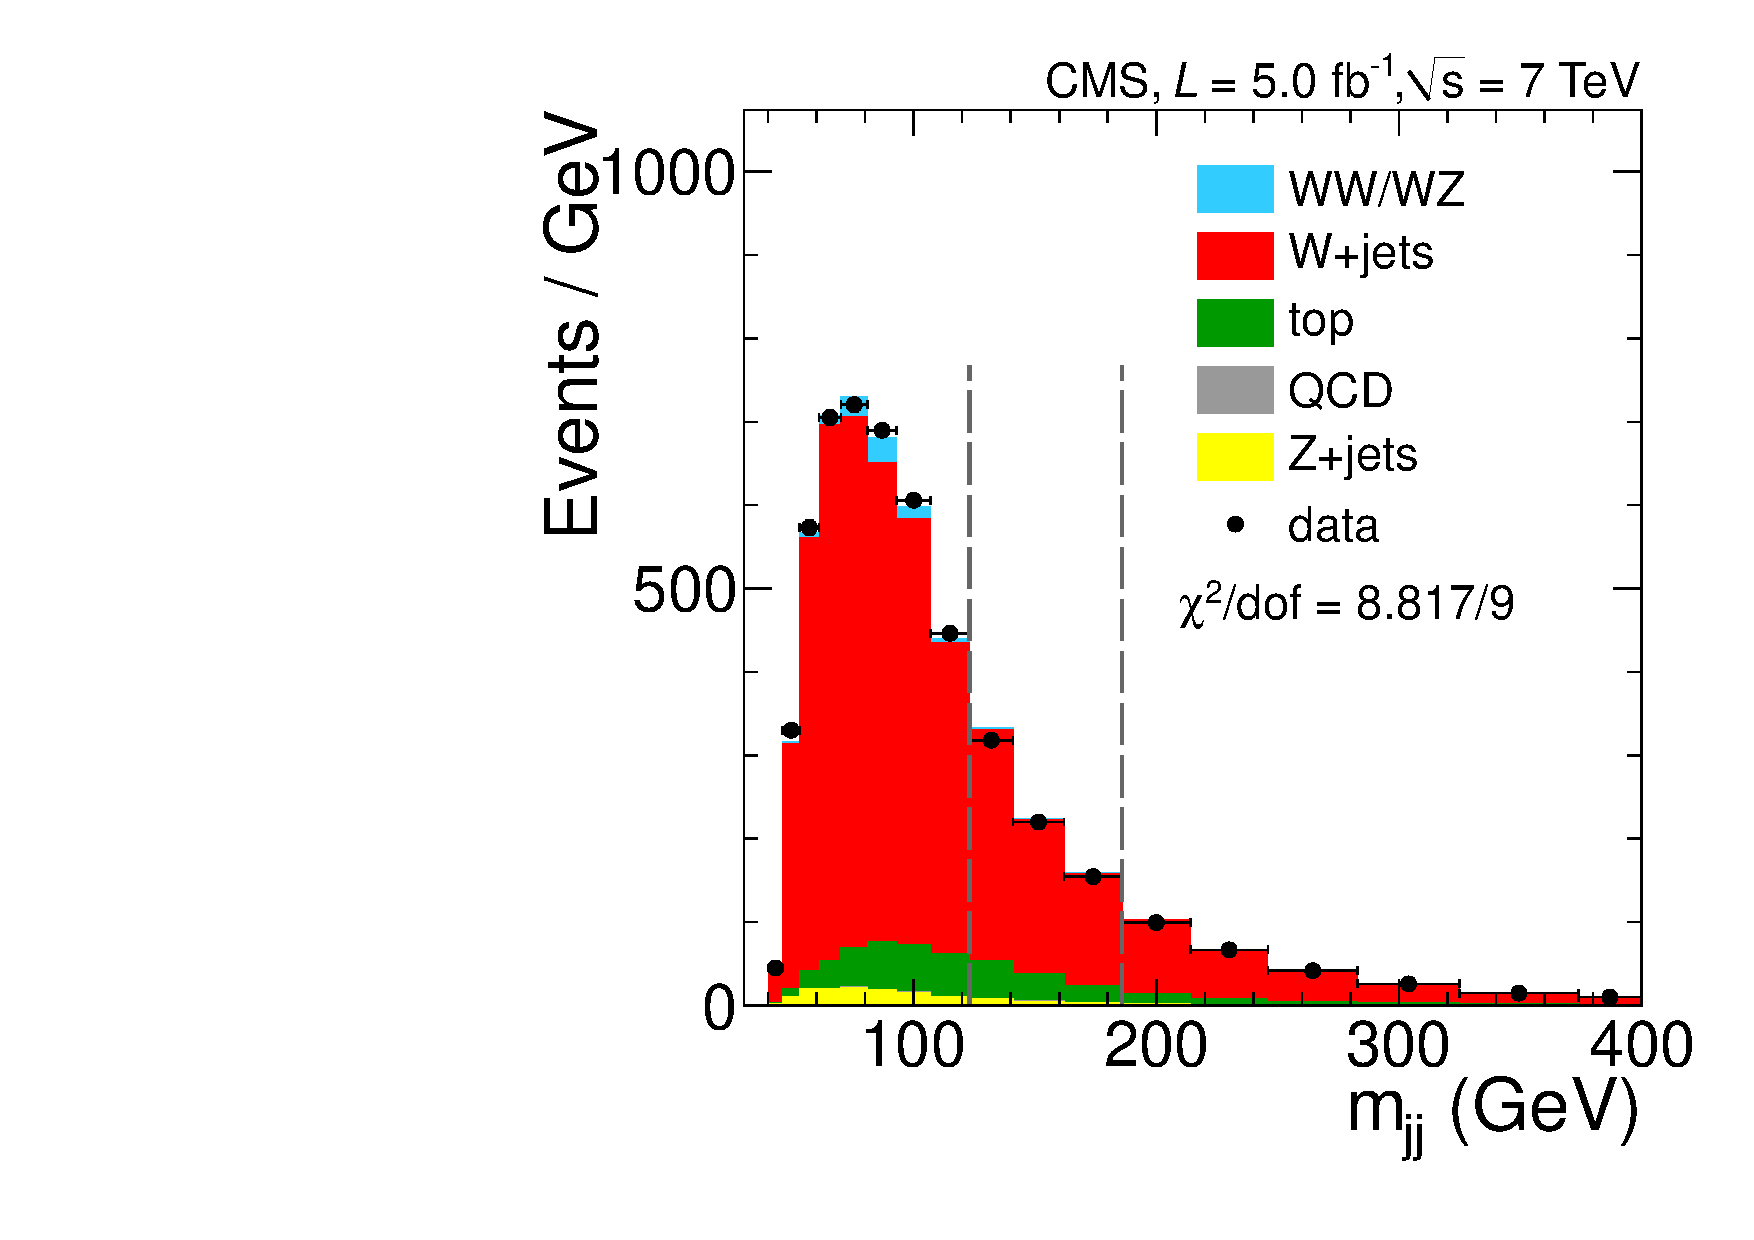
\includegraphics[trim = 2.5mm 1.5mm 2mm 1mm, clip, width=0.255\textwidth]{figs/Wjj_Mjj_Muon_2jets_Stacked.pdf}
%  }   
%  \subfigure[]{
%  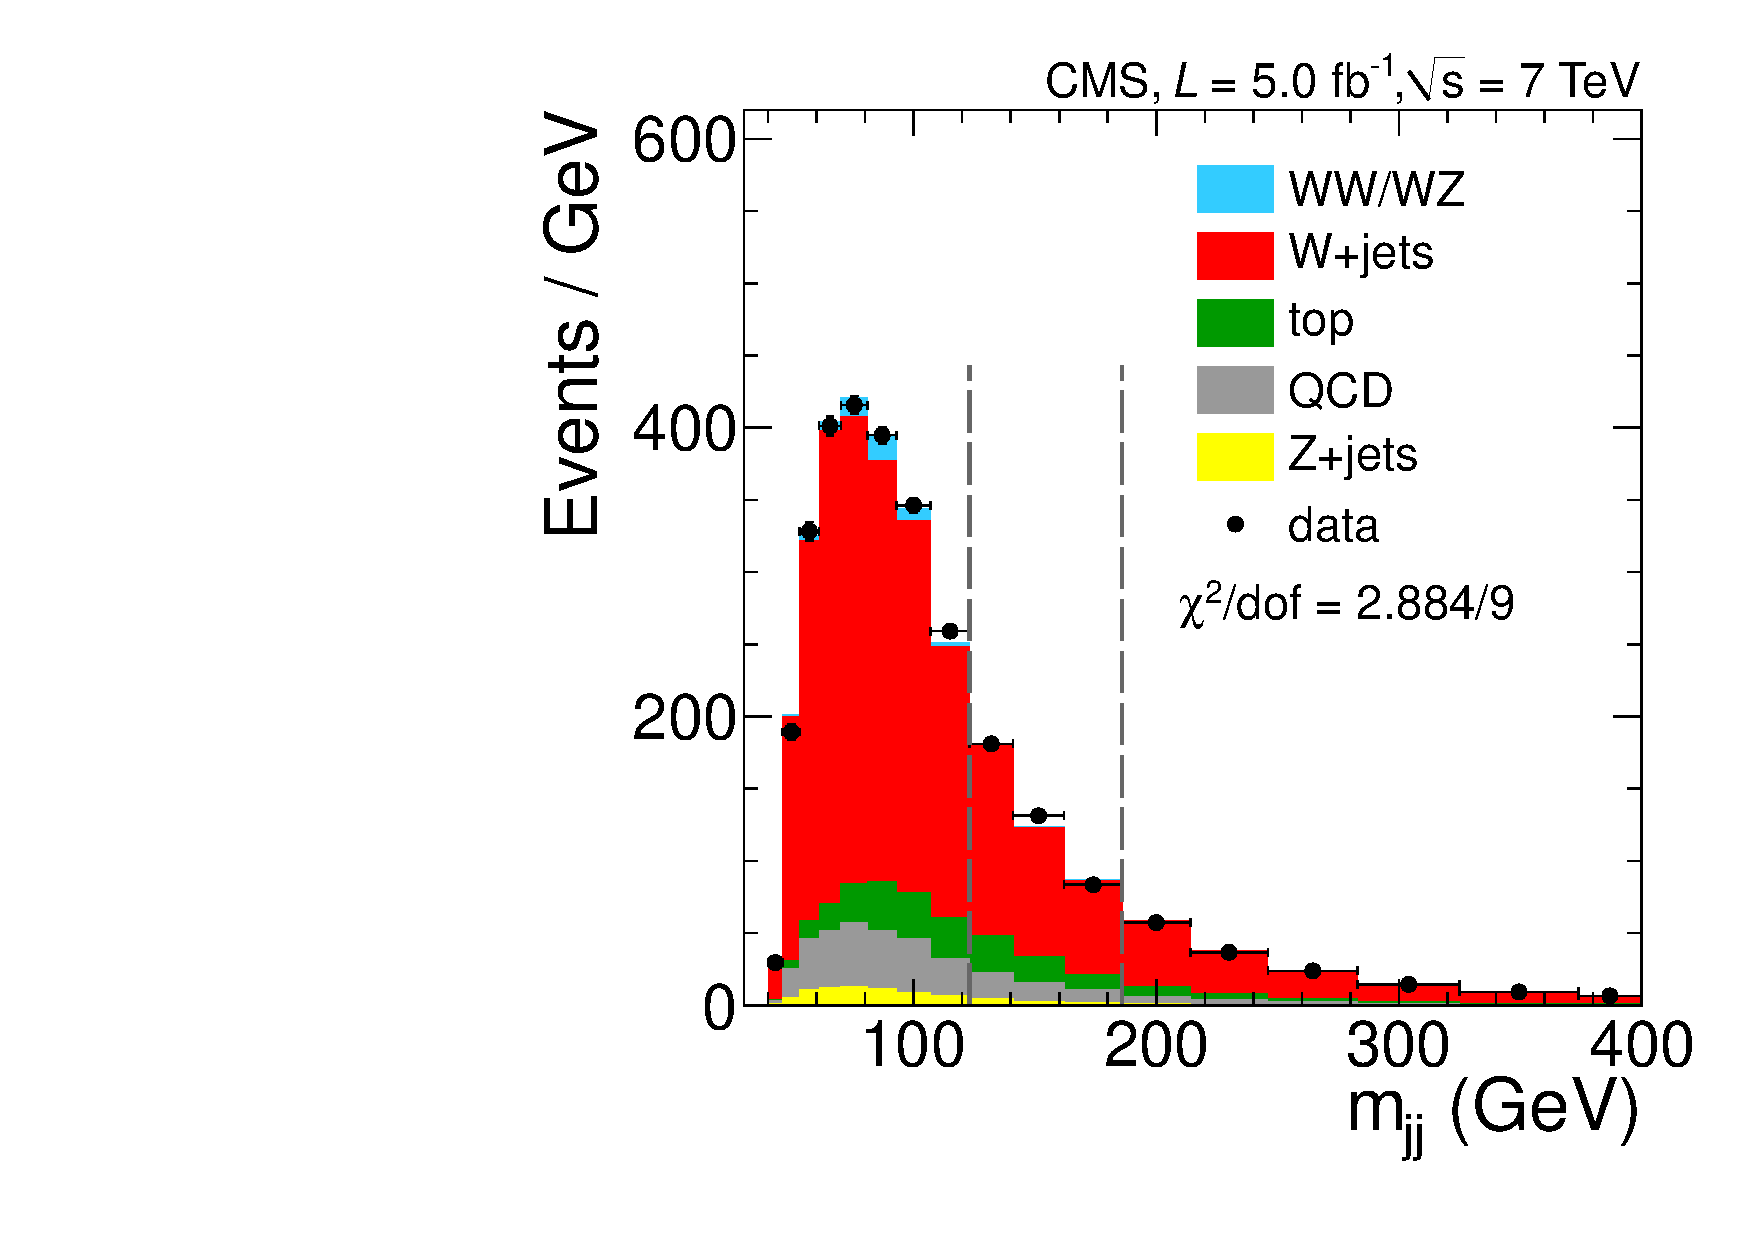
\includegraphics[trim = 16mm 1.5mm 2mm 1mm, clip, width=0.238\textwidth]{figs/Wjj_Mjj_Electron_2jets_Stacked.pdf}
%  }   
%   \subfigure[]{
%   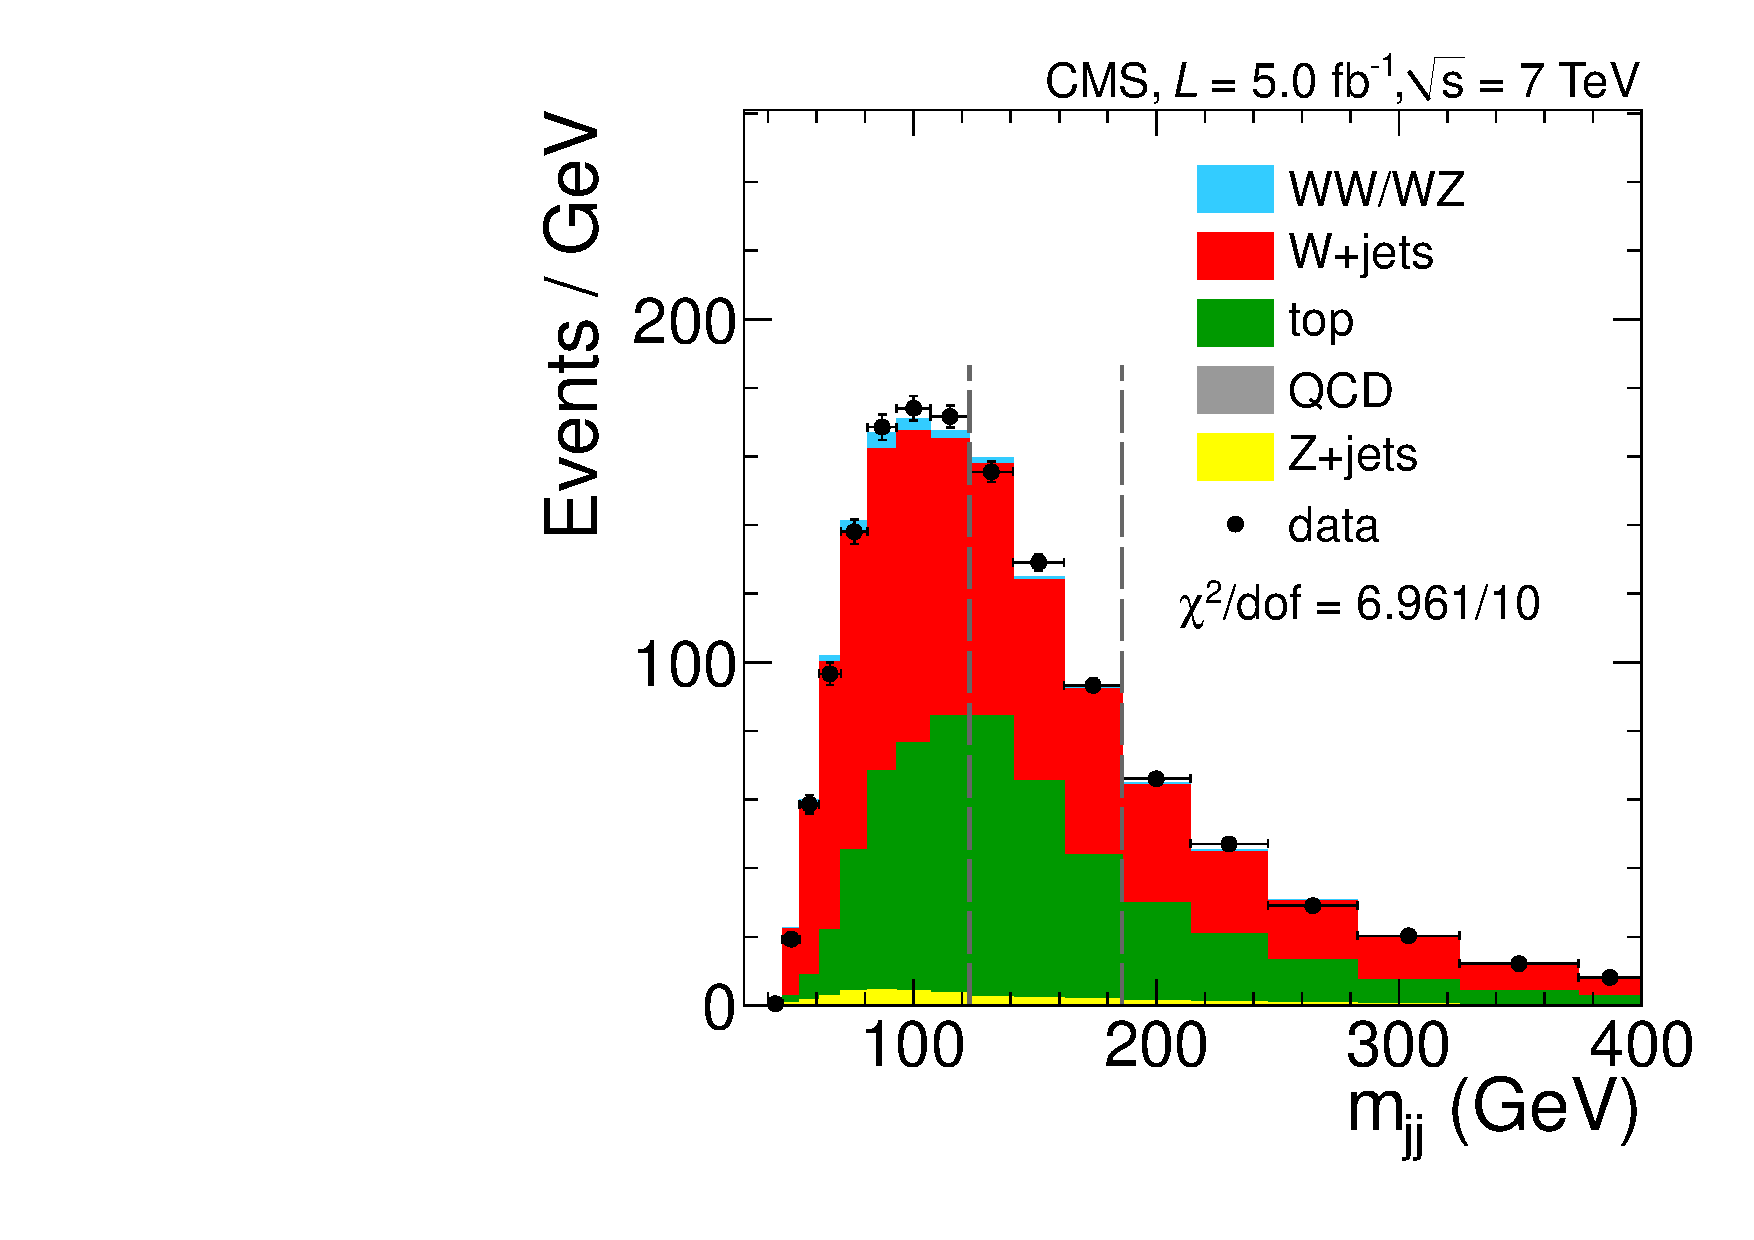
\includegraphics[trim = 16mm 1.5mm 2mm 1mm, clip, width=0.238\textwidth]{figs/Wjj_Mjj_Muon_3jets_Stacked.pdf}
%   }
%   \subfigure[]{
%   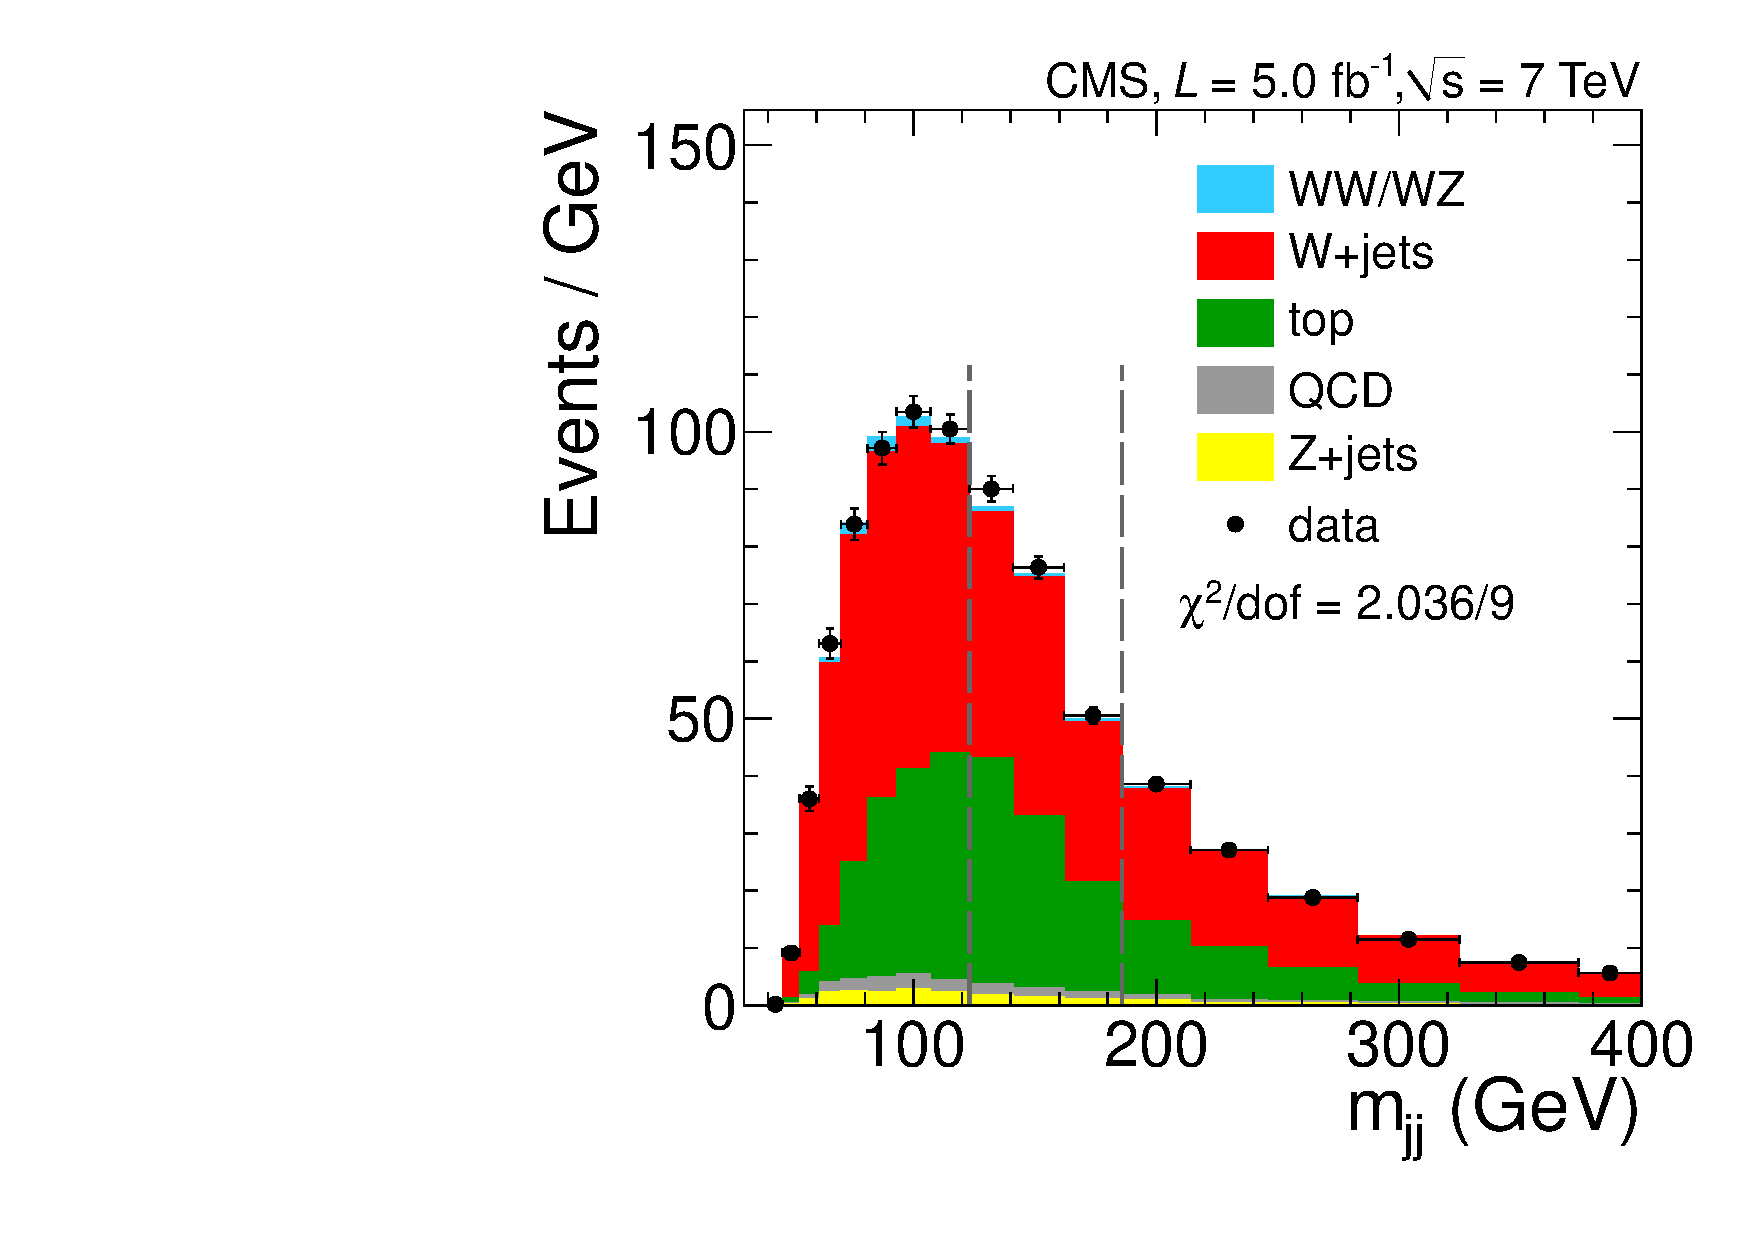
\includegraphics[trim = 16mm 1.5mm 2mm 1mm, clip, width=0.238\textwidth]{figs/Wjj_Mjj_Electron_3jets_Stacked.pdf}
%   }
%\vspace*{1mm} \\
%  \subfigure[]{
%  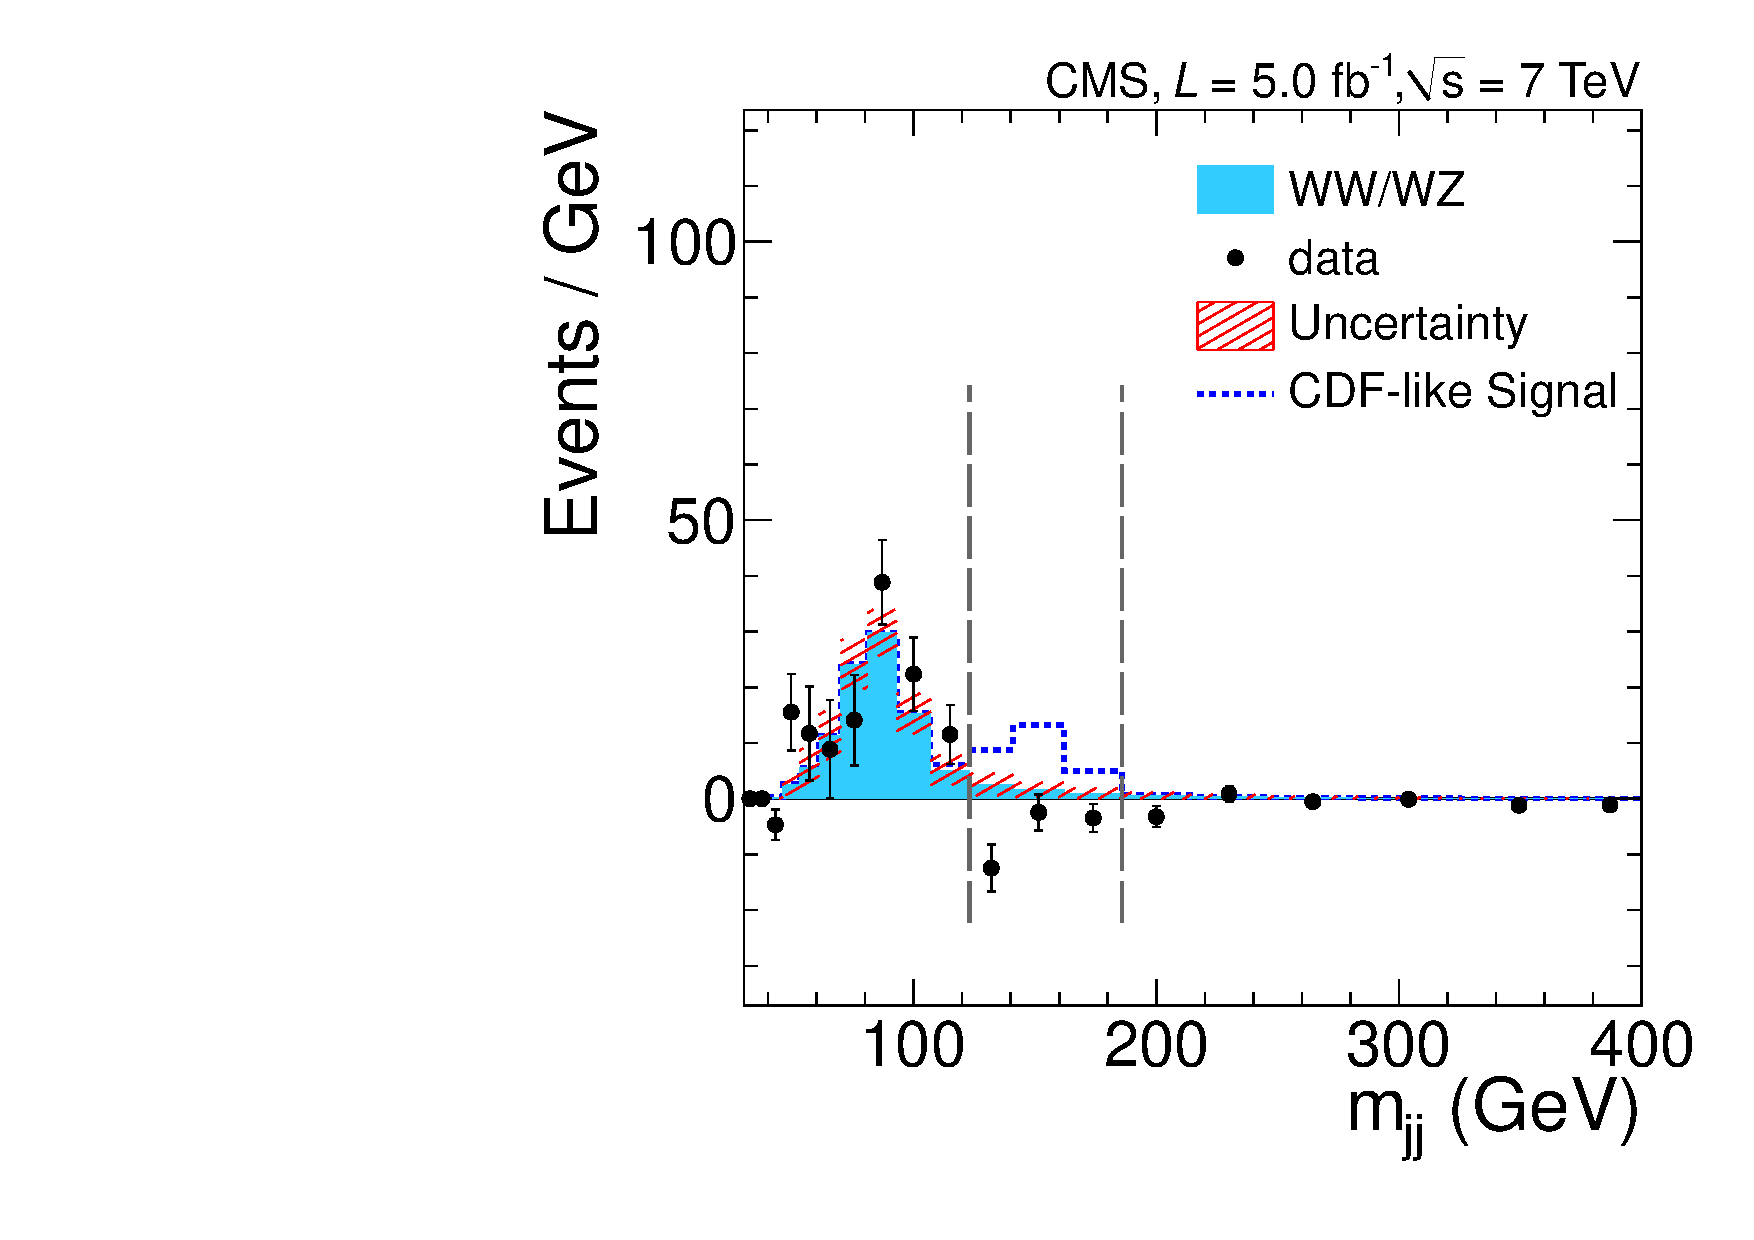
\includegraphics[trim = 2.5mm 1.5mm 2mm 1mm, clip, width=0.255\textwidth]{figs/Wjj_Mjj_Muon_2jets_Subtracted.pdf}
%   }
%  \subfigure[]{
%  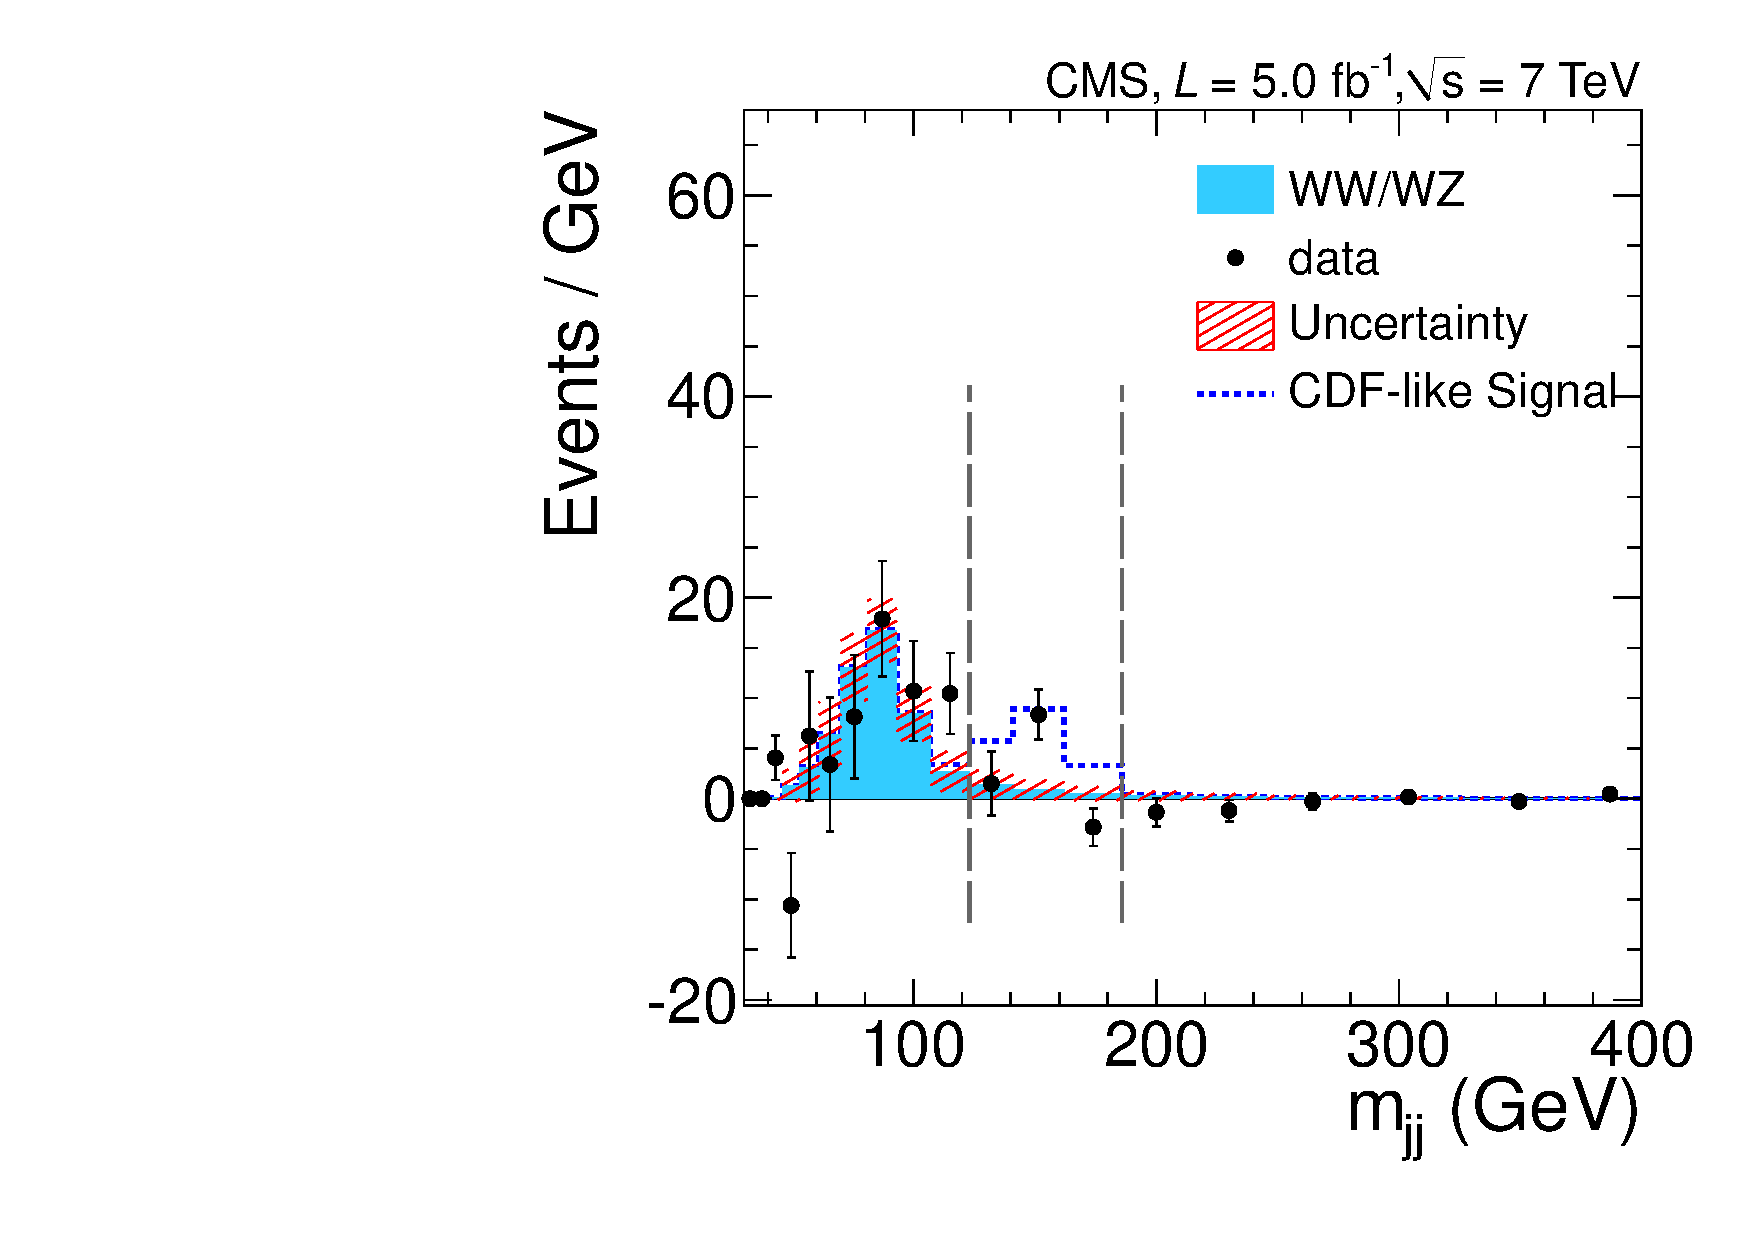
\includegraphics[trim = 16mm 1.5mm 2mm 1mm, clip, width=0.238\textwidth]{figs/Wjj_Mjj_Electron_2jets_Subtracted.pdf}
%   }
%   \subfigure[]{
%   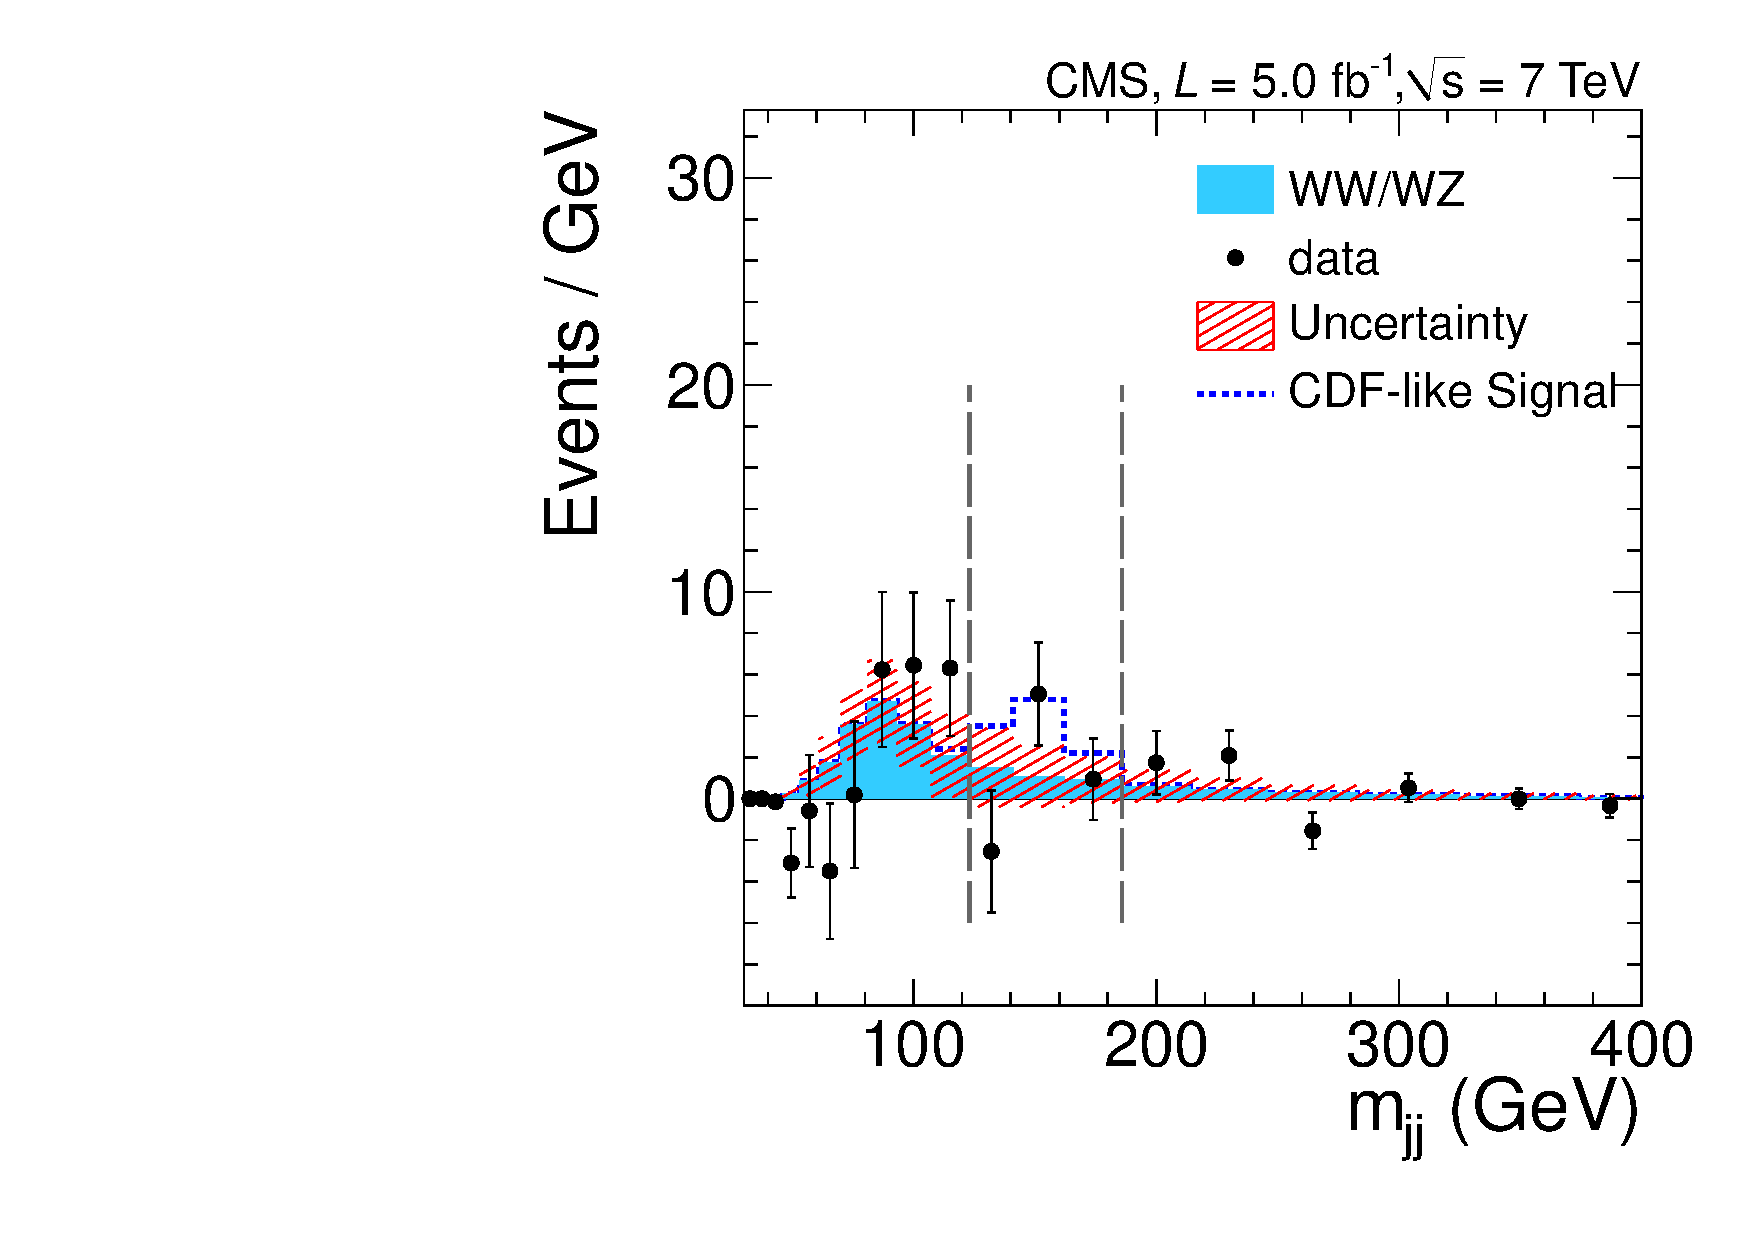
\includegraphics[trim = 16mm 1.5mm 2mm 1mm, clip, width=0.238\textwidth]{figs/Wjj_Mjj_Muon_3jets_Subtracted.pdf}
%   }
%   \subfigure[]{
%   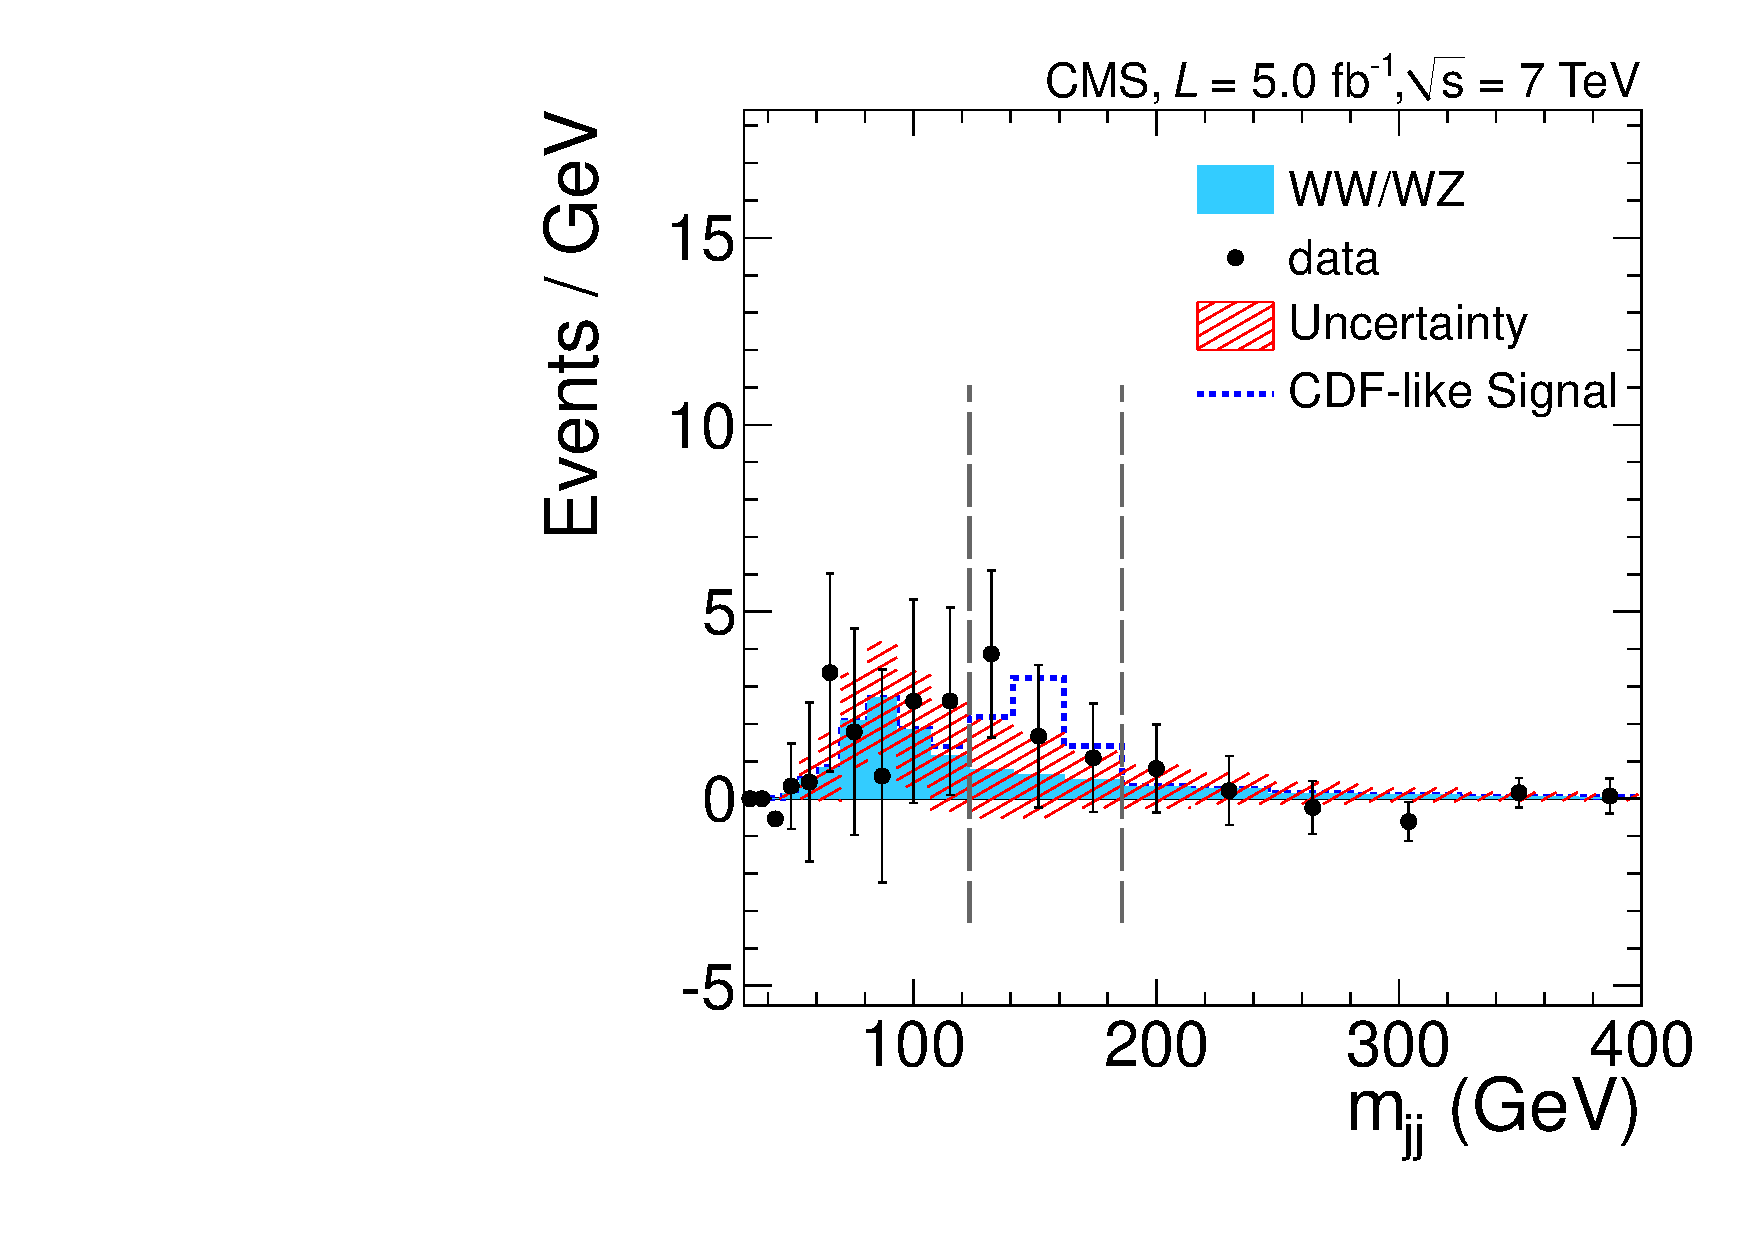
\includegraphics[trim = 16mm 1.5mm 2mm 1mm, clip, width=0.238\textwidth]{figs/Wjj_Mjj_Electron_3jets_Subtracted.pdf}
%   }
%   \caption{Upper row: Distribution of the invariant mass spectrum of the leading two jets observed 
%in data for different data categories: (a) muon plus 2 jets, (b) electron plus 2 jets, 
%(c) muon plus 3 jets, and 
%(d) electron plus 3 jets. Overlaid are the template distributions used in the likelihood
%fit to the measured \mjj distibution, with their relative normalization as obtained in the fit.
%In the fit the region between the vertical dotted lines is excluded.
%Lower row: The measured \mjj distribution after subtraction of all SM template distributions
%with the exception of the $WW/WZ$ one, shown in respective order (e--h)
%for the different data categories. Depicted is the number of events per GeV, i.e., the raw event count can be obtained by 
%multiplying with the bin width.
%Error bars correspond to the statistical errors only. The vertical dotted lines indicate the interval excluded from the fit.
%}
%\label{fig:Fig1}}
%\end{figure}
%%%%%%%%%%%%%%%%%%%%
%%%%%%%%%%%%%%%%%%%%                                                                         
\begin{figure}[h!]
  {\centering
  \subfigure[]{
    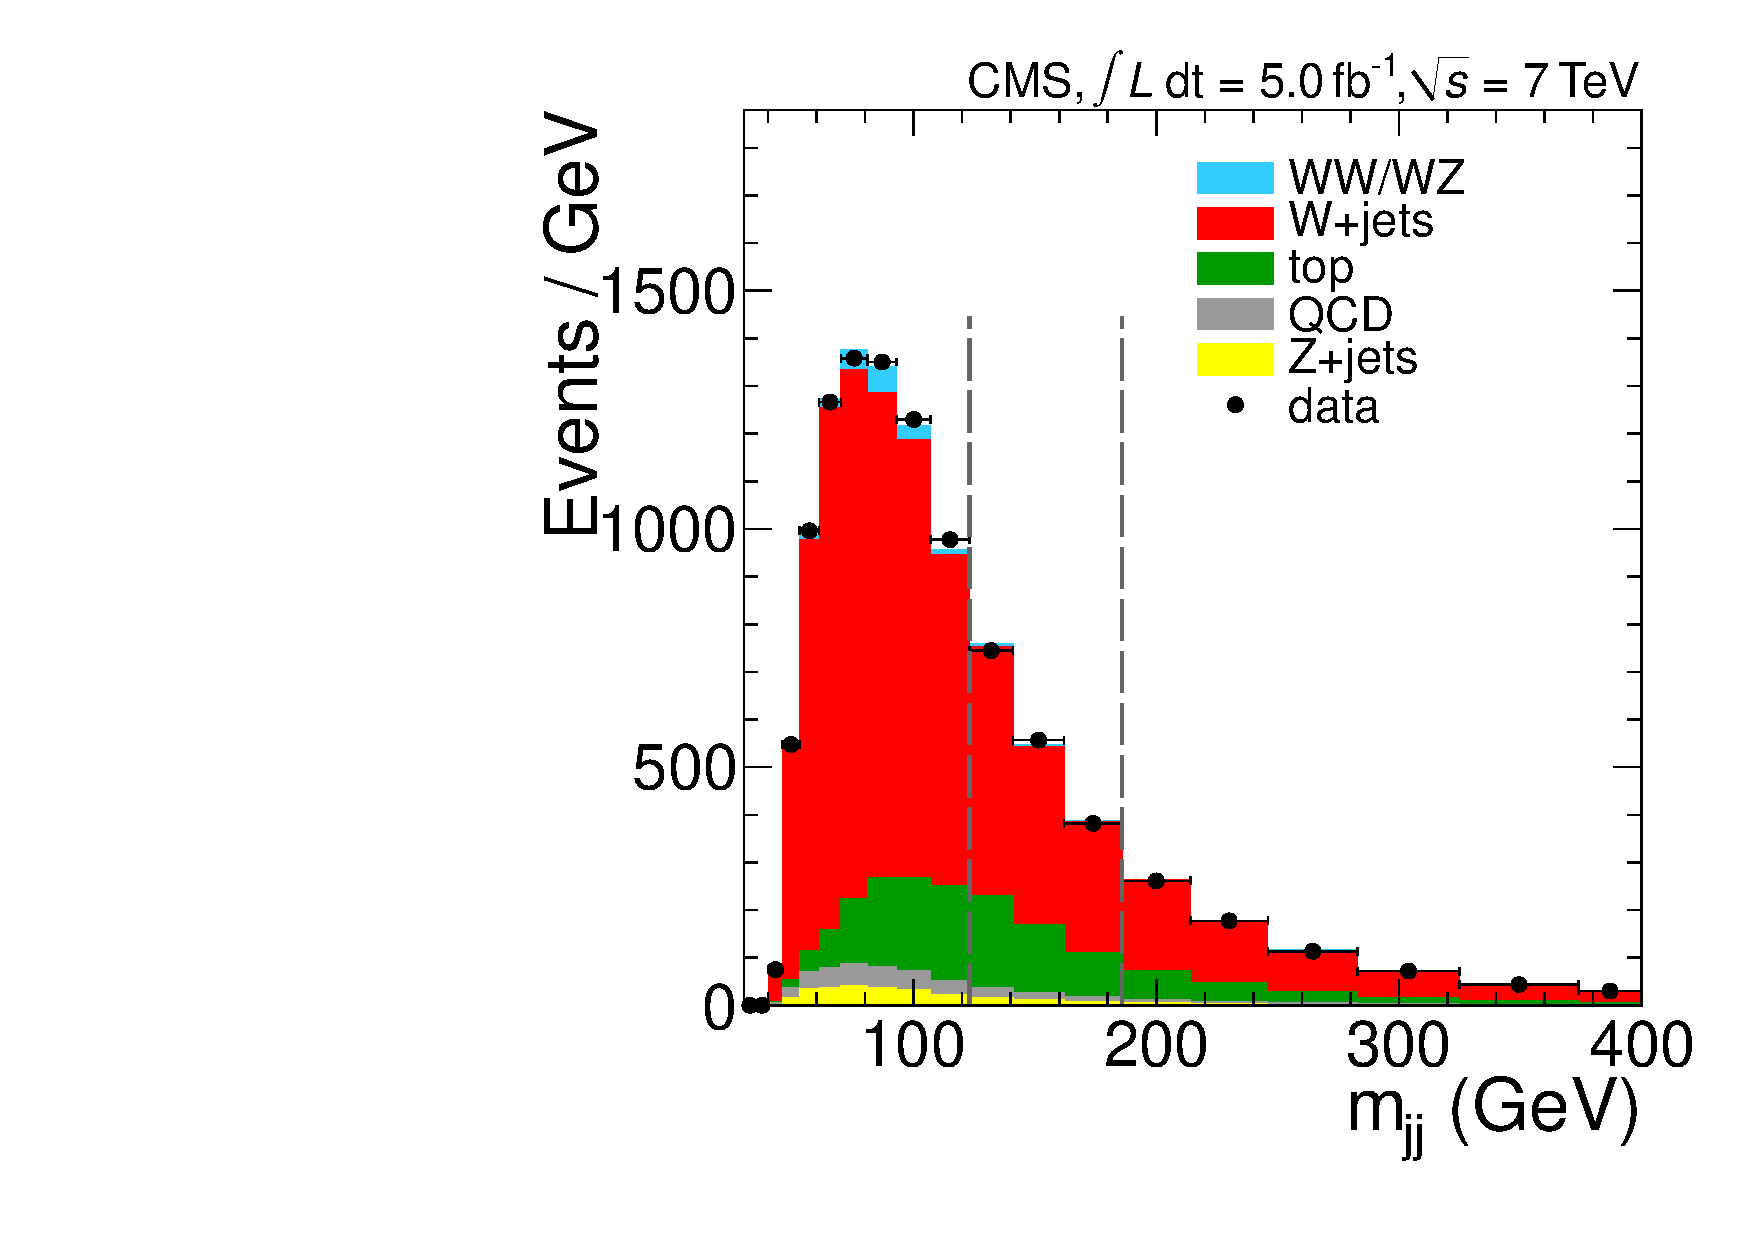
\includegraphics[width=0.32\textwidth]{figs/Mjj_Stacked_combined.pdf}
    }  
  \subfigure[]{ 
    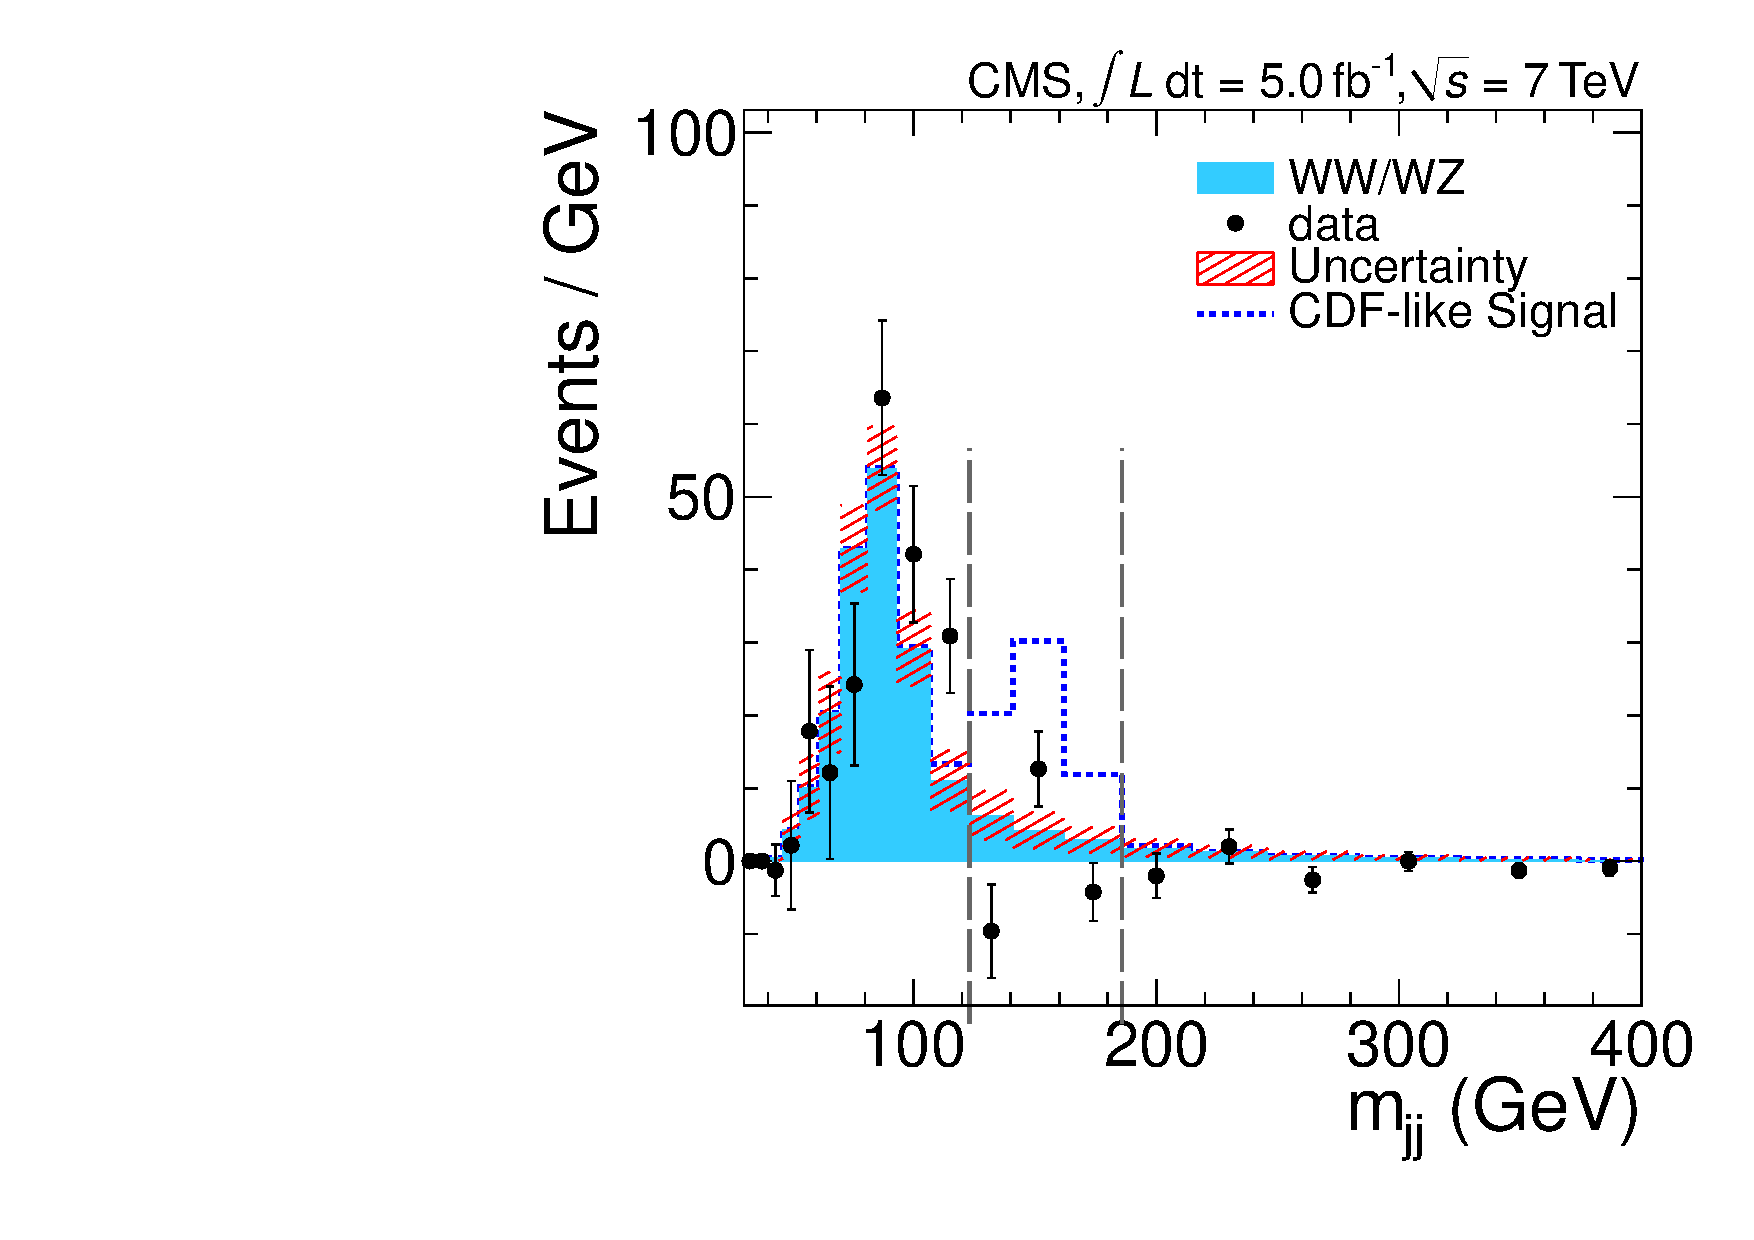
\includegraphics[width=0.32\textwidth]{figs/Mjj_Subtracted_combined.pdf}
    }
  \subfigure[]{
    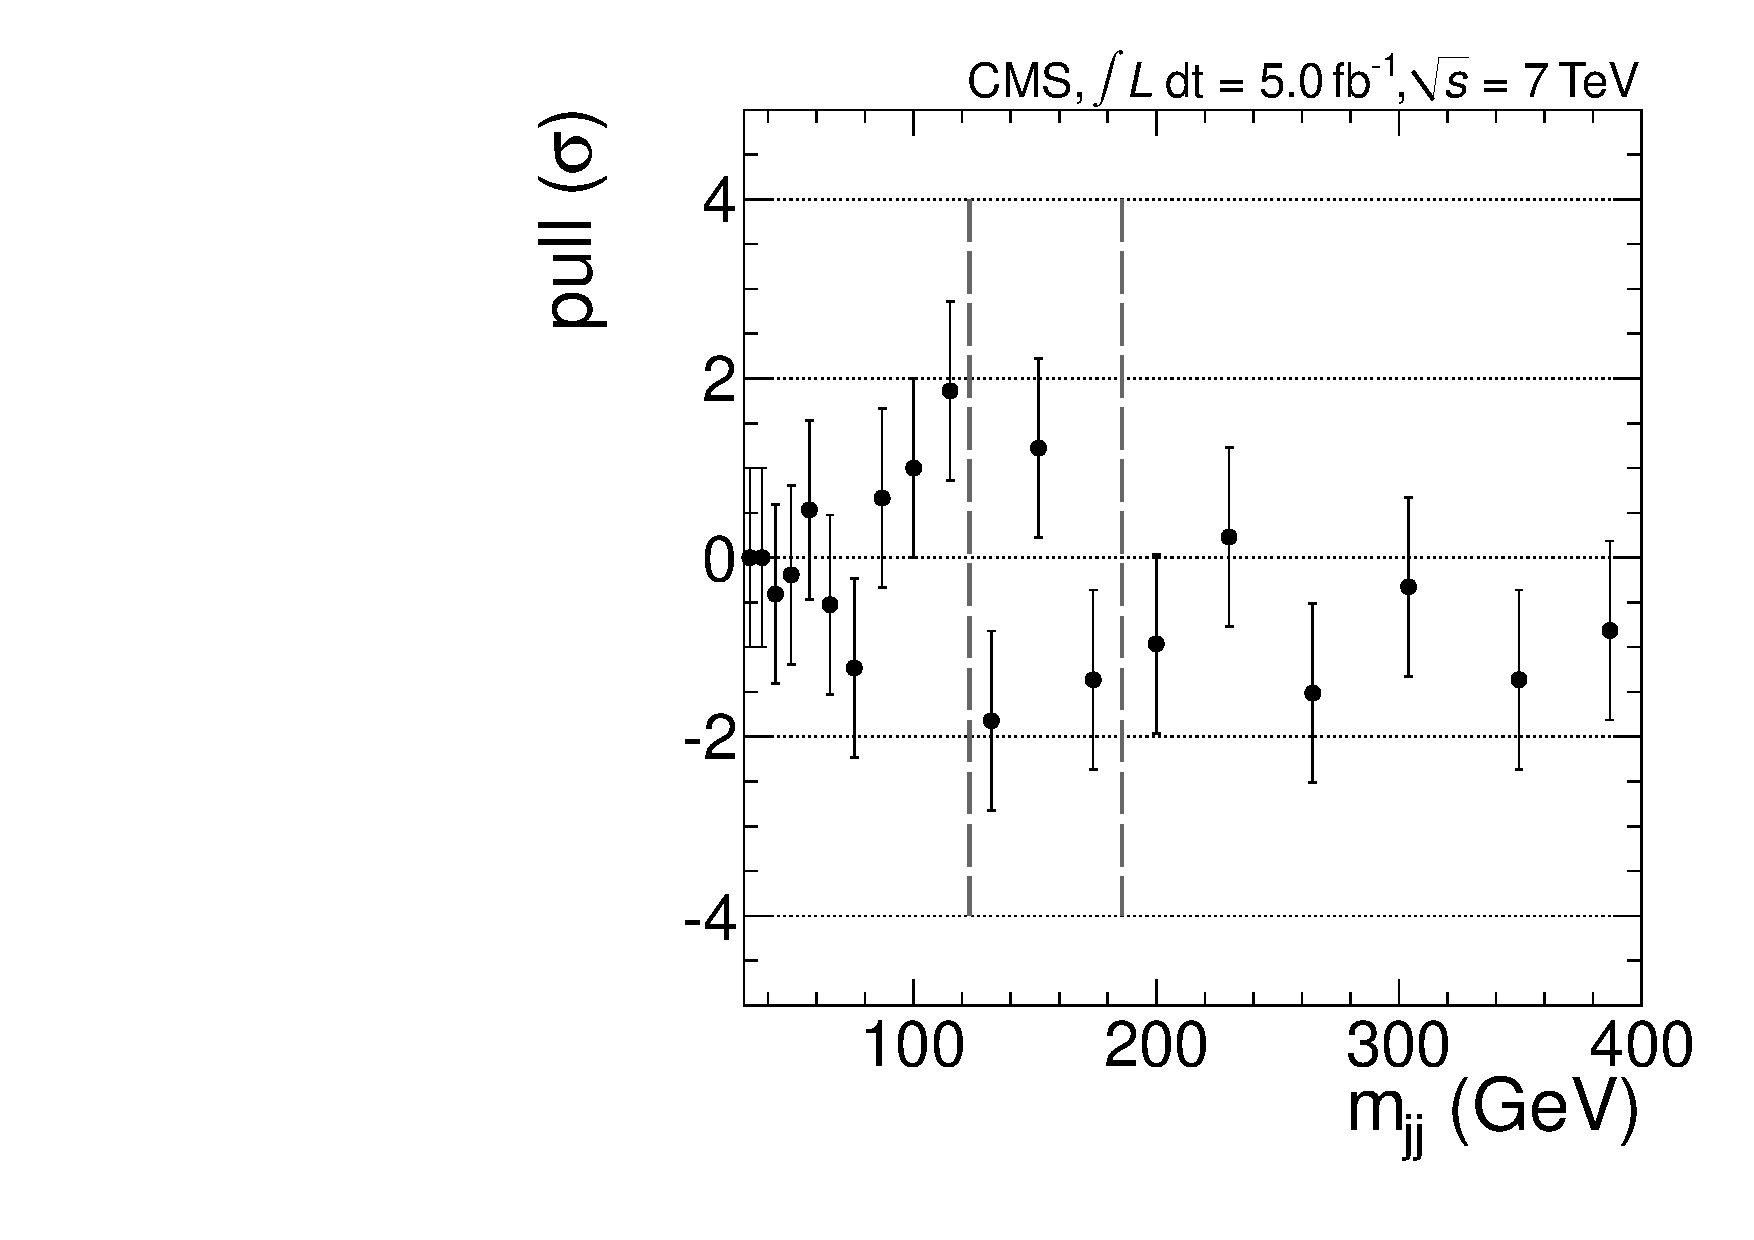
\includegraphics[width=0.32\textwidth]{figs/Mjj_Pull_combined.pdf}
    }
 \caption{(a) Distribution of the invariant mass spectrum of the 
 leading two jets observed in data including all four categories combined  
 (muon plus 2 jets, muon plus 3 jets, electron plus 2 jets, and      
 electron plus 3 jets). Overlaid are the template distributions used 
 in the likelihood fit to the measured \mjj distibution, with their 
 relative normalization as obtained from the fit.              
 The region between the vertical dotted lines is excluded in the fit.       
 Depicted is the number of events per GeV, \textit{i.e.}, the raw event count can be obtained by
 multiplying with the bin width.                              
 (b) The same distribution after subtraction of all SM components   
 except the electroweak diboson WW/WZ. 
 Error bars correspond to the statistical uncertainty. 
 The band represents the systematic uncertainty in the sum of the SM components. 
 (c) The normalized residual: [data - fit] / fit uncertainty.}
    \label{fig:Fig1}}
\end{figure}
%%%%%%%%%%%%%%%%%%%%



%%%%%%%%%%%%%%%
\begin{table}[!htbp]
   \begin{center}
  \caption{Event yields determined from a likelihood fit to the data. 
  The total uncertainty includes the effect of correlation among the 
  individual contributions using the full covariance matrix.}
  \label{tab:yields}
  \begin{tabular} {l  c  c c c }
    \hline \hline
    Process             &    \multicolumn{2}{c}{Muon channel} & \multicolumn{2}{c}{Electron channel} \\
\hline
                        &    2 jets         &  3 jets         & 2 jets           &  3 jets\\
\hline
    W plus jets         &    58919$\pm$530  &  13069$\pm$366  &  29787$\pm$1153  &  8397$\pm$292\\
    Dibosons            &    1236$\pm$114   &  333$\pm$32     &  685$\pm$65      &  184$\pm$18\\
    \ttbar              &    4570$\pm$307   &  9049$\pm$382   &  2556$\pm$174    &  4265$\pm$253\\
    Single top          &    1765$\pm$87    &  1001$\pm$50    &  916$\pm$46      &  521$\pm$26\\
    Drell-Yan plus jets &    1837$\pm$79    &  561$\pm$24     &  1061$\pm$46     &  364$\pm$16\\
    Multijet            &    29$\pm$284     &  0 $\pm$ 90     &  3944$\pm$1133   &  324$\pm$160\\
\hline
   Fit $\chi^2$ probability&   0.454        & 0.729           &  0.969           & 0.991    \\
    Total from fit      &    68294$\pm$307  &  24013$\pm$193  &  38949$\pm$228   &  14055$\pm$143\\
    Data                &    67900          &  24046          &  38973           &  14145 \\
\hline
\multicolumn{5}{c}{In the test region $123\,\text{GeV} < m_{jj} <186\,\text{GeV}$} excluded from the fit\\
\hline
   Total                & 14511$\pm$125     & 7739$\pm$95     & 7944$\pm$92      &  4347$\pm$70\\
   Data                 & 14050             & 7751            & 8023             &  4438 \\
\hline \hline
  \end{tabular}
\end{center}
\end{table}
%%%%%%%%%%%%%%%%%%%%%%%%%%%%%%%%%%%%%%%%%%%%%%%%%%%%%%%%%%%%
%%%%%%%%%%%%%%%%%%%%%%%%%%%%%%%%%%%%%%%%%%%%%%%%%%%%%%%%%%%%

%%%%%%%%%%%%%%
Figure~\ref{fig:Fig1}a shows the observed \mjj 
distribution for all four channels combined, together with the contribution of various 
SM processes whose normalizations are obtained from the fit. 
Figure~\ref{fig:Fig1}b shows the same distribution after subtracting 
all SM contributions from data except for electroweak diboson 
WW/WZ events.
Except for a peak near 80 GeV from diboson events no 
other peak is visible in the entire spectrum.
Figure~\ref{fig:Fig1}c shows the normalized residual, 
\textit{i.e.}, pull distribution defined as  
[data - fit]/ fit uncertainty, where the uncertainty 
is the combined statistical and systematic one.
Table~\ref{tab:yields} presents the yields of various SM 
components obtained from the fit. 
The sum of all the contributions is compared with the number 
of observed data events. All numbers but those in the last two rows are for the
\mjj range [40, 400]~GeV. 
The last two rows compare the observed and fitted contributions 
in the \mjj range [123, 186]~GeV that is excluded in the fit.
The data agree with the SM expectation throughout, and we 
find no significant excess in the test region.  

\section{Fit validation and systematic error estimate}

We validate the fit procedure by  performing pseudo-experiments. 
In each experiment, we generate the \mjj distribution of the SM processes 
of the sample size observed in data, 
taking into account the correlation among the yields.  
We then repeat the fit on each sample. 
The resulting yields and pull distributions indicate that the bias on the total yield is below 0.2\% and that the
fit understimates the yield uncertainty slightly. These
effects are corrected for in the final result. 
Uncertainties in the jet energy scale (JES) are 
estimated in a sample of W bosons decaying hadronically in a highly 
pure sample of semileptonic \ttbar\ events. 
The mean and resolution of the reconstructed dijet (\textit{i.e.,} W) 
mass distribution in data agree within 0.6\% with the expectation from 
simulation, for the same level of the statistical accuracy as the measurement. 
This good agreement is further confirmed by including an additional free parameter in the fit to allow
for shifts of the JES between data and simulation.
A small difference in \MET resolution~\cite{Chatrchyan:2011tn} between
data and simulation affects  the signal acceptance for the new physics models
under consideration at the 0.5\% level.
Further systematic uncertainties are due to the uncertainty of the trigger efficiency 
estimates in data, which is 1\%, and the estimate of lepton reconstruction and selection 
efficiency, which is 2\%~\cite{WZCMS:2010}. 
The uncertainty in the luminosity determination is 2.2\%~\cite{lumiPAS}.
 
\section{Results on presence of possible resonant enhancement}

We investigate the presence of a possible resonant enhancement
in the dijet mass spectrum near $150~\gev$ for the technicolor, 
the leptophobic $\Zo^\prime$, the WH, and a generic Gaussian signal model obtained
from a delta function at $\mjj=150$~GeV convolved with the CMS detector resolution of 15~GeV. 
The number of expected signal events $N^{Signal}$ at the LHC for a given 
cross section at the Tevatron 
can be determined by considering the ratio of the predicted cross sections 
for our reference process, that is, $WH$ production with $M_H = 150$~GeV. 
This process is dominated by quark-antiquark ($q\overline{q}$) annihilation.  
Since $q\overline{q}$ processes have the smallest increase in partonic luminosity 
from Tevatron to LHC, this choice provides a conservative limit. 
%%\begin{equation}
%%%\sigma_{\textrm{LHC}}^{dijet-resonance}  \times BR(W\to\ell\nu)=  
%%N_{\textrm LHC}^{dijet-resonance} = 
%%\sigma_{\textrm{Tevatron}}^{dijet-resonance}  \times BR(W\to\ell\nu) \times \frac{\sigma_{\textrm{LHC}}^{WH}}{\sigma_{\textrm{Tevatron}}^{WH}} \times (\varepsilon\times\cal{A}) \times \int \cal{L} \textrm{dt},  
%%\label{eqTevToLHC}
%%\end{equation}
%%
\begin{eqnarray}
\sigma_{\textrm{LHC}}^{dijet-resonance} &=& 
\sigma_{\textrm{Tevatron}}^{dijet-resonance}  \times \frac{\sigma_{\textrm{LHC}}^{WH}}{\sigma_{\textrm{Tevatron}}^{WH}},\label{eqTevToLHC2}\\
N^{Signal} &=&   \sigma_{\textrm{LHC}}^{dijet-resonance} \times BR(W\to\ell\nu) \times (\varepsilon\times\cal{A}) \times \int \cal{L} \textrm{dt}, 
\label{eqTevToLHC}
\end{eqnarray}
%%%%%%%%%%%%%%
where $\sigma_{\textrm{LHC}}^{WH} = 46.8~\textrm{fb}$~\cite{LHC4PDFxsec} and 
$\sigma_{\textrm{Tevatron}}^{WH} = 12~\textrm{fb}$~\cite{Djouadi199856} are the 
theory cross sections for WH production at the LHC and the Tevatron, respectively, 
$\varepsilon\times\cal{A}$ denotes $\textrm{efficiency} \times \textrm{acceptance}$ for WH events, 
$BR$ stands for branching fraction~\cite{pdg}, 
and $\int \cal{L} \textrm{dt}$ is the integrated luminosity.
The values of cross section and $\varepsilon\times\cal{A}$ for 
these models are given in Table~\ref{tab:signals}.
A generic Gaussian signal normalized to  
$\sigma_{\textrm{Tevatron}} = \textrm{4~pb}$ corresponds 
to $\sigma_{\textrm{LHC}}\times BR(W\to\ell\nu) = \textrm{3.4~pb}$.
%%%%%%%%%%%%%%%%%%%%%%%%%%%%%
\begin{table}[bthp]
\begin{center}
  \begin{tabular}{l c c c c c}
    \hline  \hline
    Signal Model &  $\sigma \times BR$ (pb) & \multicolumn{4}{c}{$\varepsilon\times\cal{A}$} \\\hline
    &  & electron 2 jets & electron 3 jets & muon 2 jets & muon 3 jets \\
    \hline
    WH                & 0.0145 &  0.038 & 0.013 & 0.060 & 0.019 \\
    Technicolor ~\cite{Eichten:2011sh,AMartinMC}      & 1.58   &  0.039 & 0.011 & 0.065 & 0.020 \\
    $\Zo^{\prime}$~\cite{Buckley:2011vc,BuckleyMC}    & 1.72   &  0.042 & 0.014 & 0.070 & 0.023 \\
    \hline  \hline
  \end{tabular}
\end{center}
\caption{\label{tab:signals}
The cross section times W$\to\ell\nu$ branching ratio for 
various signal models and their overall reconstruction efficiency.}
\end{table}
%%%%%%%%%%%%%%%%%%%%%%%%%%%%%
%%%%%%%%%%%%%%%%%%%
\begin{figure}[bthp!]
\subfigure[]{
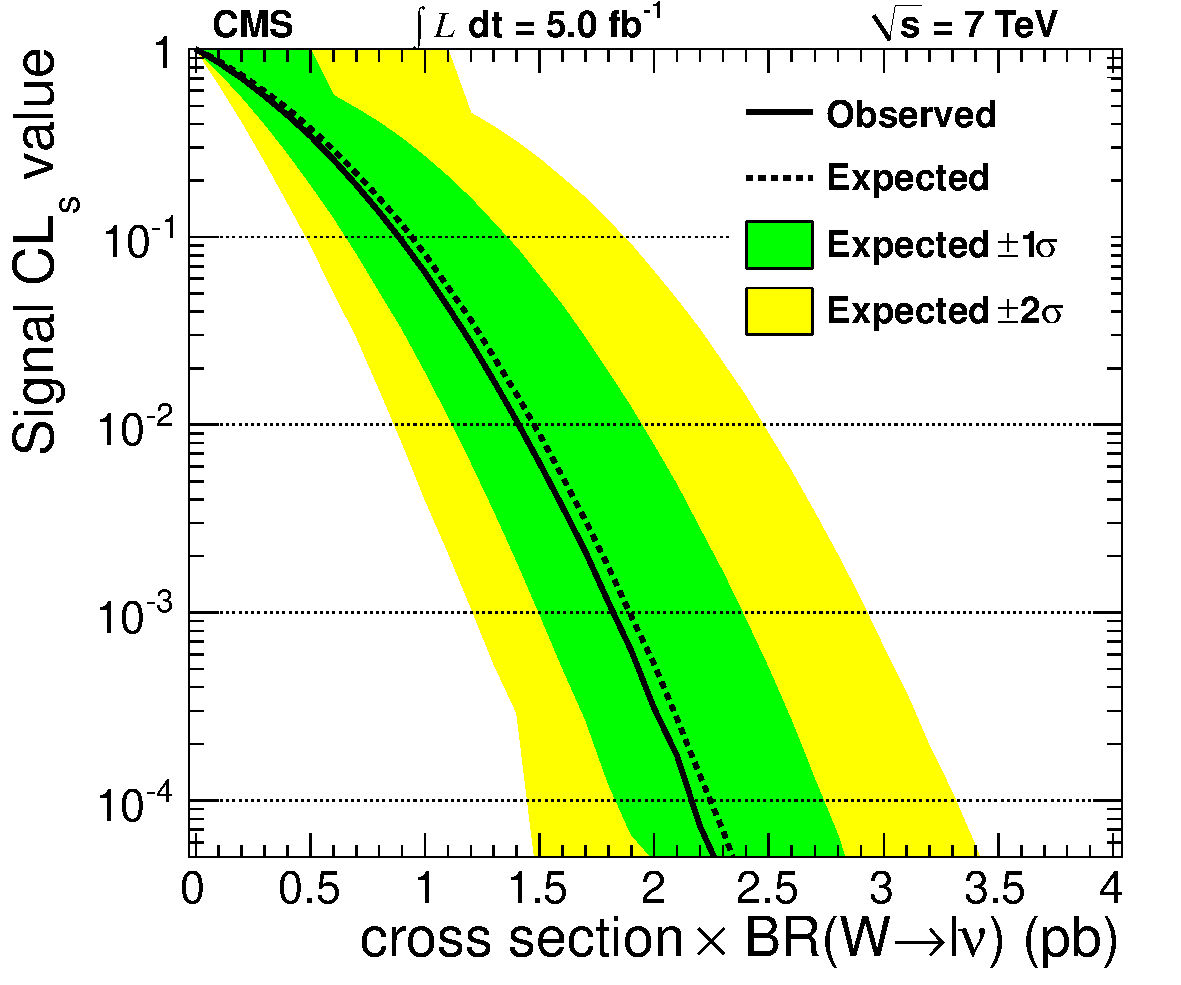
\includegraphics[trim = 0mm 1mm 0mm 0mm, clip, width=0.48\textwidth]{figs/mjjpvalues.pdf}
}
\hspace*{3mm} 
\subfigure[]{
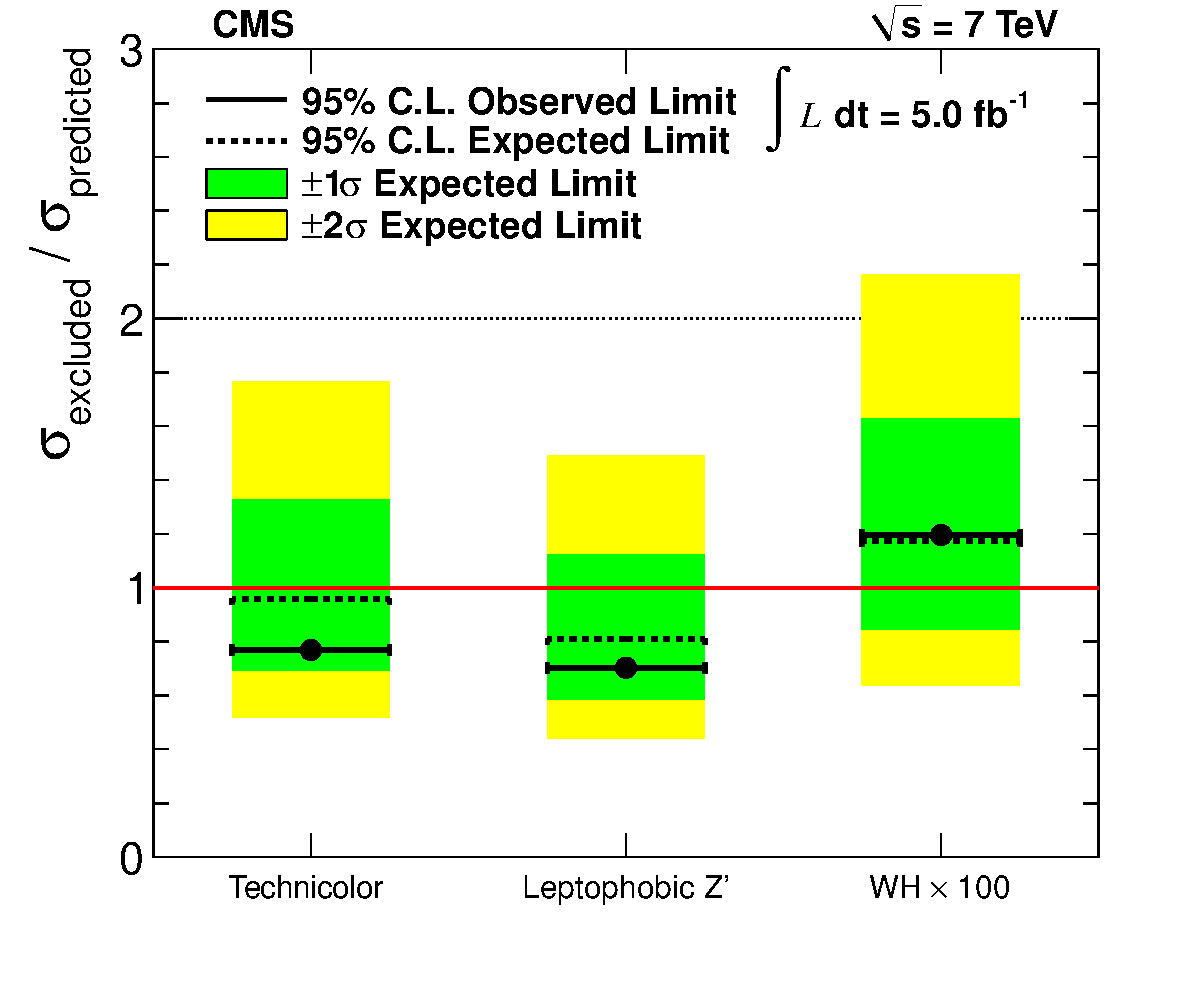
\includegraphics[trim = 0mm 1mm 0mm 0mm, clip, width=0.48\textwidth]{figs/mjjlimitbars.pdf}
}
\caption{\label{fig:Fig2} 
(a) The observed and expected values of the CL${}_{\textrm{S}}$ statistic for a
generic Gaussian signal hypothesis with M=150 GeV, width=15 GeV, as a
function of the cross section of the signal times the W$\to\ell\nu$ branching
fraction.
(b) Observed and expected 95\% CL upper limits, with one and two sigma
error bands, on the cross section for various signal models. The
limits were calculated using the CL${}_{\textrm{S}}$ method. A ratio of the excluded
cross section over the predicted cross section smaller than one
indicates that the model is excluded at 95\% CL.
Table~\ref{tab:signals} lists the cross sections for these models.
%The p-values for the same models are also shown in (a) as vertical lines. 
}
\end{figure}
%%%%%%%%%%%%%%%%%%%

Since we observe no resonant enhancement, we proceed to set    
exclusion limits using a modified frequentist 
CL${}_{\textrm{S}}$~\cite{pdg,CLS} with profile likelihood as the 
test statistic. 
Inputs to the limit setting procedure are the \mjj distribution 
obtained by combining the SM components from the fit, 
the observed distribution in data, and the expectation from 
the dijet resonance model under consideration.

Figure~\ref{fig:Fig2}a shows the distributions of 
observed and expected CL${}_{\textrm{S}}$ values 
for a generic Gaussian signal after combining the results of 
all four event categories.
We set an upper limit of 1.1~pb at 95\% confidence level (CL) 
on the production cross 
section $\times BR(W\to\ell\nu)$. 
%%which corresponds to a cross 
%%section of 1.5~pb at the Tevatron (Eq.~\ref{eqTevToLHC2}).
Upper limits on cross section computed at 95\% CL 
for the technicolor, the 
leptophobic $\Zo^\prime$, and the WH ($M_H = 150$~GeV) signal models are 
shown in Fig.~\ref{fig:Fig2}b.
%Their cross sections $\times BR(W\to\ell\nu)$ are 
%1.58 pb, 1.72 pb, and 0.0145 pb, respectively.
%An excess of the type reported by CDF, which corresponds to 
%$\sigma_{\textrm{LHC}}^{dijet-resonance}  \times BR(W\to\ell\nu) =  3.4$~pb, indicated as a vertical line 
%in Fig.~\ref{fig:Fig2}a, is excluded and we set an upper limit of 1.1~pb at 95\% CL on the production cross section 
%$\times BR(W\to\ell\nu)$ for such a resonance. 
The technicolor and $\Zo^\prime$ models are excluded.
%% at 90\% CL or higher.

\section{Summary}

%%%%%%%%%%%%%%%%%%%%%%
In summary, we have studied the invariant mass spectrum \mjj of the two jets with the highest transverse 
momenta 
in events with two or three jets produced in association with a W boson that decays leptonically.
The analyzed data sample corresponds to an integrated 
luminosity of 5.0~fb${}^{-1}$ collected with the CMS detector at 
$\sqrt{s} = 7$ TeV in 2010 and 2011. 
We find no evidence for a resonant enhancement near a dijet mass of 150~GeV.
Several 
theoretical models that predict the presence of a resonant 
enhancement near 150~GeV are excluded. 
%%%%%%%%%%%%%%%%%%%%%%%%%%%%%%%%%%%%%%%%%%%%%%%%%%%%%%%%%%%%%%%%%%%%%%%%%%




% >> acknowledgements (for journal papers)
% Please include the latest version from https://twiki.cern.ch/twiki/bin/viewauth/CMS/Internal/PubAcknow.
%\section*{Acknowledgements}
%We wish to congratulate our colleagues in the CERN accelerator departments for the excellent
%performance of the LHC machine. We thank the technical and administrative staff at CERN and other CMS
%institutes, and acknowledge support from: FMSR (Austria); FNRS and FWO (Belgium); CNPq, CAPES, FAPERJ,
%and FAPESP (Brazil); MES (Bulgaria); CERN; CAS, MoST, and NSFC (China); COLCIENCIAS (Colombia); MSES
%(Croatia); RPF (Cyprus); Academy of Sciences and NICPB (Estonia); Academy of Finland, MEC, and HIP
%(Finland); CEA and CNRS/ IN2P3 (France); BMBF, DFG, and HGF (Germany); GSRT (Greece); OTKA and NKTH
%(Hungary); DAE and DST (India); IPM (Iran); SFI (Ireland); INFN (Italy); NRF and WCU (Korea); LAS
%(Lithuania); CINVESTAV, CONACYT, SEP, and UASLP-FAI (Mexico); MSI (New Zealand); PAEC (Pakistan);
%MSHE and NSC (Poland); FCT (Portugal); JINR (Armenia, Belarus, Georgia, Ukraine, Uzbekistan); MON,
%RosAtom, RAS and RFBR (Russia); MSTD (Serbia); MICINN and CPAN (Spain); Swiss Funding Agencies
%(Switzerland); NSC (Taipei); TUBITAK and TAEK (Turkey); STFC (United Kingdom); DOE and NSF (USA).
%Individuals have received support from the Marie-Curie programme and the European Research Council
%(European Union); the Leventis Foundation; the A. P. Sloan Foundation; the Alexander von Humboldt
%Foundation; the Belgian Federal Science Policy Office; the Fonds pour la Formation \`a la Recherche
%dans l'\'industrie et dans l'\'Agriculture (FRIA-Belgium); the Agentschap voor Innovatie door Wetenschap
%en Technologie (IWT-Belgium); the Council of Science and Industrial Research, India; and the HOMING
%PLUS programme of Foundation for Polish Science, cofinanced from European Union, Regional Development
%Fund.
% ack-text

%% **DO NOT REMOVE BIBLIOGRAPHY**
%\newpage
\bibliography{auto_generated}   % will be created by the tdr script.

%% examples of appendices. **DO NOT PUT \end{document} at the end
\clearpage
\appendix
\section{Additional plots}


\begin{figure}[h!]
  {\centering
    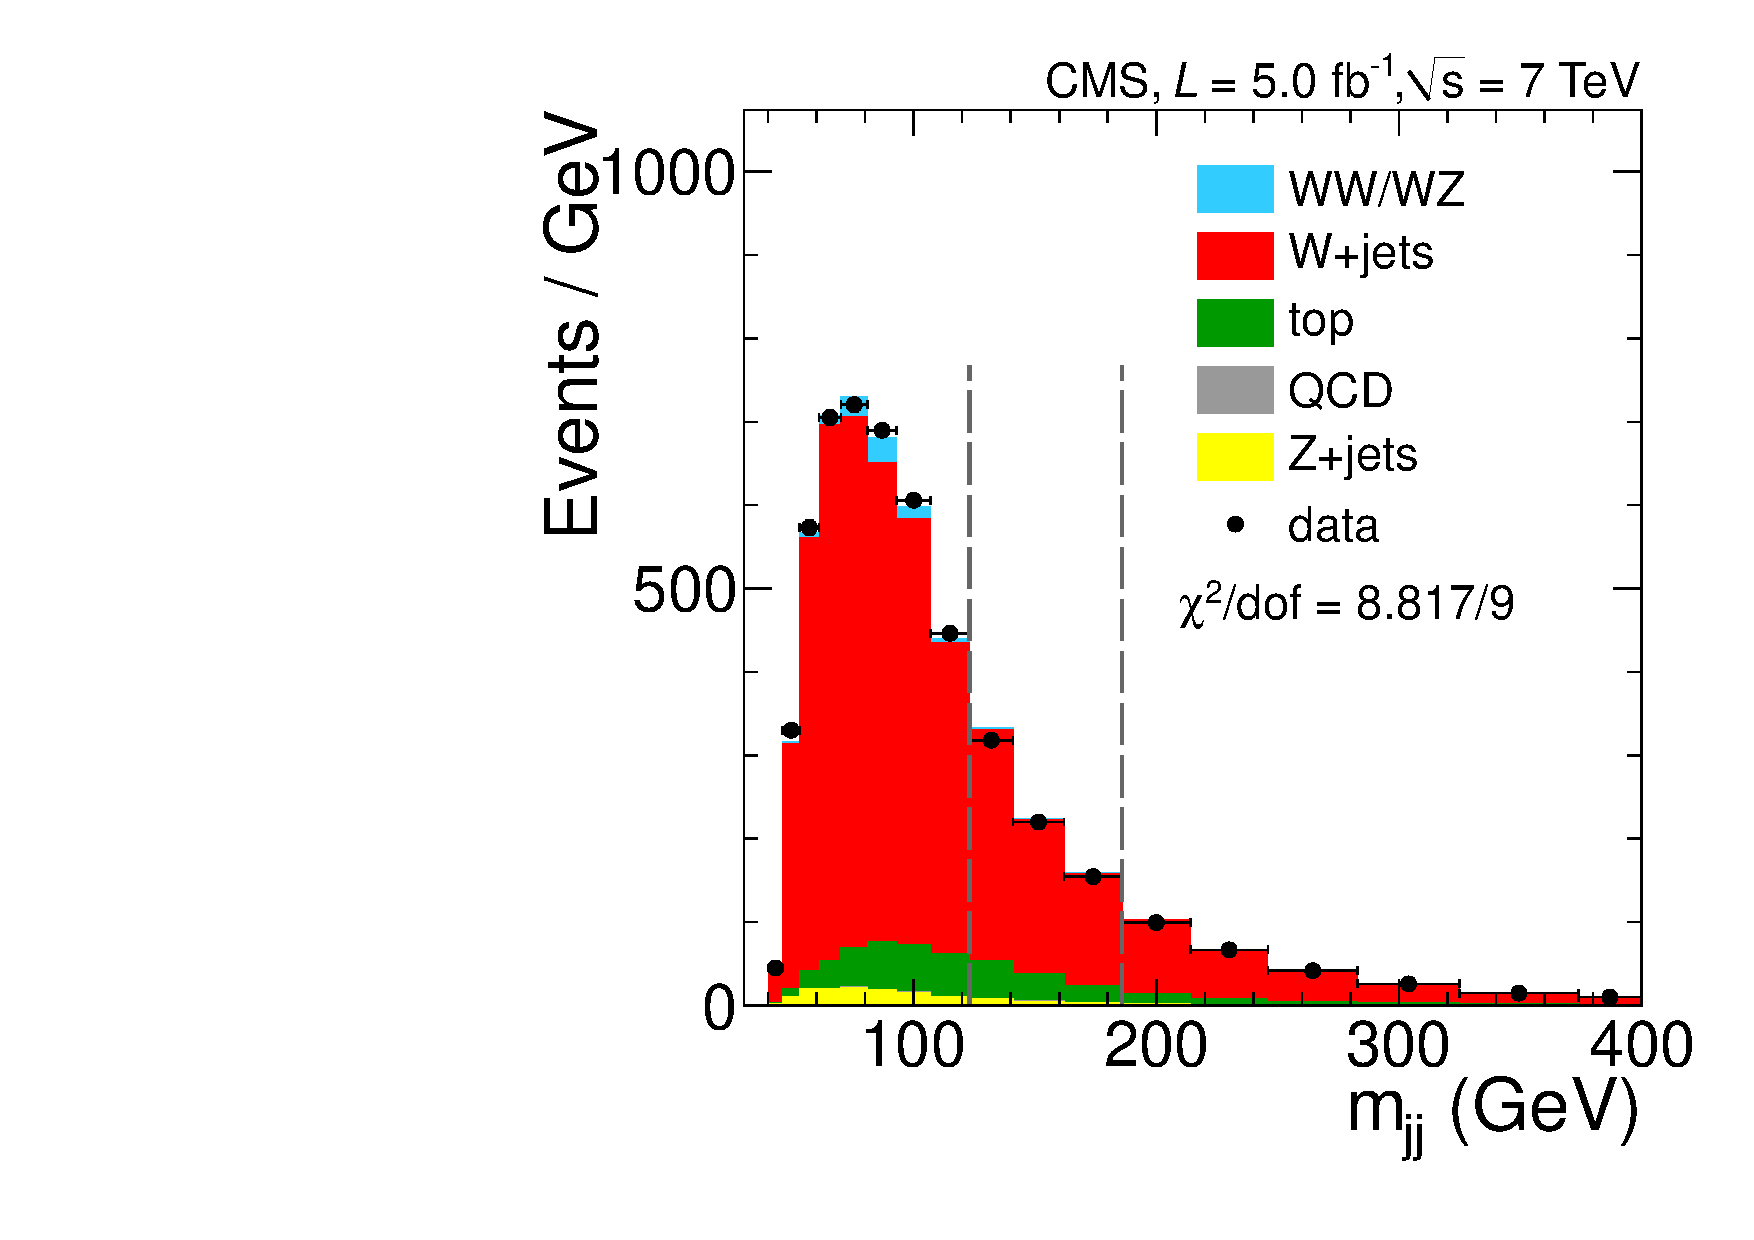
\includegraphics[width=0.49\textwidth]{figs/Wjj_Mjj_Muon_2jets_Stacked.pdf}
    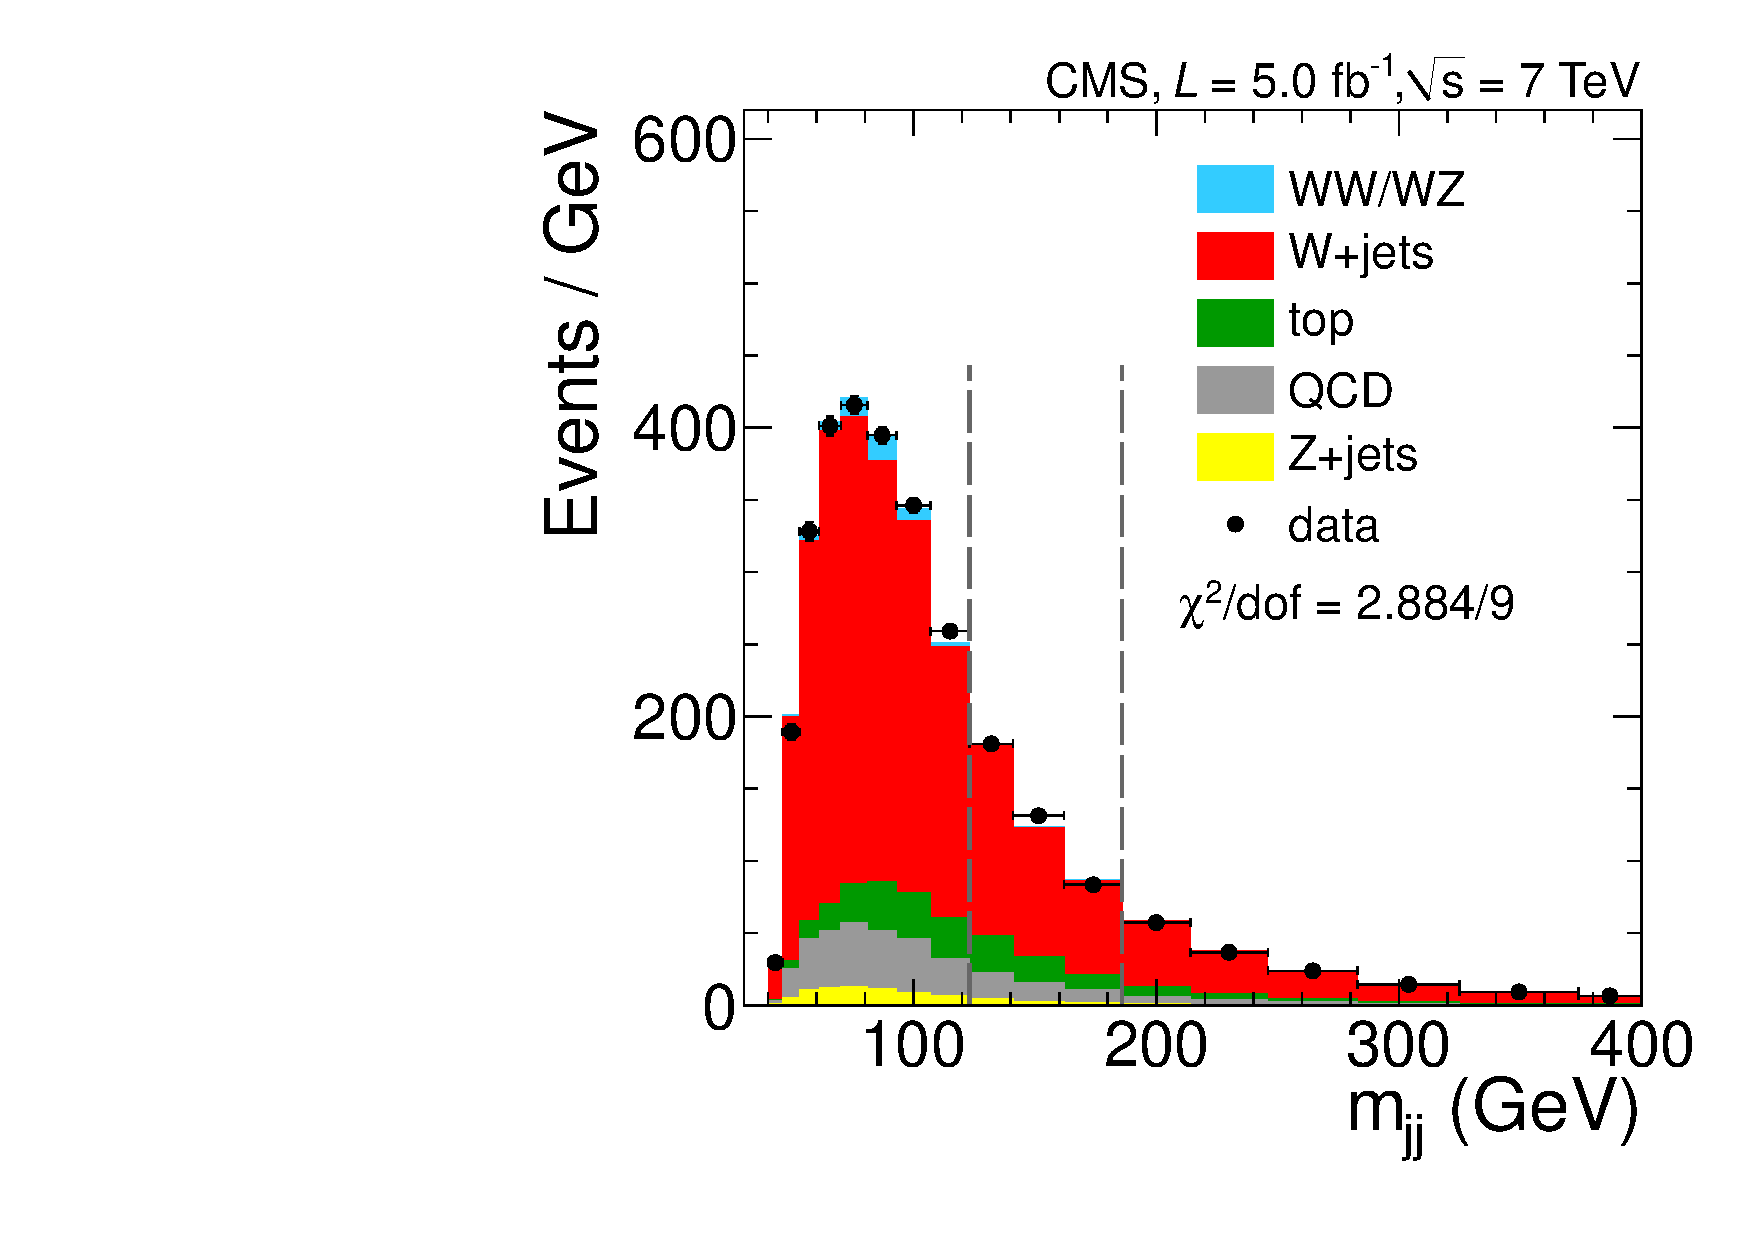
\includegraphics[width=0.49\textwidth]{figs/Wjj_Mjj_Electron_2jets_Stacked.pdf}
    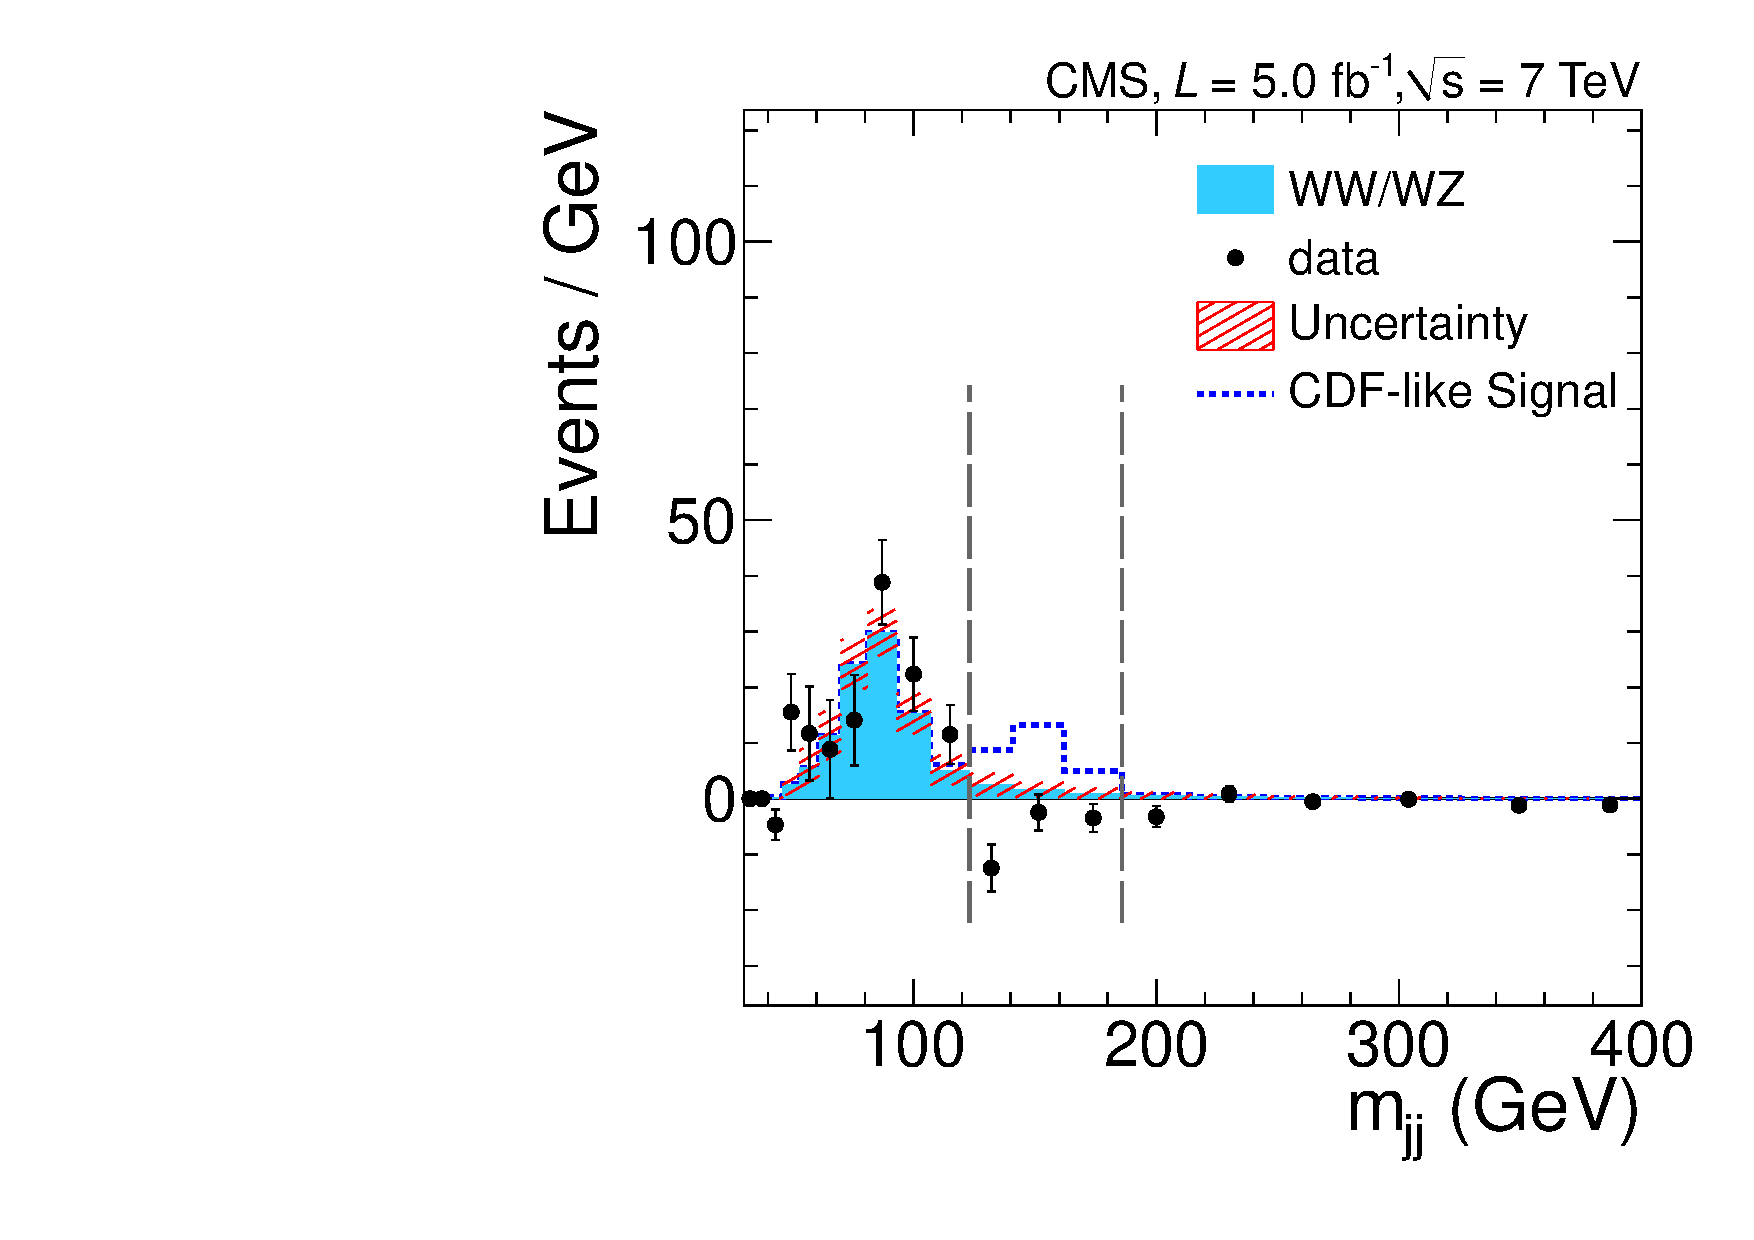
\includegraphics[width=0.49\textwidth]{figs/Wjj_Mjj_Muon_2jets_Subtracted.pdf}
    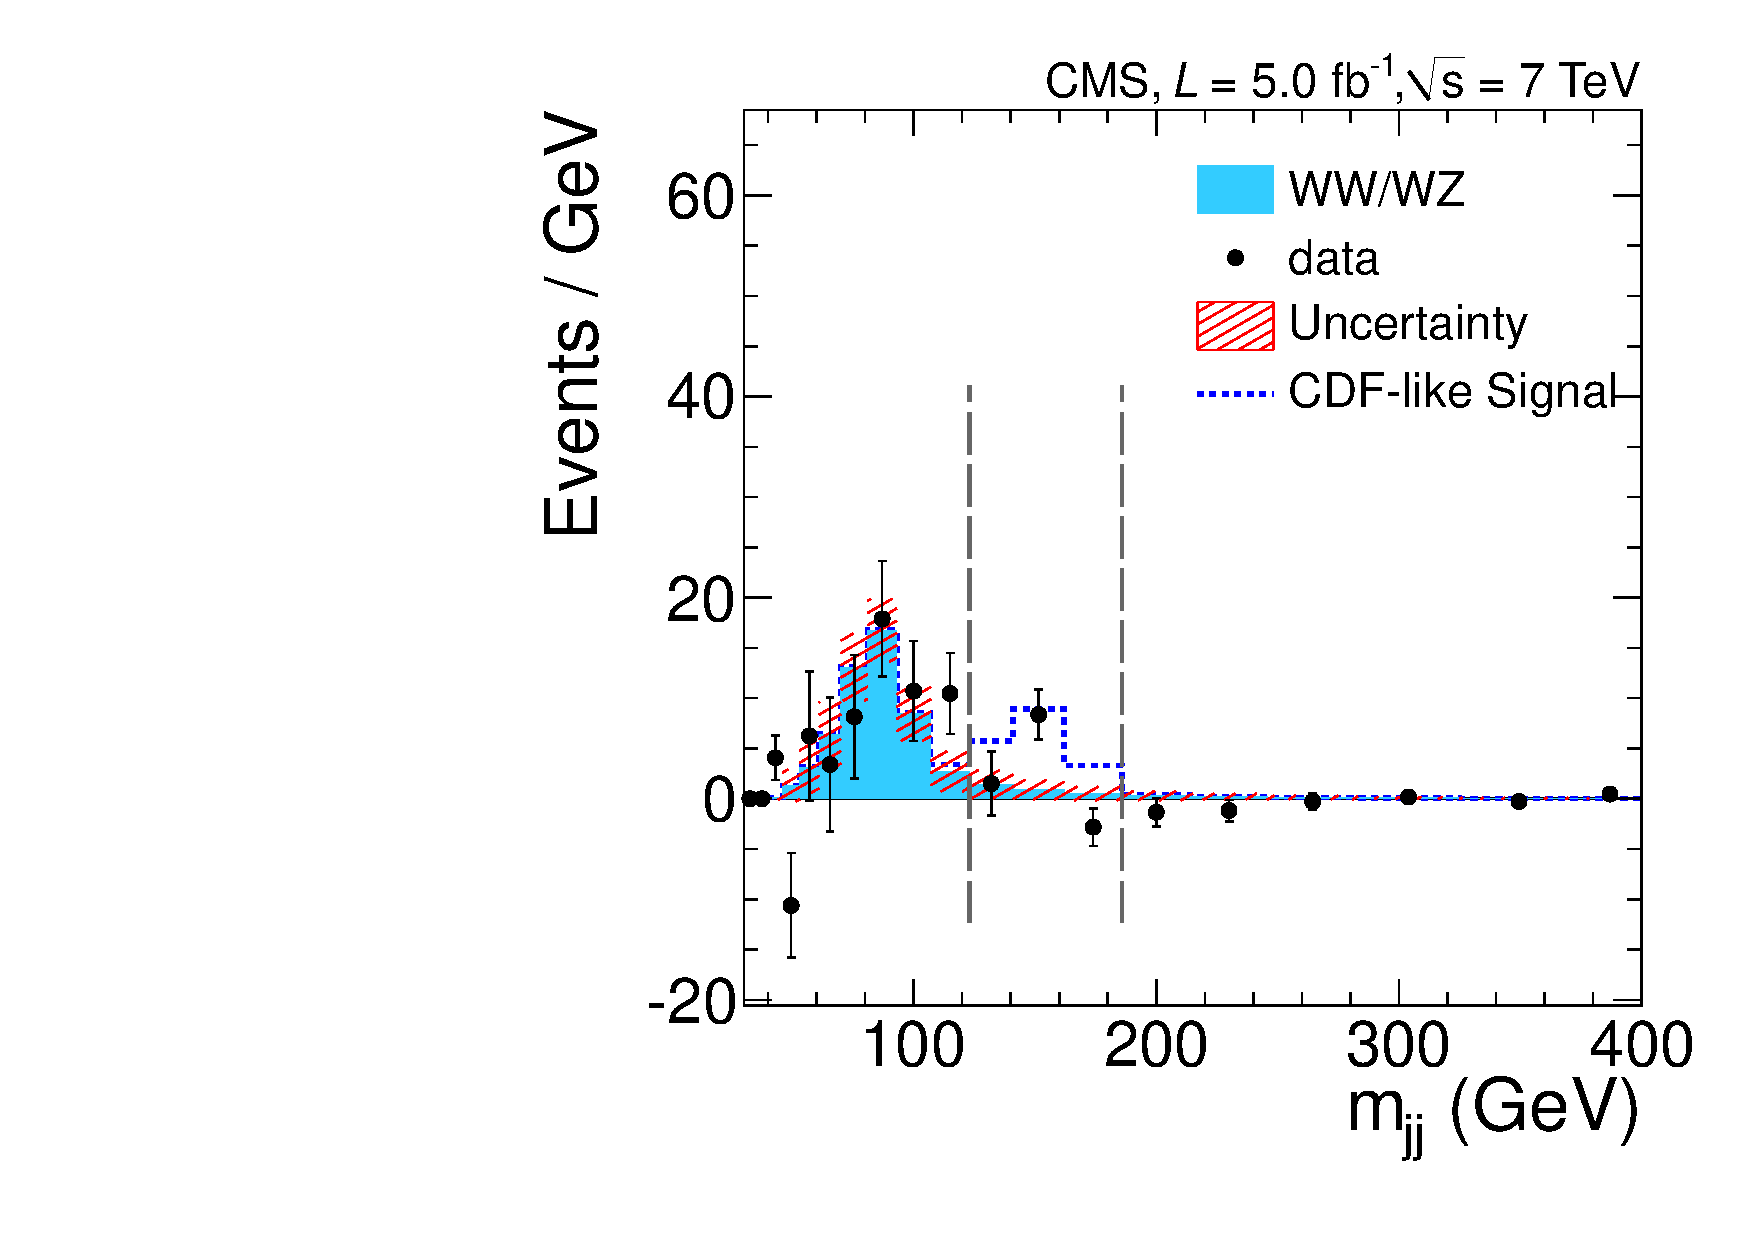
\includegraphics[width=0.49\textwidth]{figs/Wjj_Mjj_Electron_2jets_Subtracted.pdf}
    \caption{(upper row) Distribution of the invariant mass spectrum of the 
 two jets observed in data in muon plus 2 jets (left) 
 and electron plus 2 jets (right) categories. 
 Overlaid are the template distributions used 
 in the likelihood fit to the measured \mjj distibution, with their 
 relative normalization as obtained from the fit.              
 The region between the vertical dotted lines is excluded in the fit.       
 Depicted is the number of events per GeV, \textit{i.e.}, the raw event count can be obtained by
 multiplying with the bin width.                              
 (lower row) The same distribution after subtraction of all SM components   
 except the electroweak diboson WW/WZ. 
 Error bars correspond to the statistical uncertainty. 
 The band represents the systematic uncertainty in the sum of the SM components. 
}
\end{figure}





\begin{figure}[h!]
  {\centering
    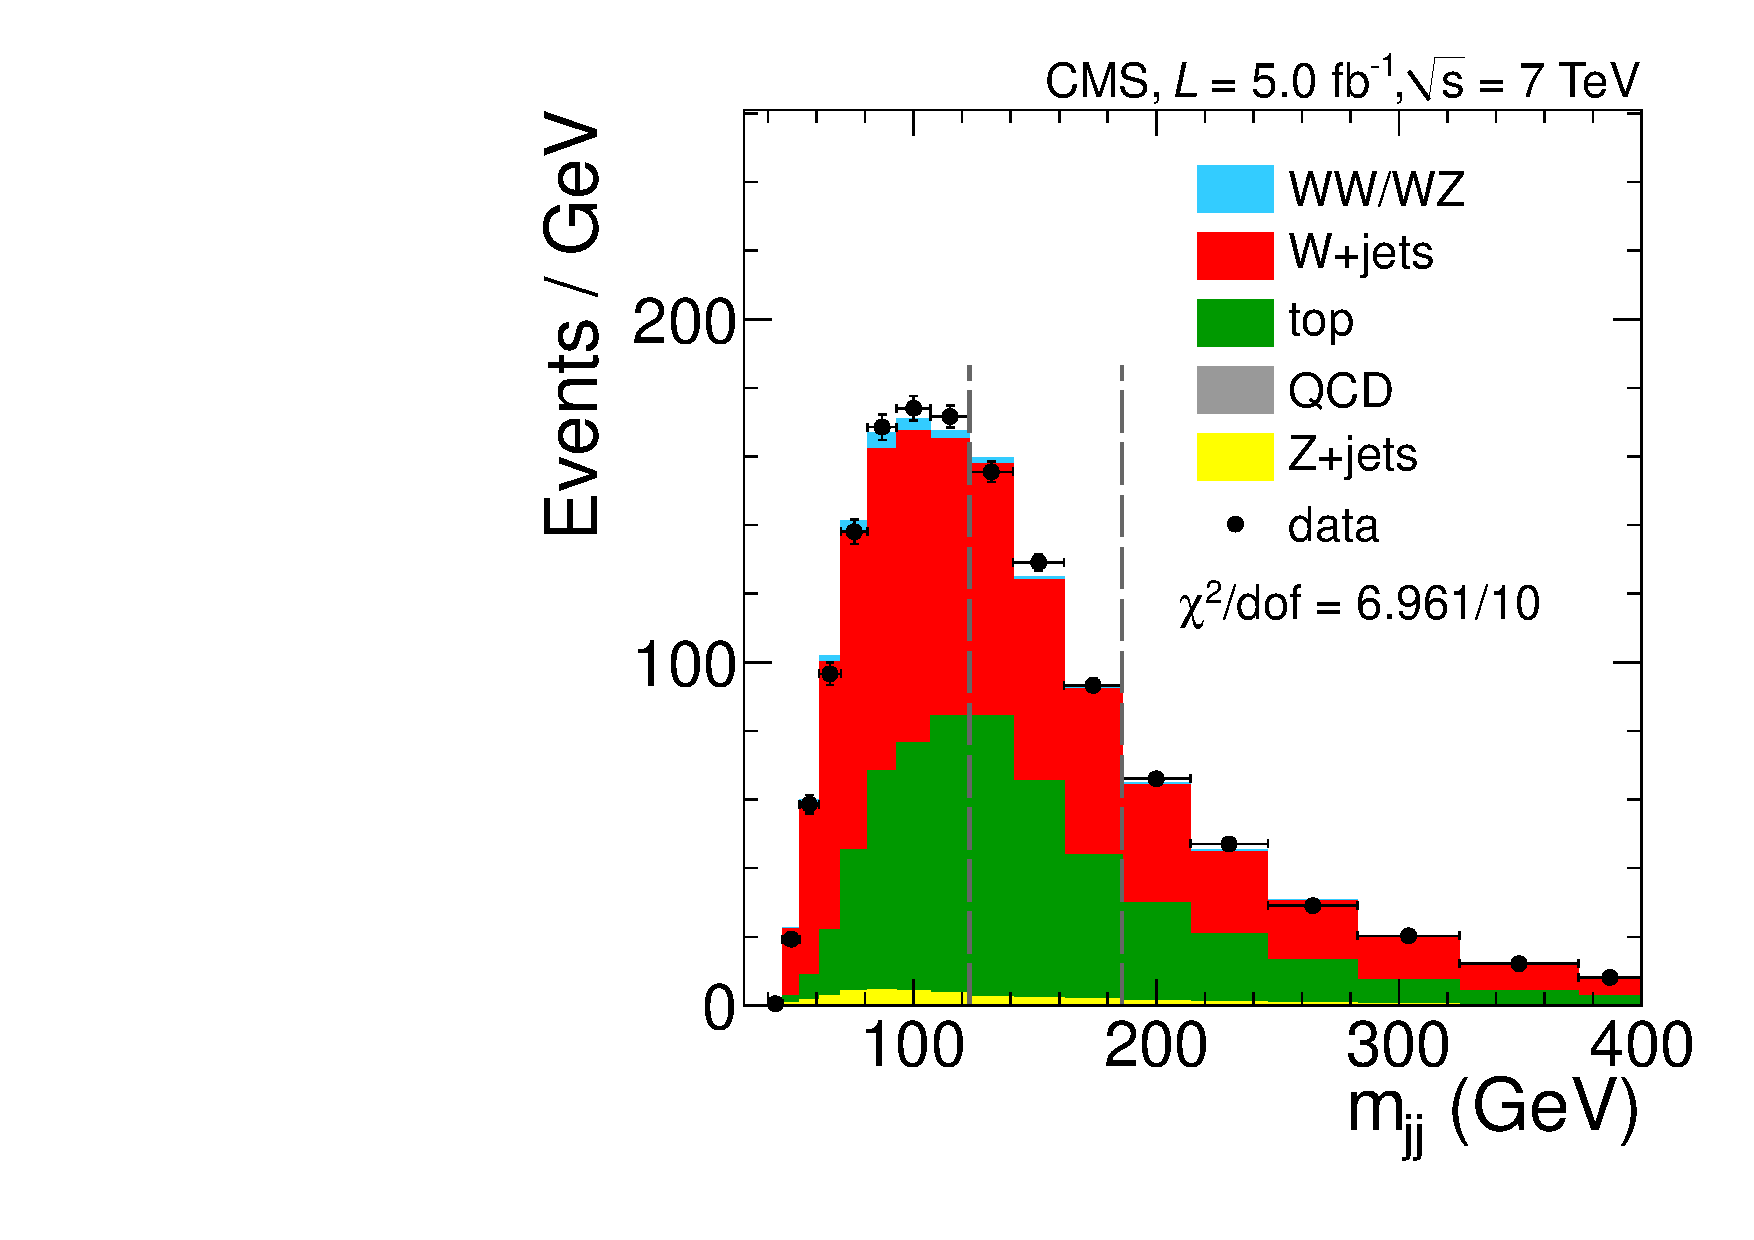
\includegraphics[width=0.49\textwidth]{figs/Wjj_Mjj_Muon_3jets_Stacked.pdf}
    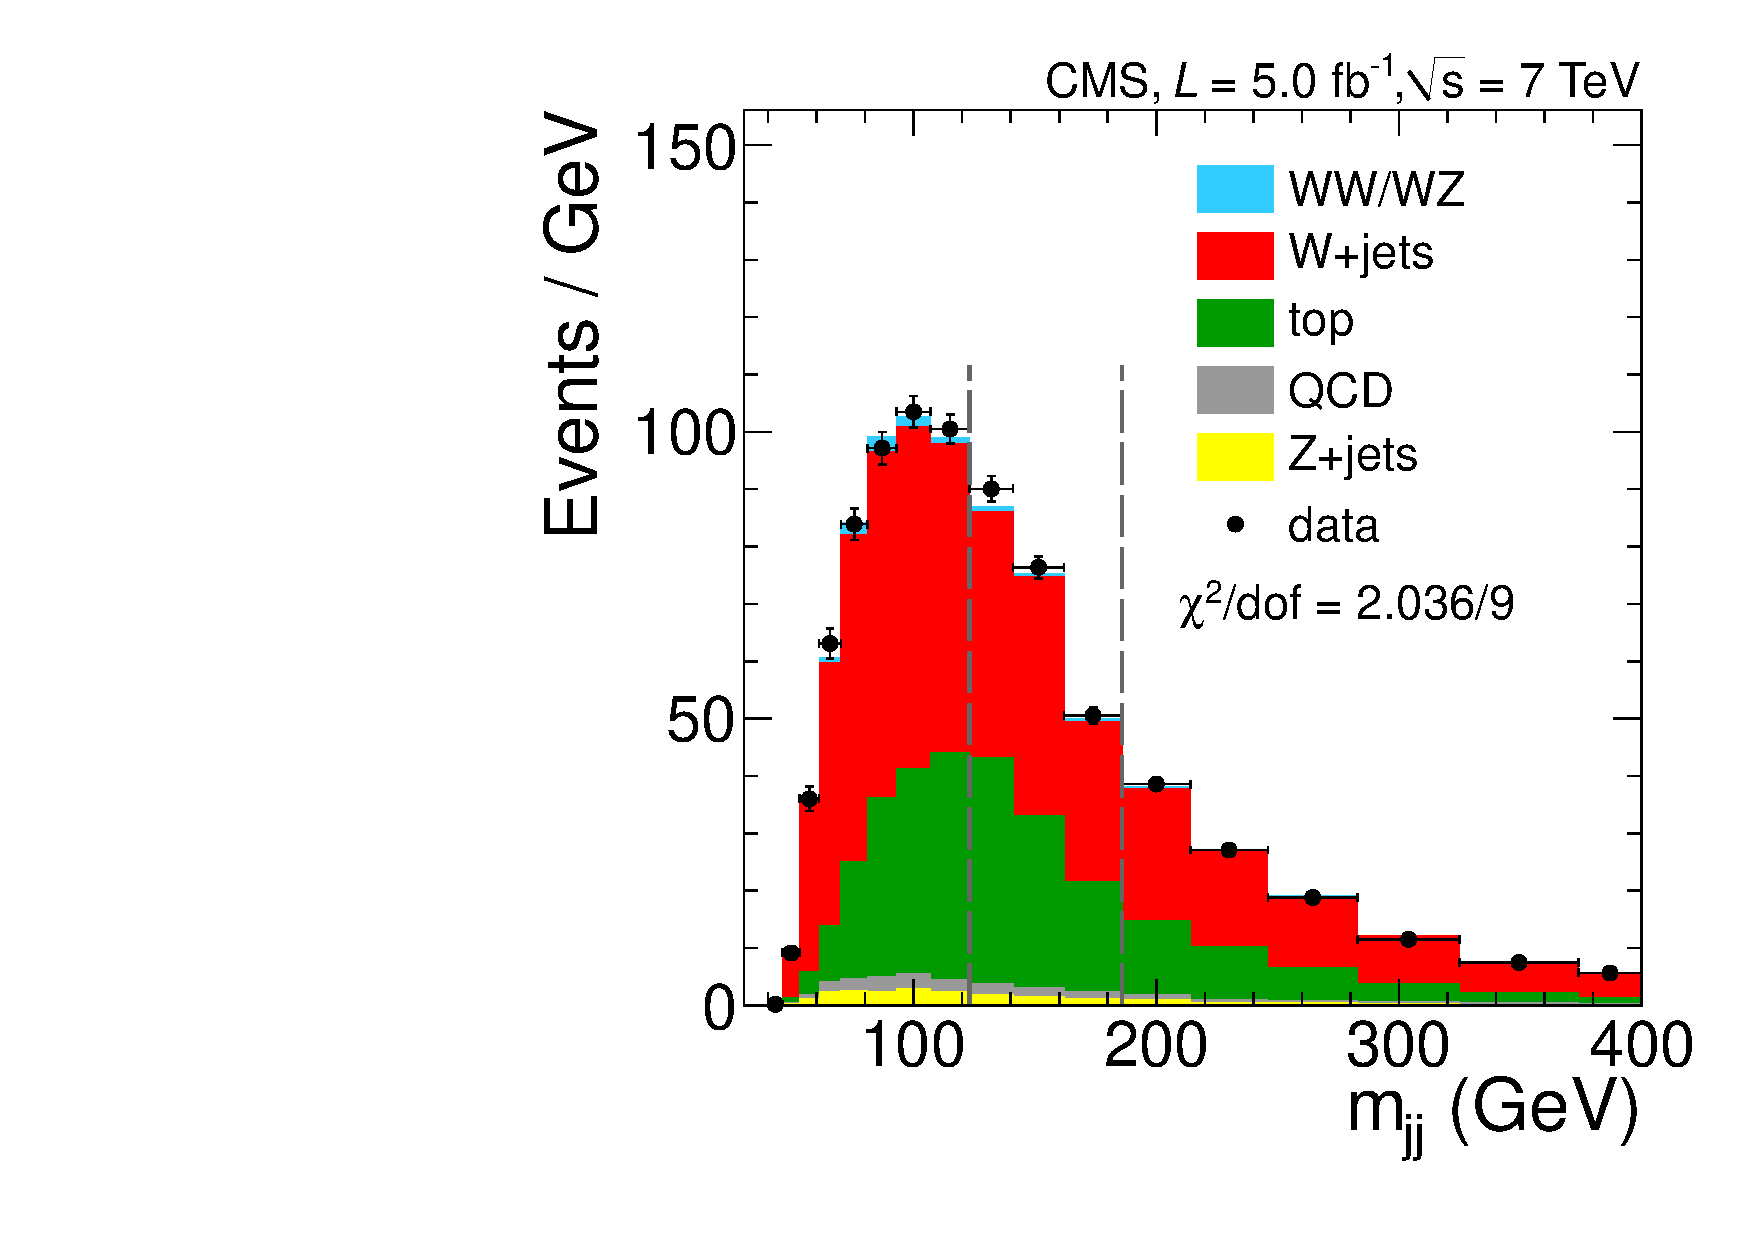
\includegraphics[width=0.49\textwidth]{figs/Wjj_Mjj_Electron_3jets_Stacked.pdf}
    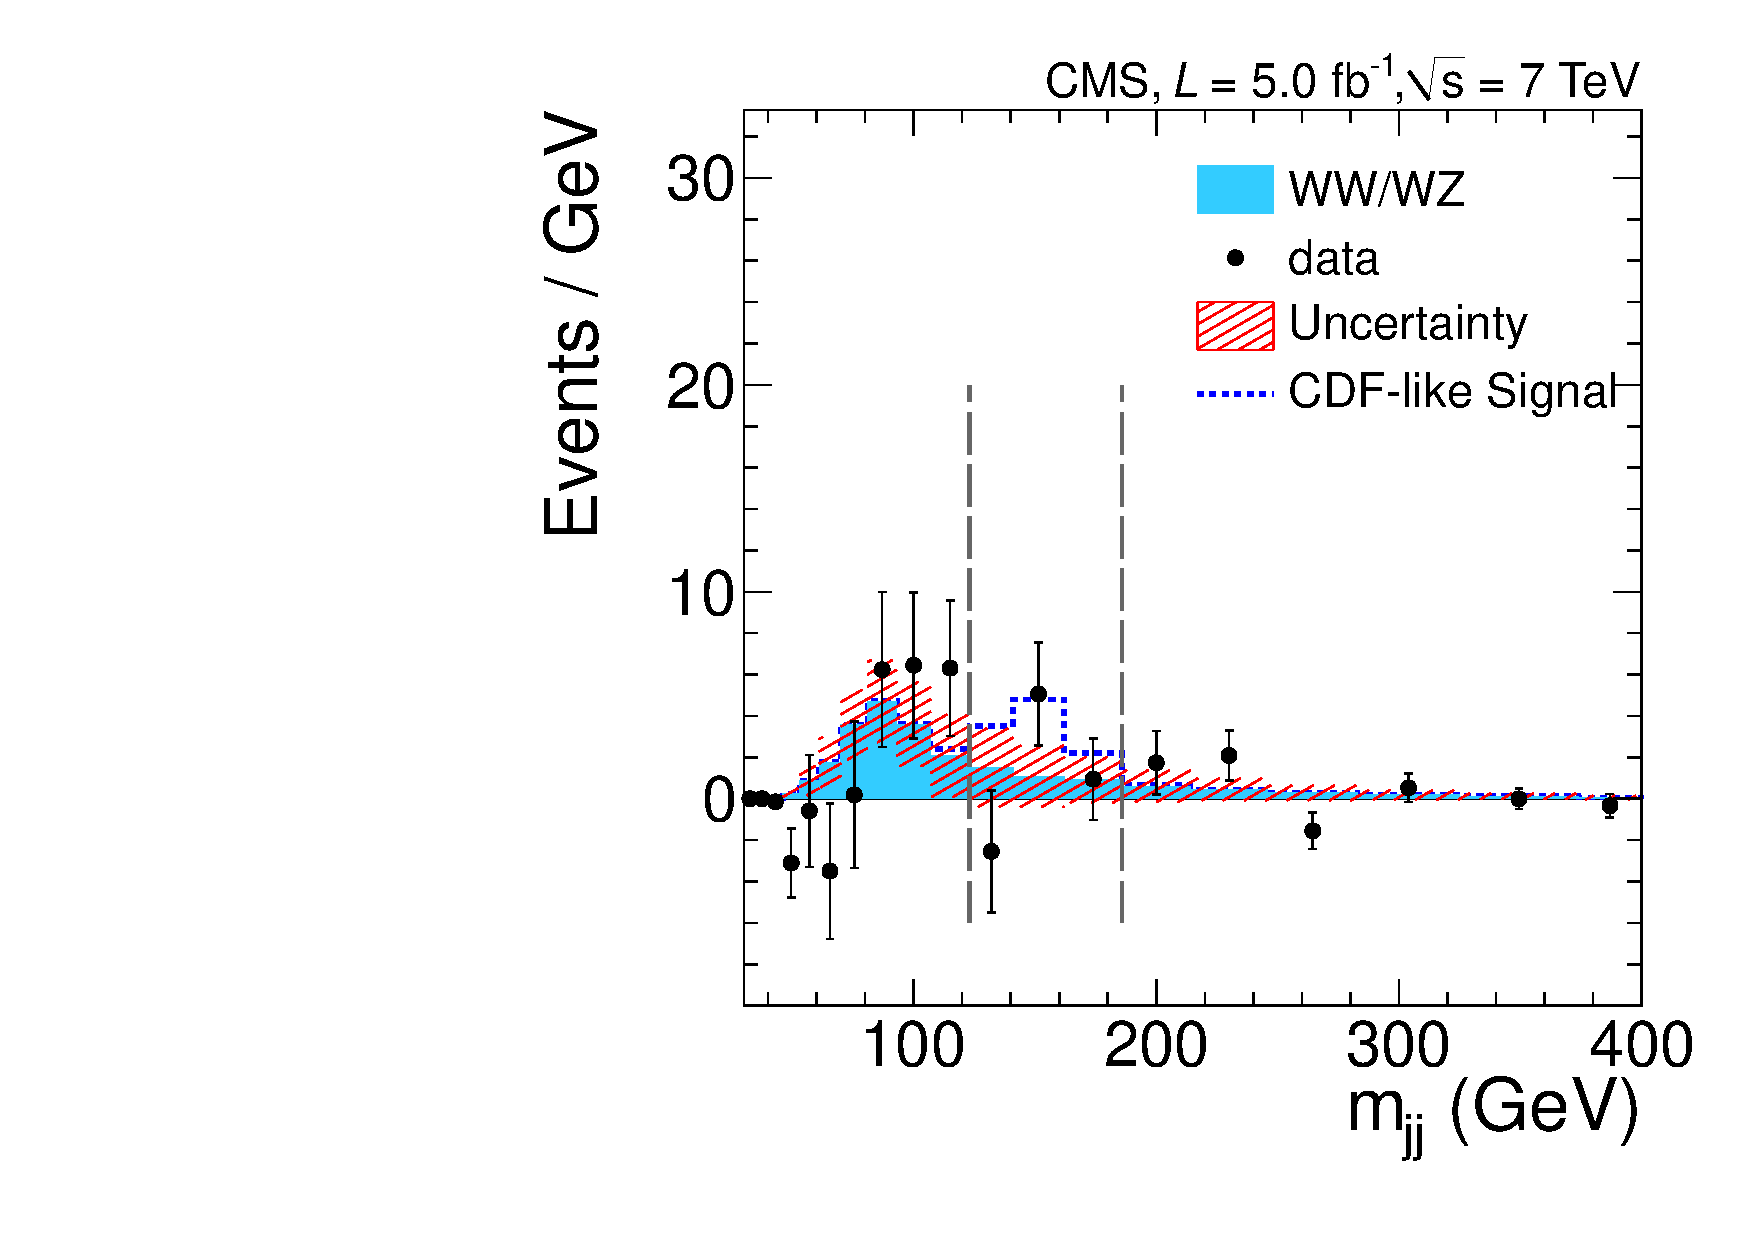
\includegraphics[width=0.49\textwidth]{figs/Wjj_Mjj_Muon_3jets_Subtracted.pdf}
    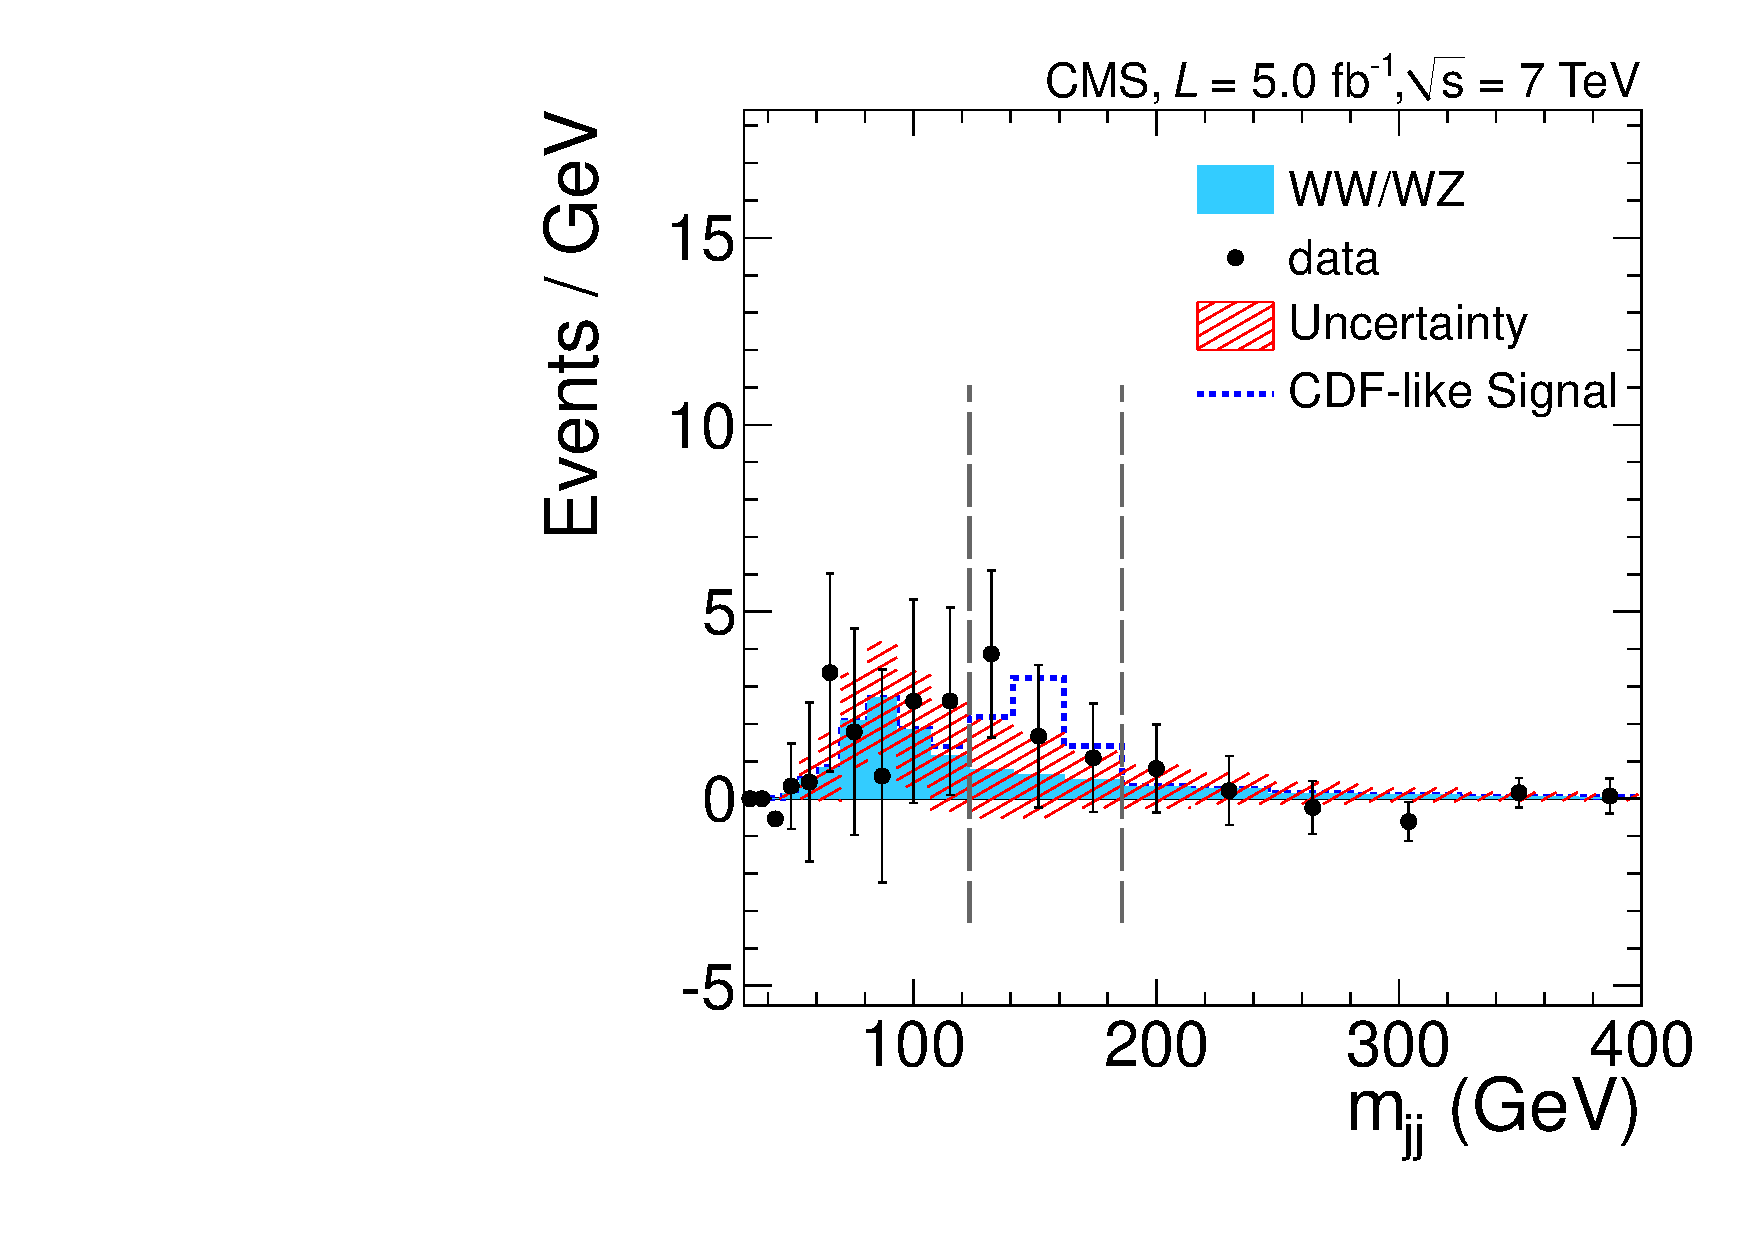
\includegraphics[width=0.49\textwidth]{figs/Wjj_Mjj_Electron_3jets_Subtracted.pdf}
    \caption{(upper row) Distribution of the invariant mass spectrum of the 
 leading two jets observed in data in muon plus 3 jets (left) 
 and electron plus 3 jets (right) categories. 
 Overlaid are the template distributions used 
 in the likelihood fit to the measured \mjj distibution, with their 
 relative normalization as obtained from the fit.              
 The region between the vertical dotted lines is excluded in the fit.       
 Depicted is the number of events per GeV, \textit{i.e.}, the raw event count can be obtained by
 multiplying with the bin width.                              
 (lower row) The same distribution after subtraction of all SM components   
 except the electroweak diboson WW/WZ. 
 Error bars correspond to the statistical uncertainty. 
 The band represents the systematic uncertainty in the sum of the SM components. 
}
\end{figure}




\begin{figure}[h!t]
  {\centering
    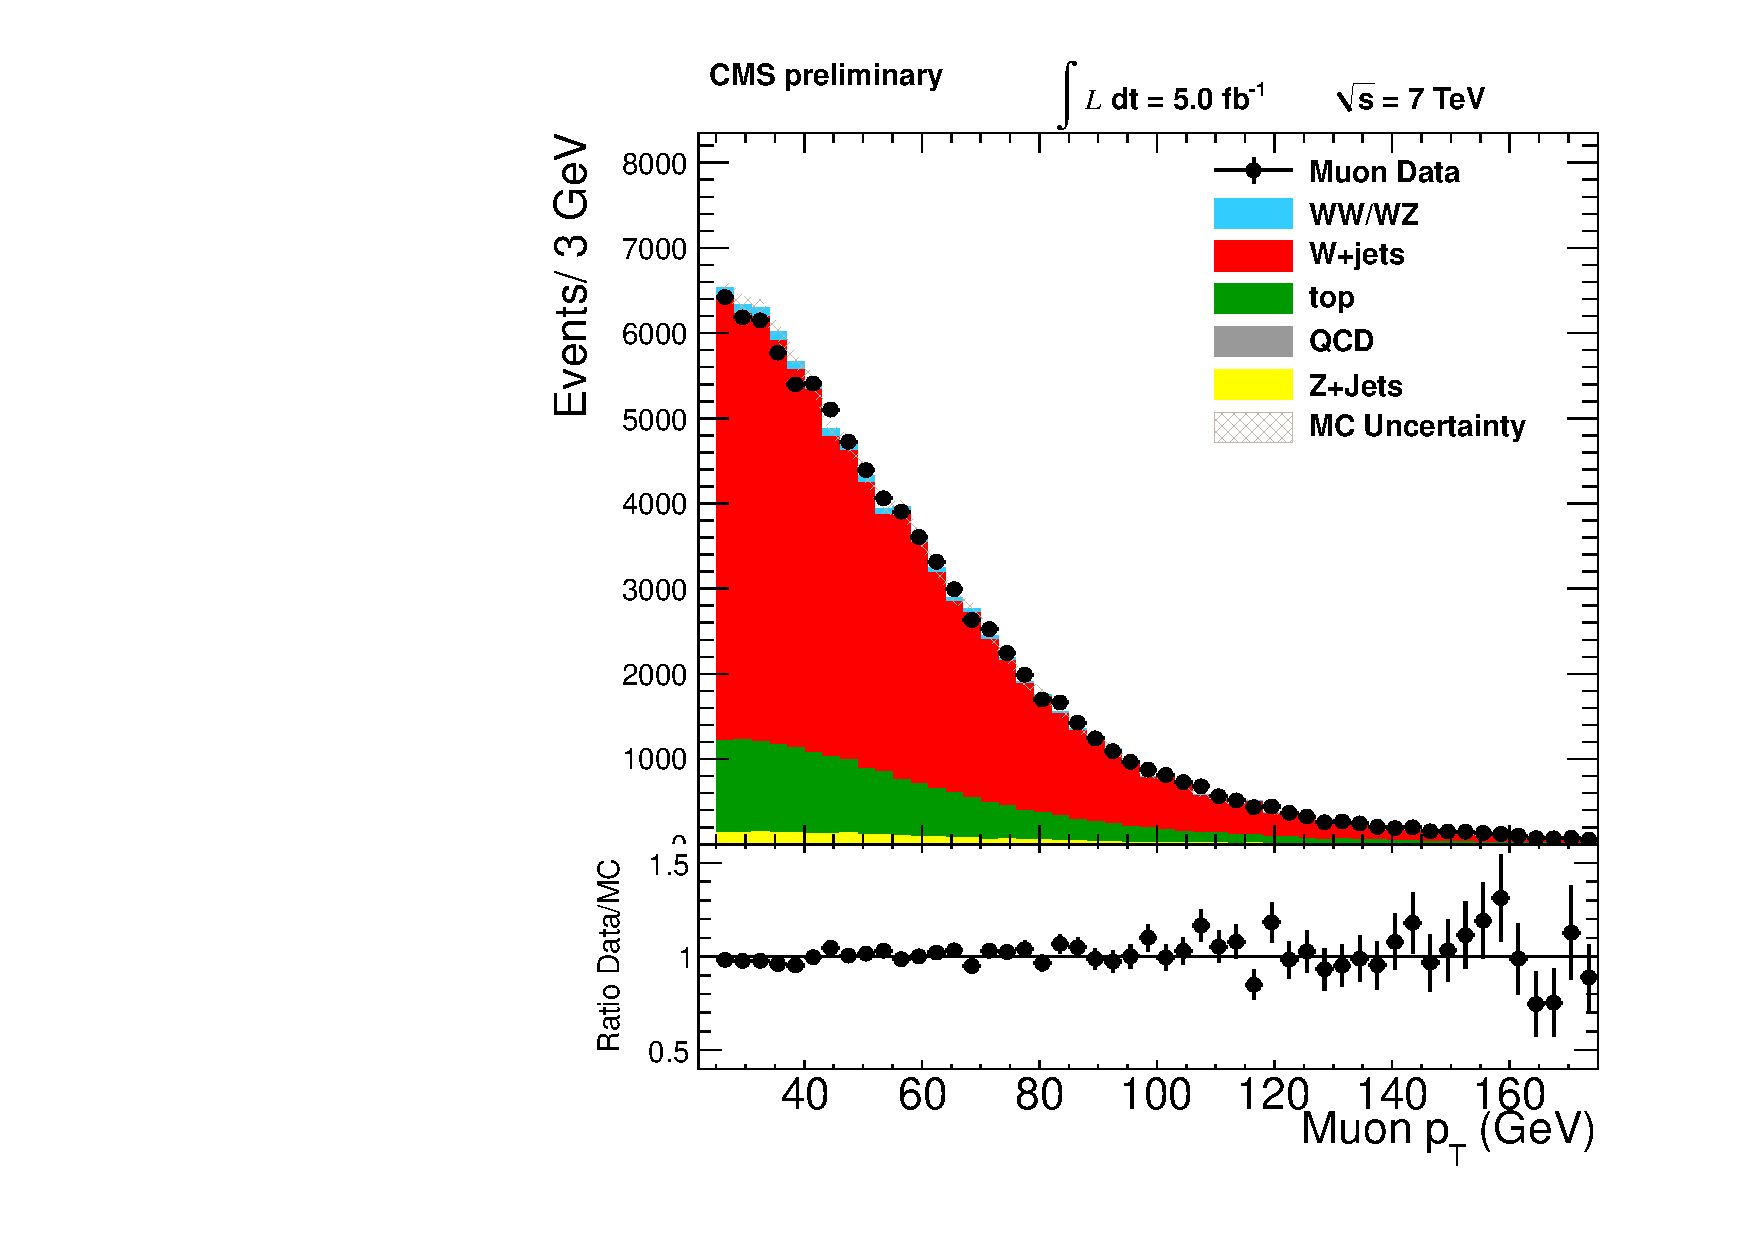
\includegraphics[width=0.3\textwidth]{figs/mu_W_muon_pt.pdf}
    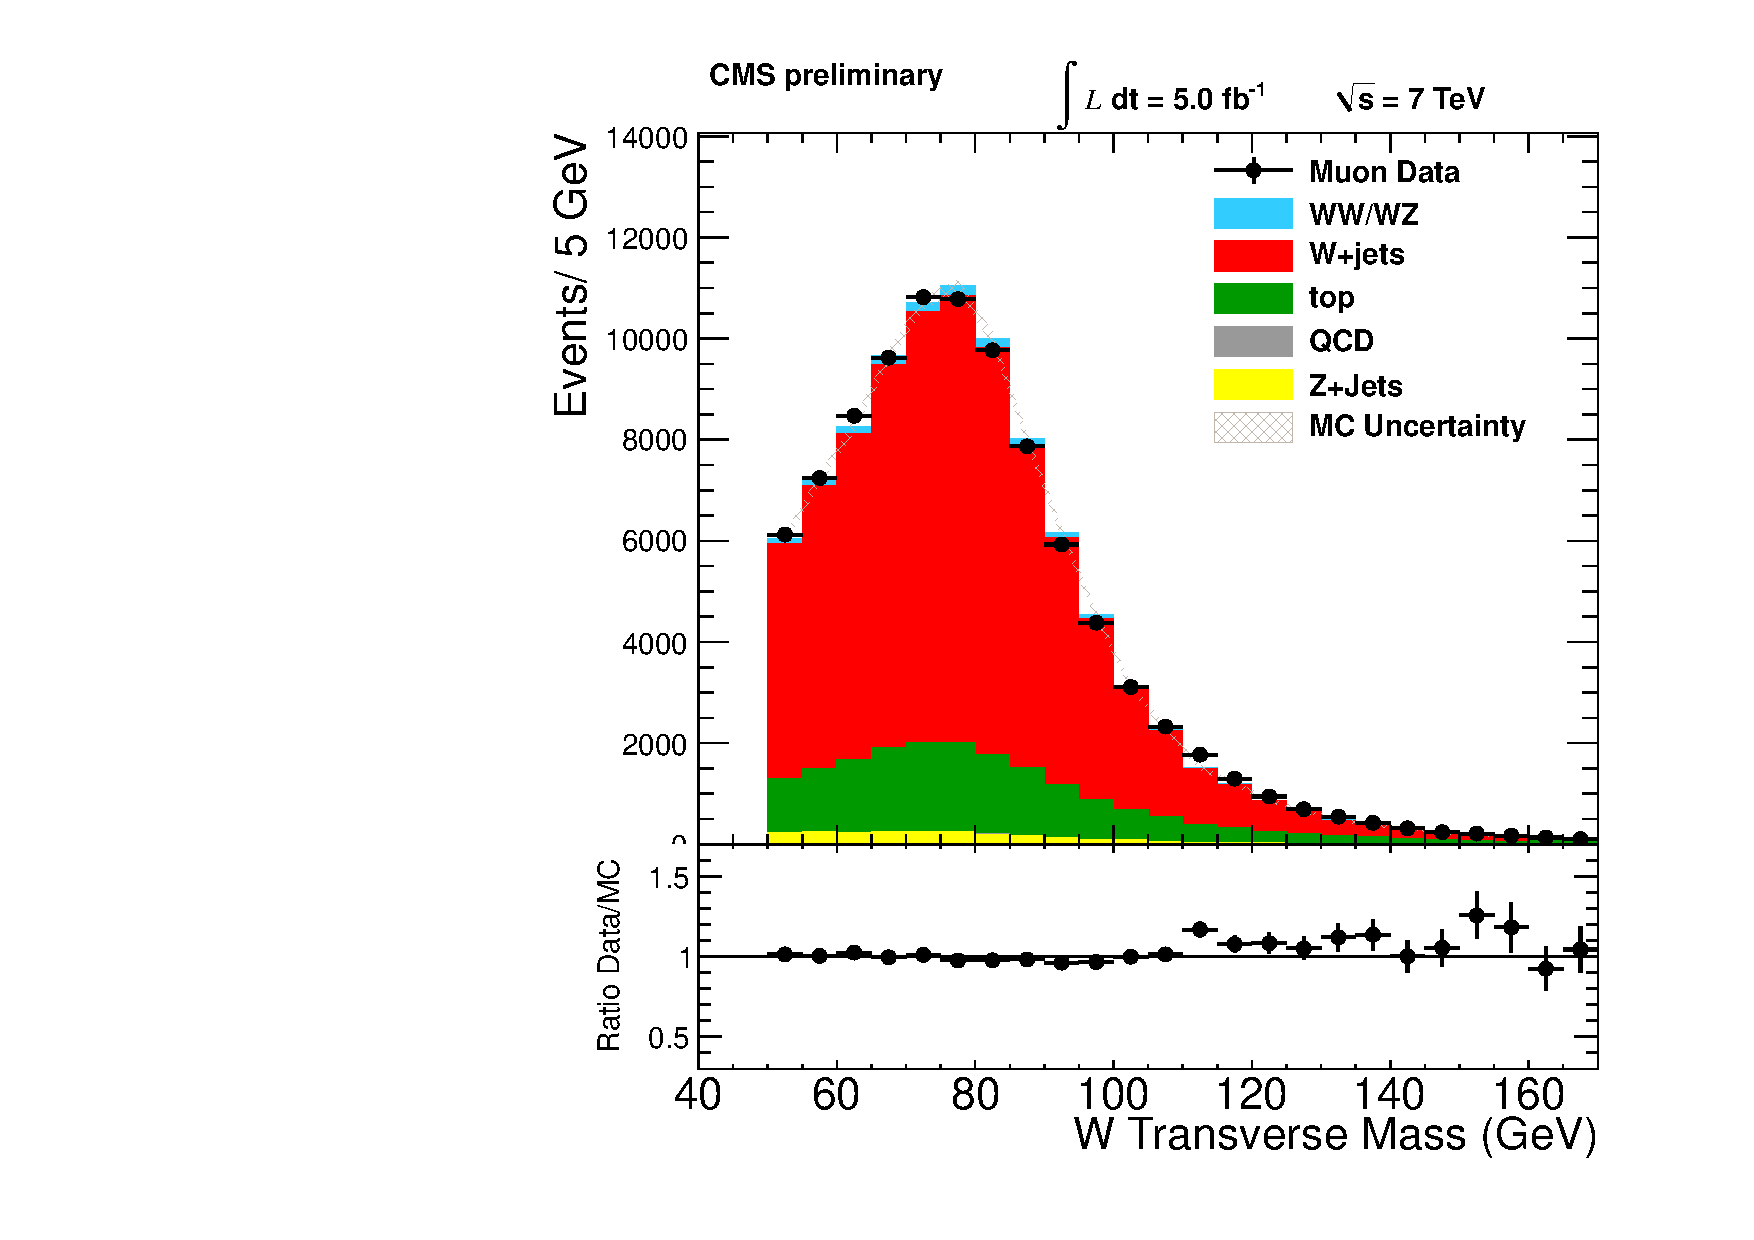
\includegraphics[width=0.3\textwidth]{figs/mu_W_mt.pdf}
    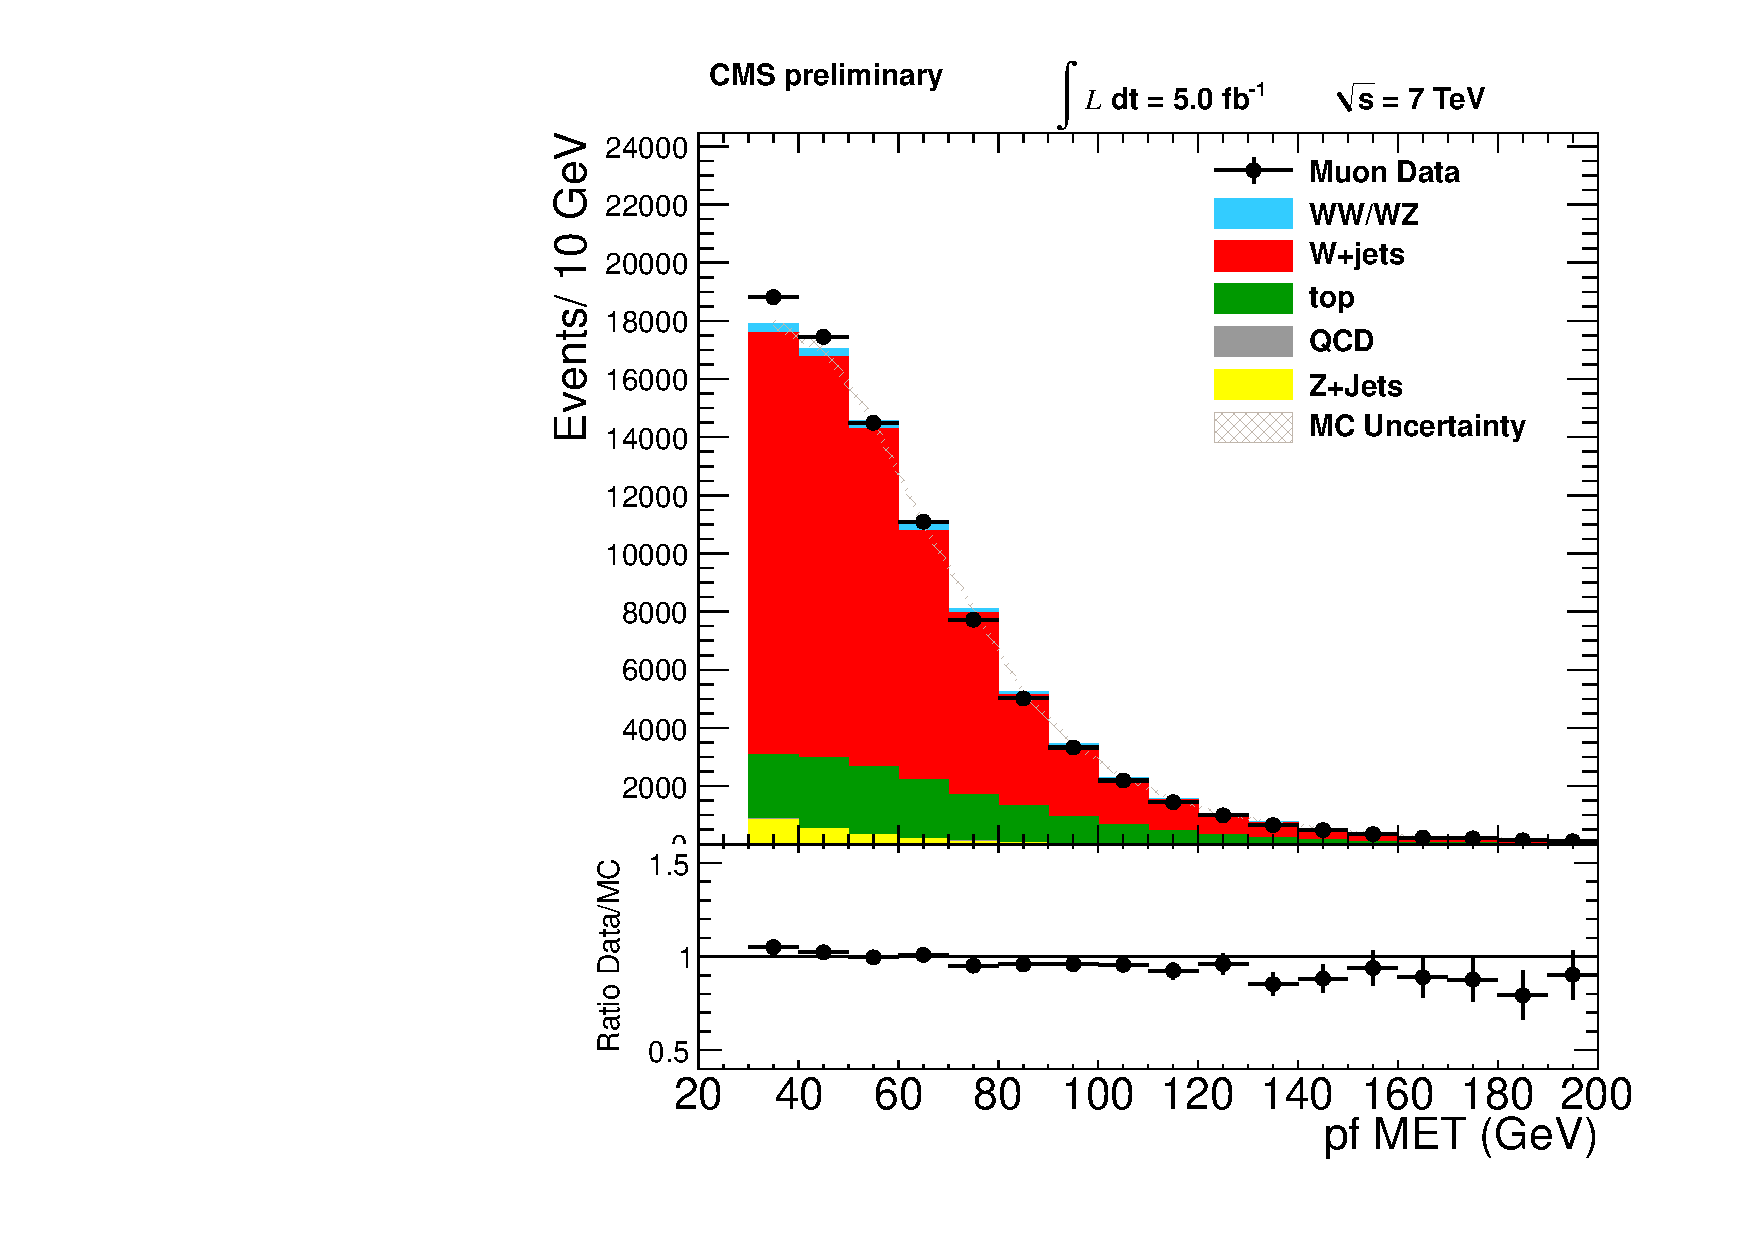
\includegraphics[width=0.3\textwidth]{figs/mu_event_met_pfmet.pdf}
    \caption{Comparison of the distributions in data and MC for the muon plus jets event sample after event selection 
    (left) of the transverse momentum of the muon candidate, (middle) of the transverse momentum of the 
    reconstructed W candidate, (right) of the missing transverse energy. The error bars on the data points are statistical only.
    The relative normalization of the various MC samples are taken from the result of the fit to the \mjj spectrum. 
%%The resulting
%%    MC histogram was normalized to the number of events in the data histogram.
    }}
\end{figure}


\begin{figure}[h!t]
  {\centering
    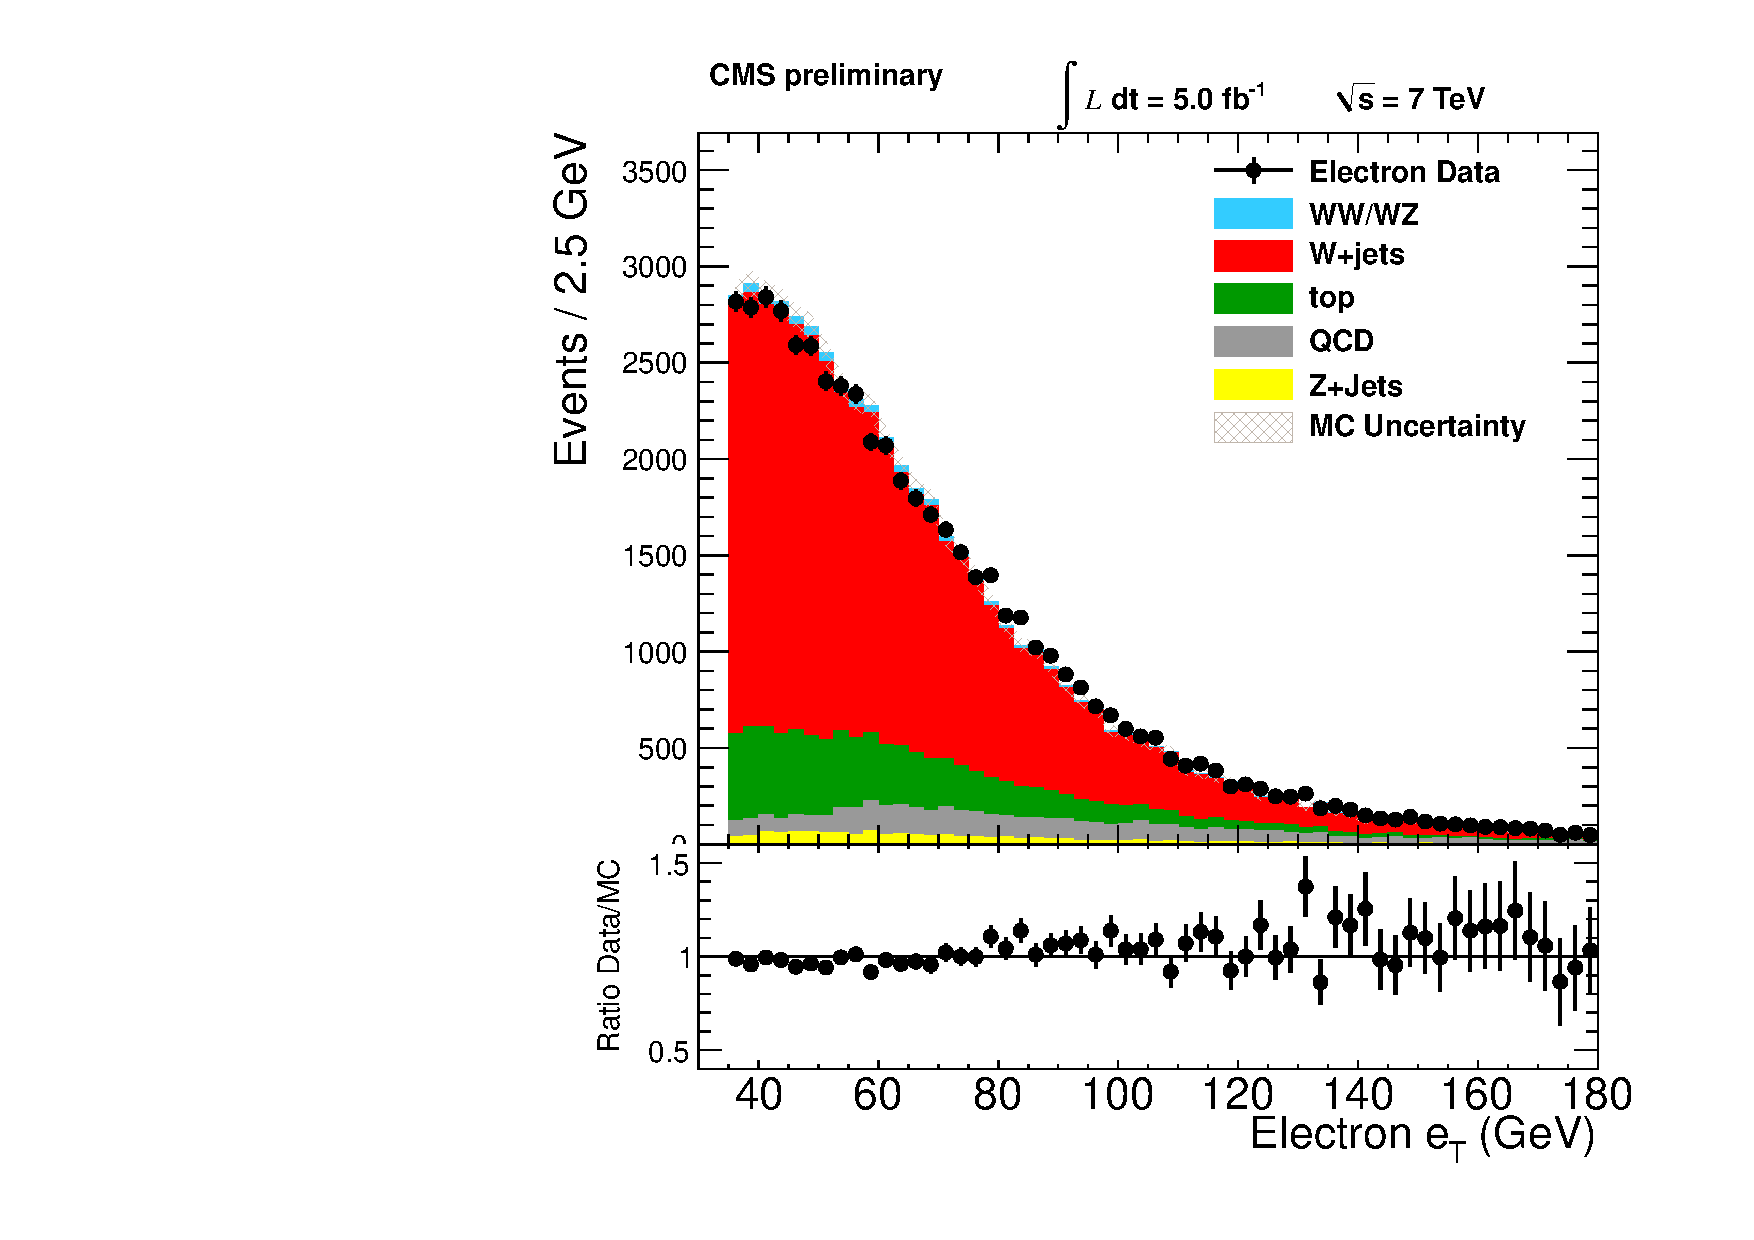
\includegraphics[width=0.3\textwidth]{figs/elec_W_electron_et.pdf}
    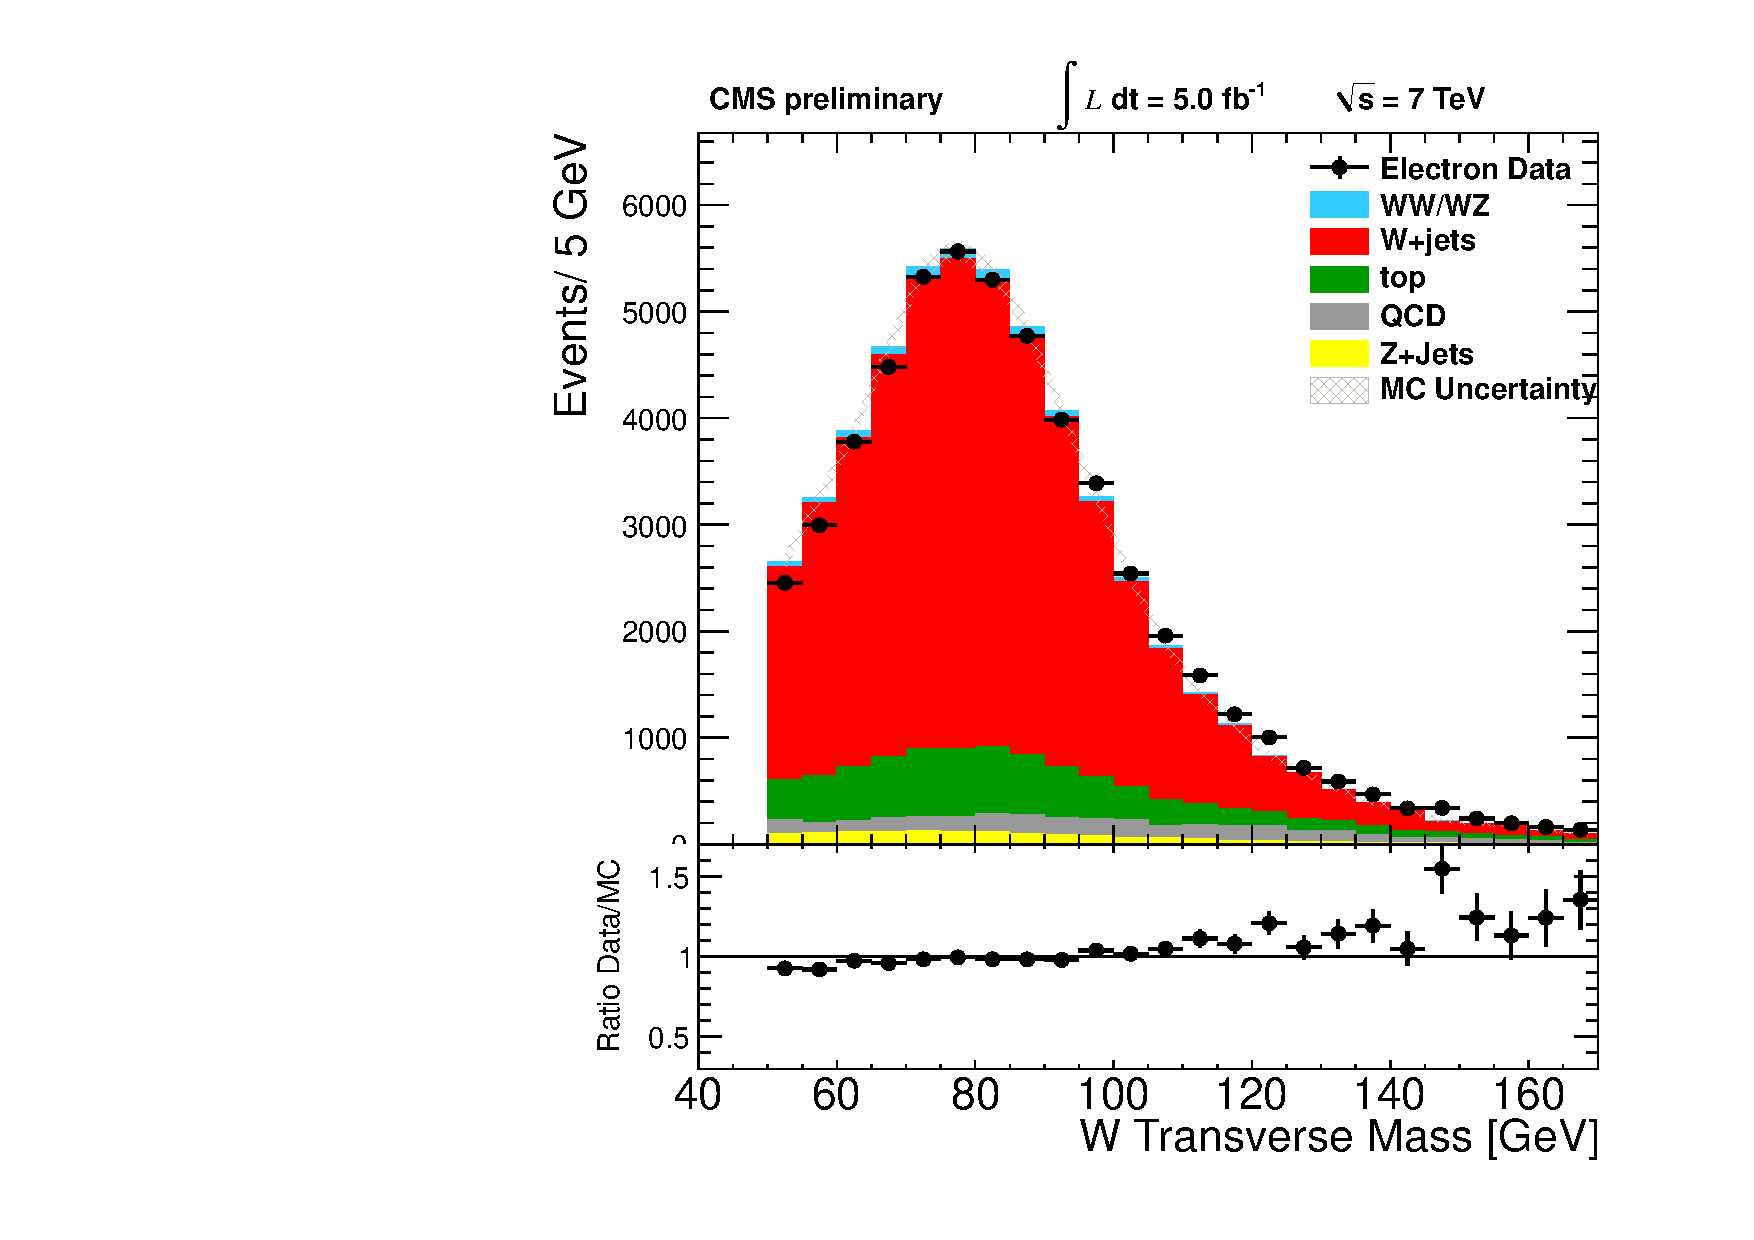
\includegraphics[width=0.3\textwidth]{figs/el_W_mt.pdf}
    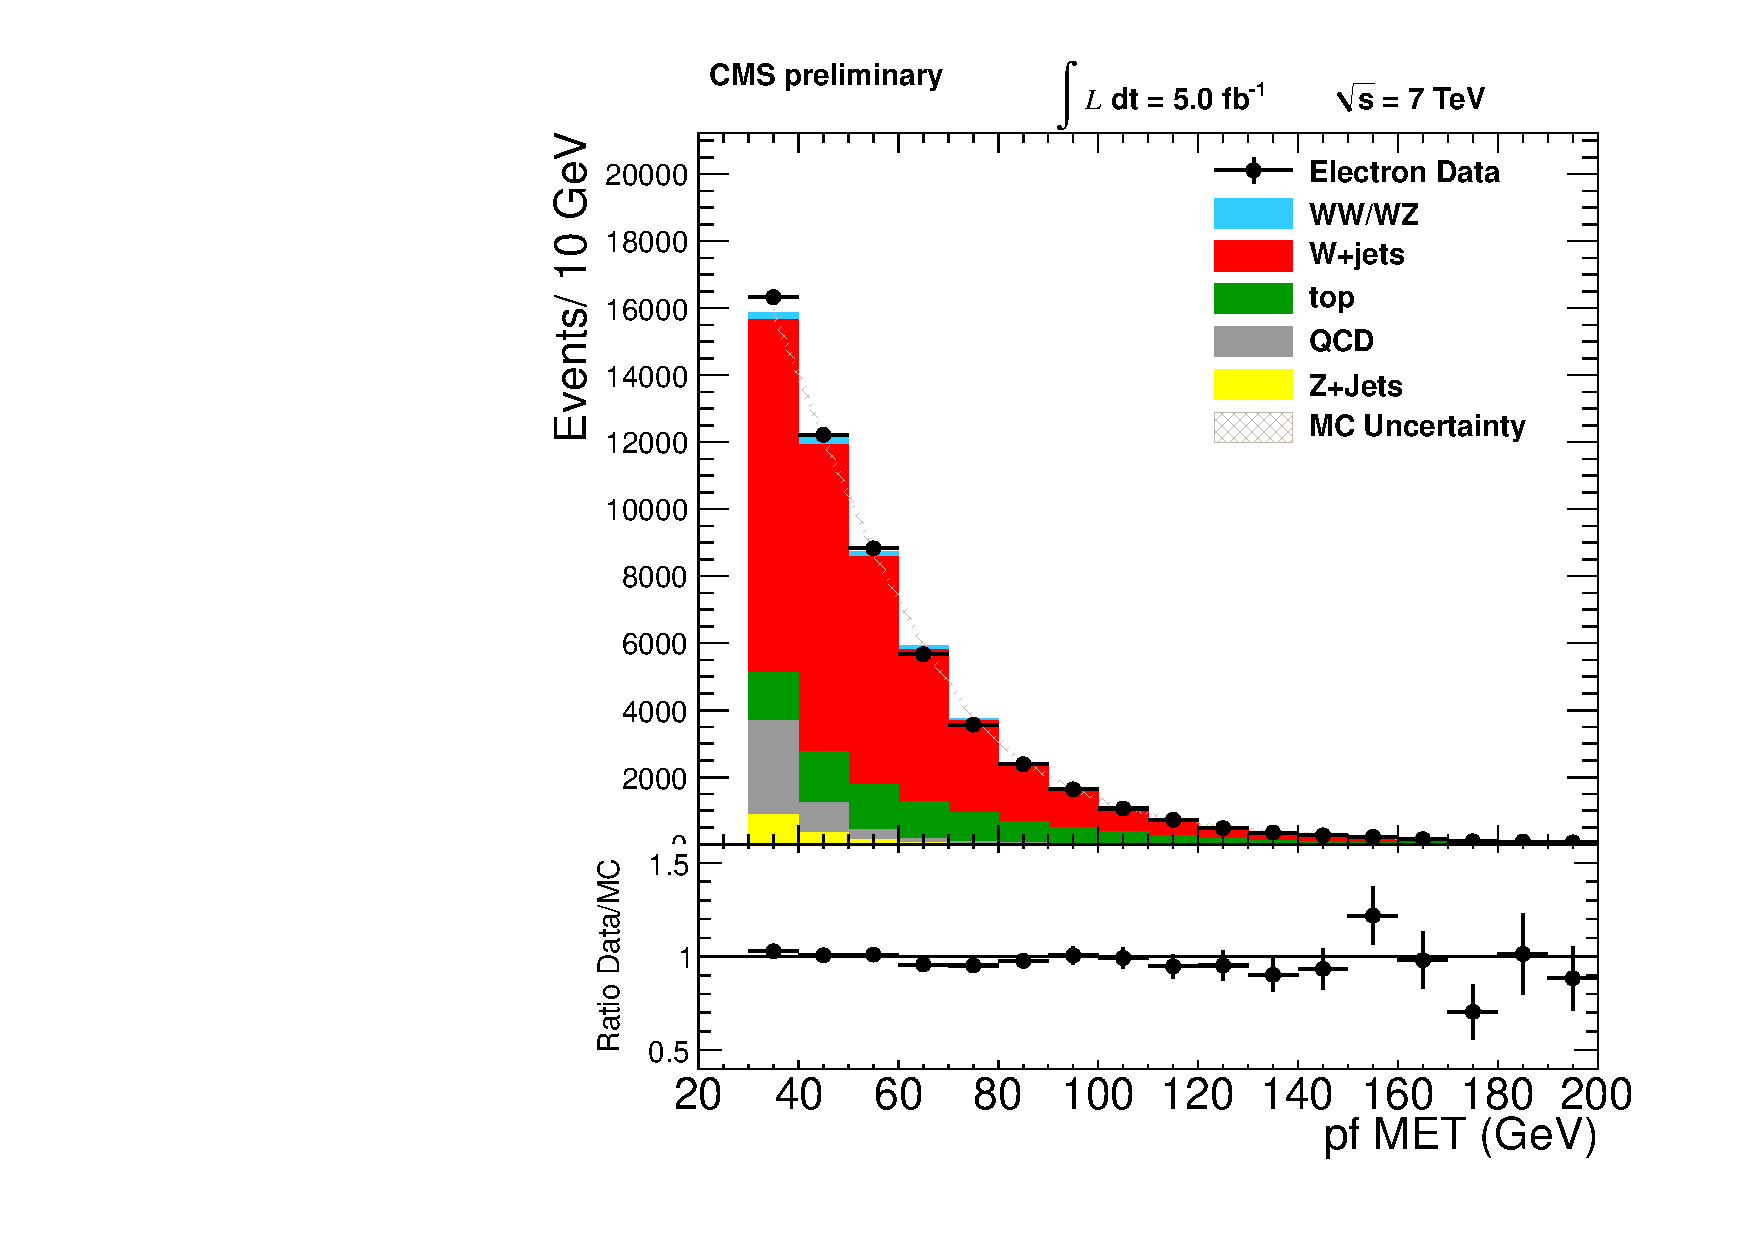
\includegraphics[width=0.3\textwidth]{figs/el_event_met_pfmet.pdf}
    \caption{Comparison of the distributions in data and MC for the electron plus jets event sample after event selection 
    (left) of the transverse energy of the electron candidate, (middle) of the transverse momentum of the 
    reconstructed W candidate, (right) of the missing transverse energy. The error bars on the data points are statistical only.
    The relative normalization of the various MC samples are taken from the result of the fit to the \mjj spectrum. 
%%The resulting
%%    MC histogram was normalized to the number of events in the data histogram.
      }}
\end{figure}



\begin{figure}[h!t]
  {\centering
    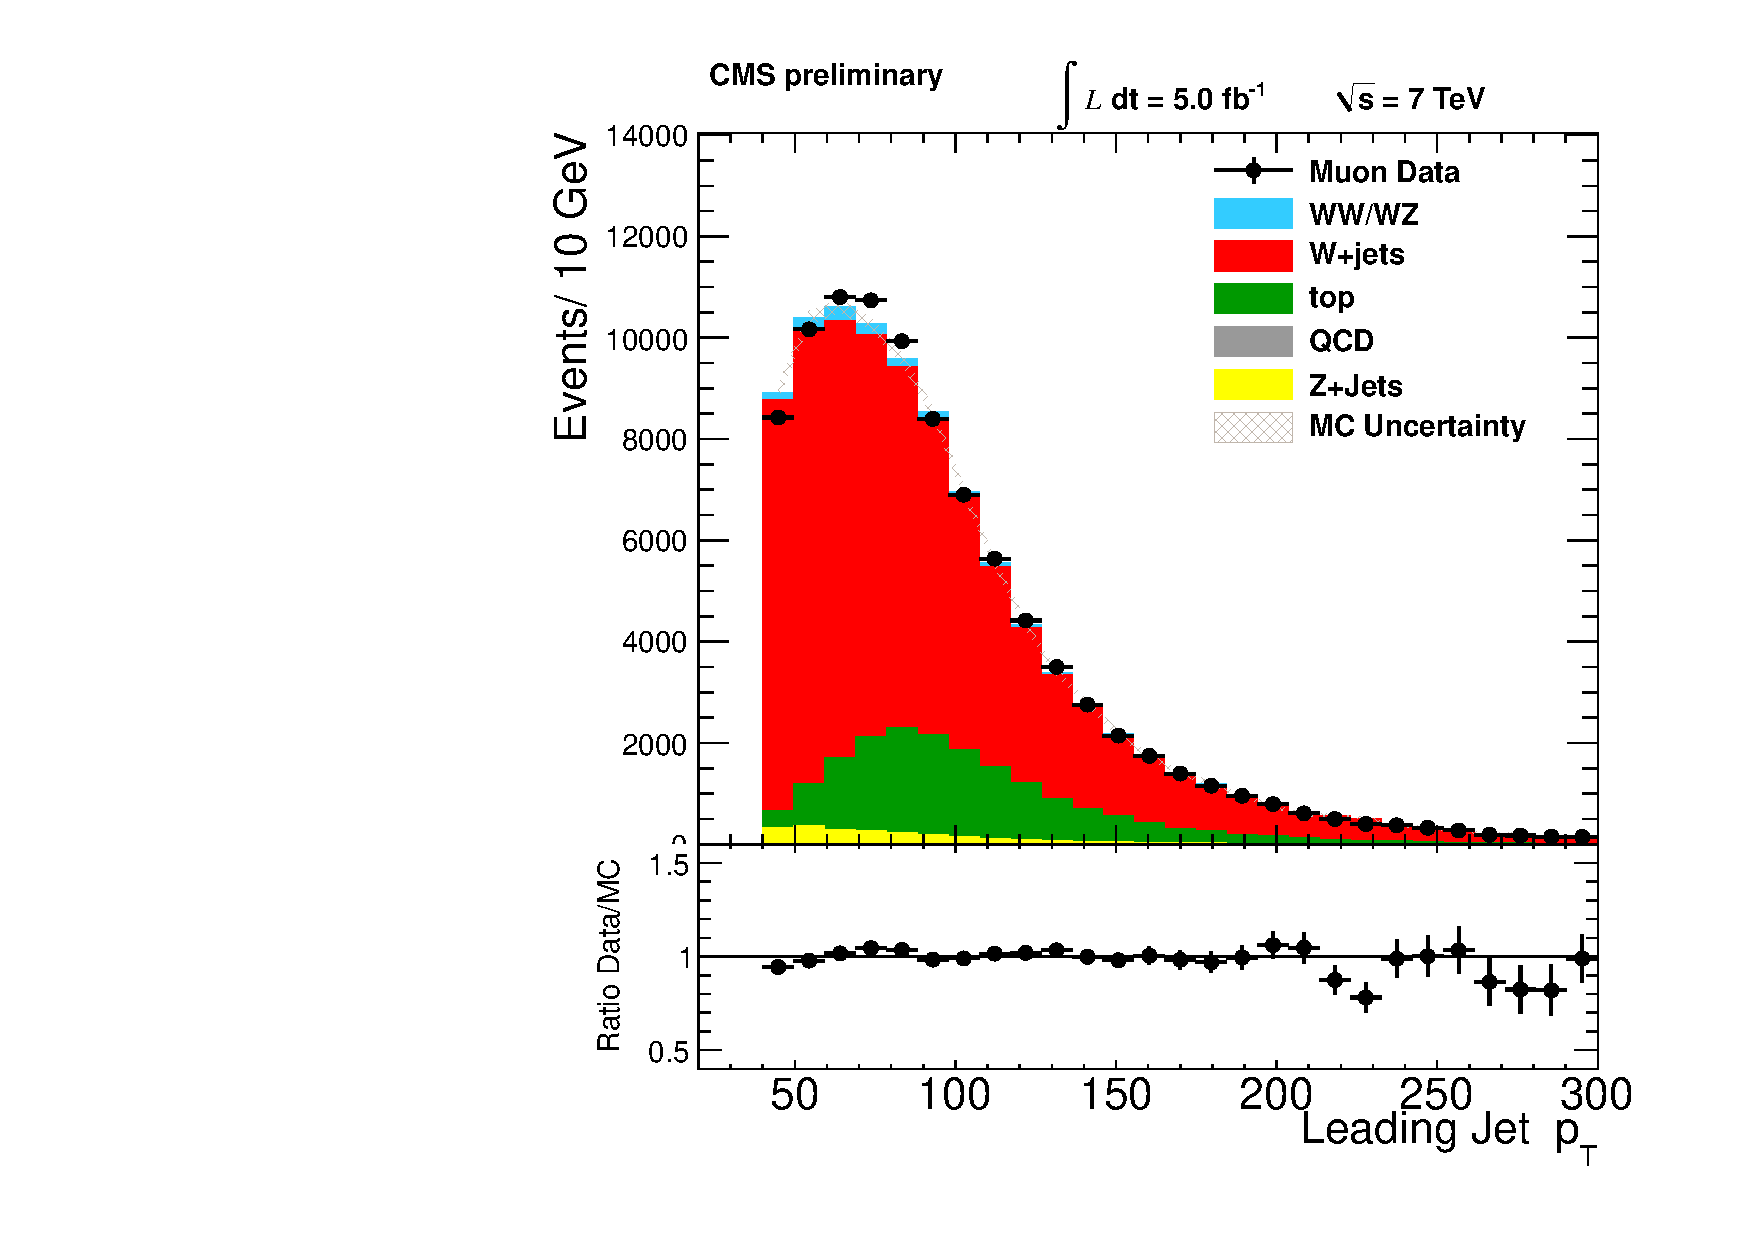
\includegraphics[width=0.49\textwidth]{figs/mu_jetld_pt.pdf}
    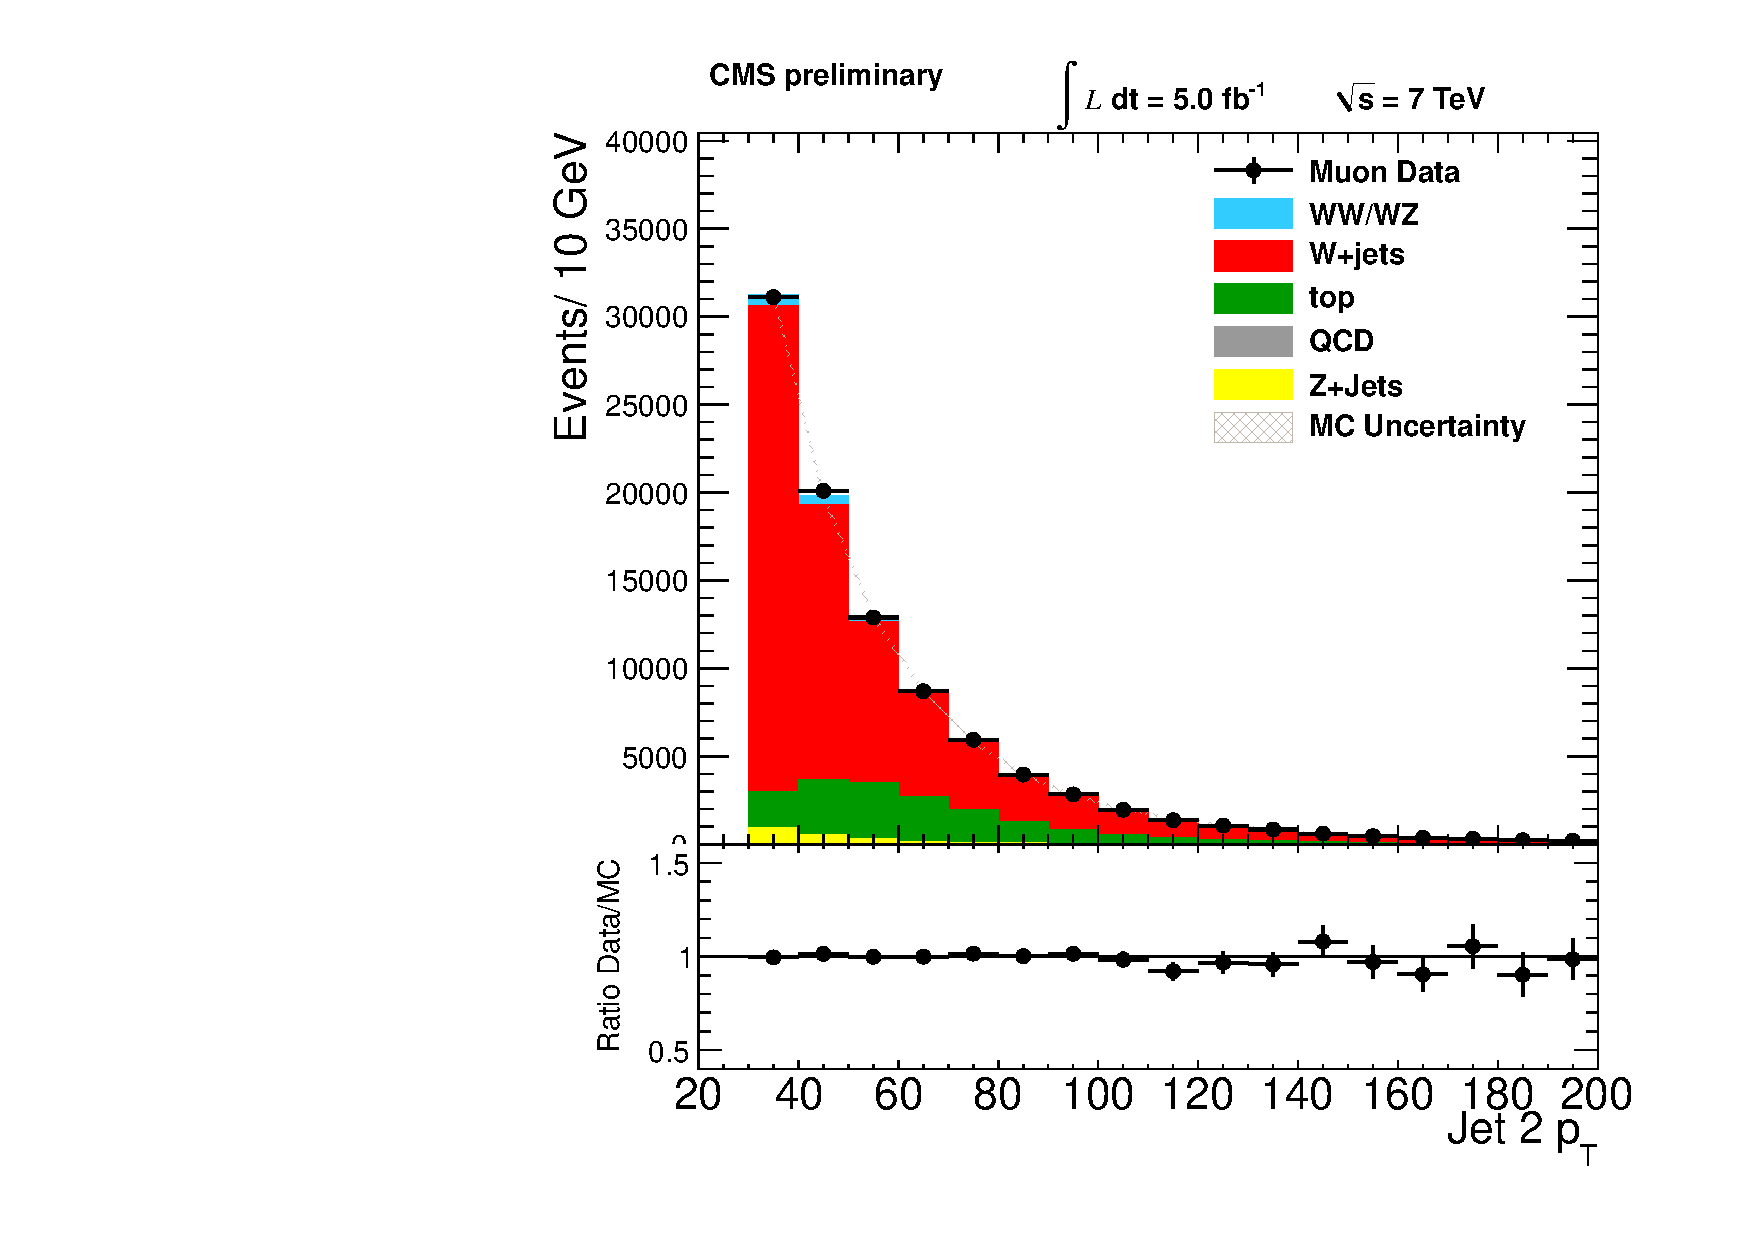
\includegraphics[width=0.49\textwidth]{figs/mu_jetnt_pt.pdf}
    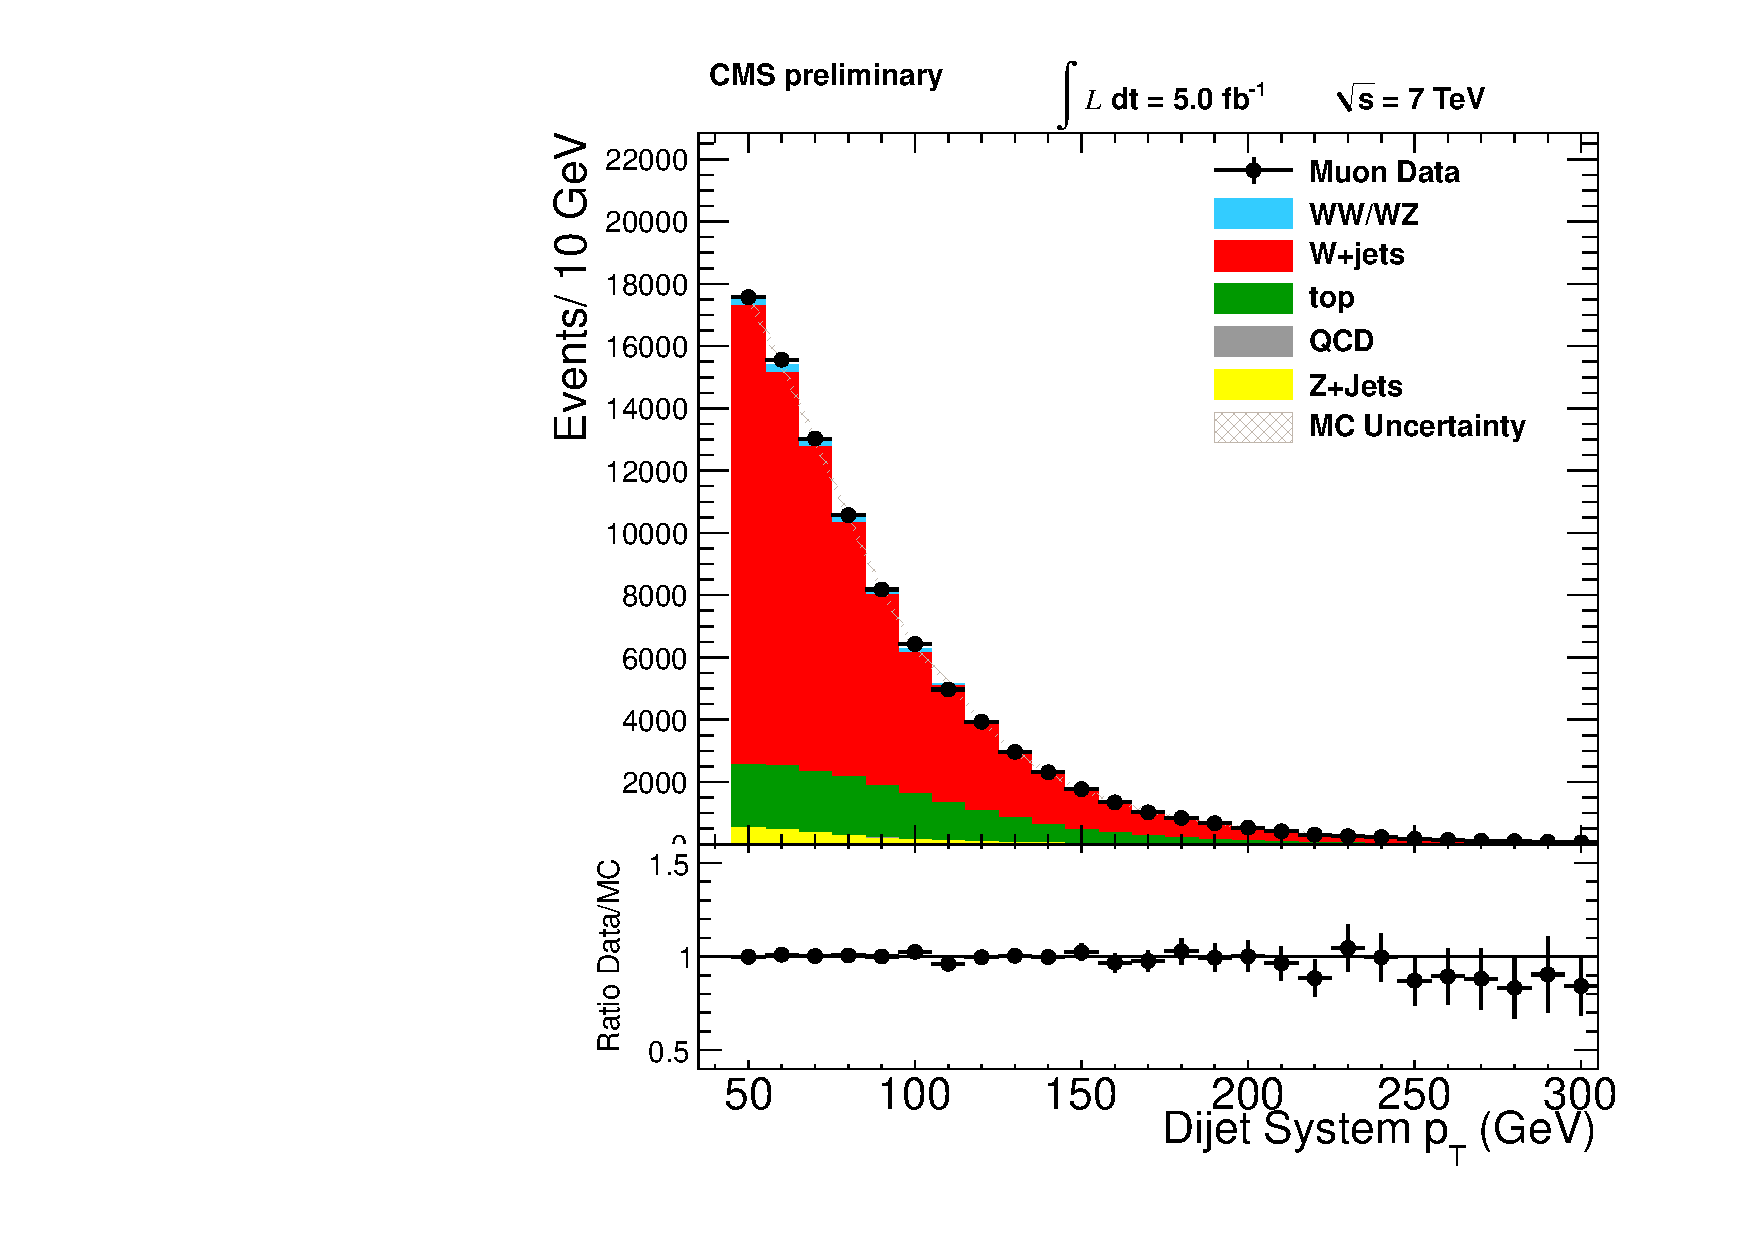
\includegraphics[width=0.49\textwidth]{figs/mu_dijet_pt.pdf}
    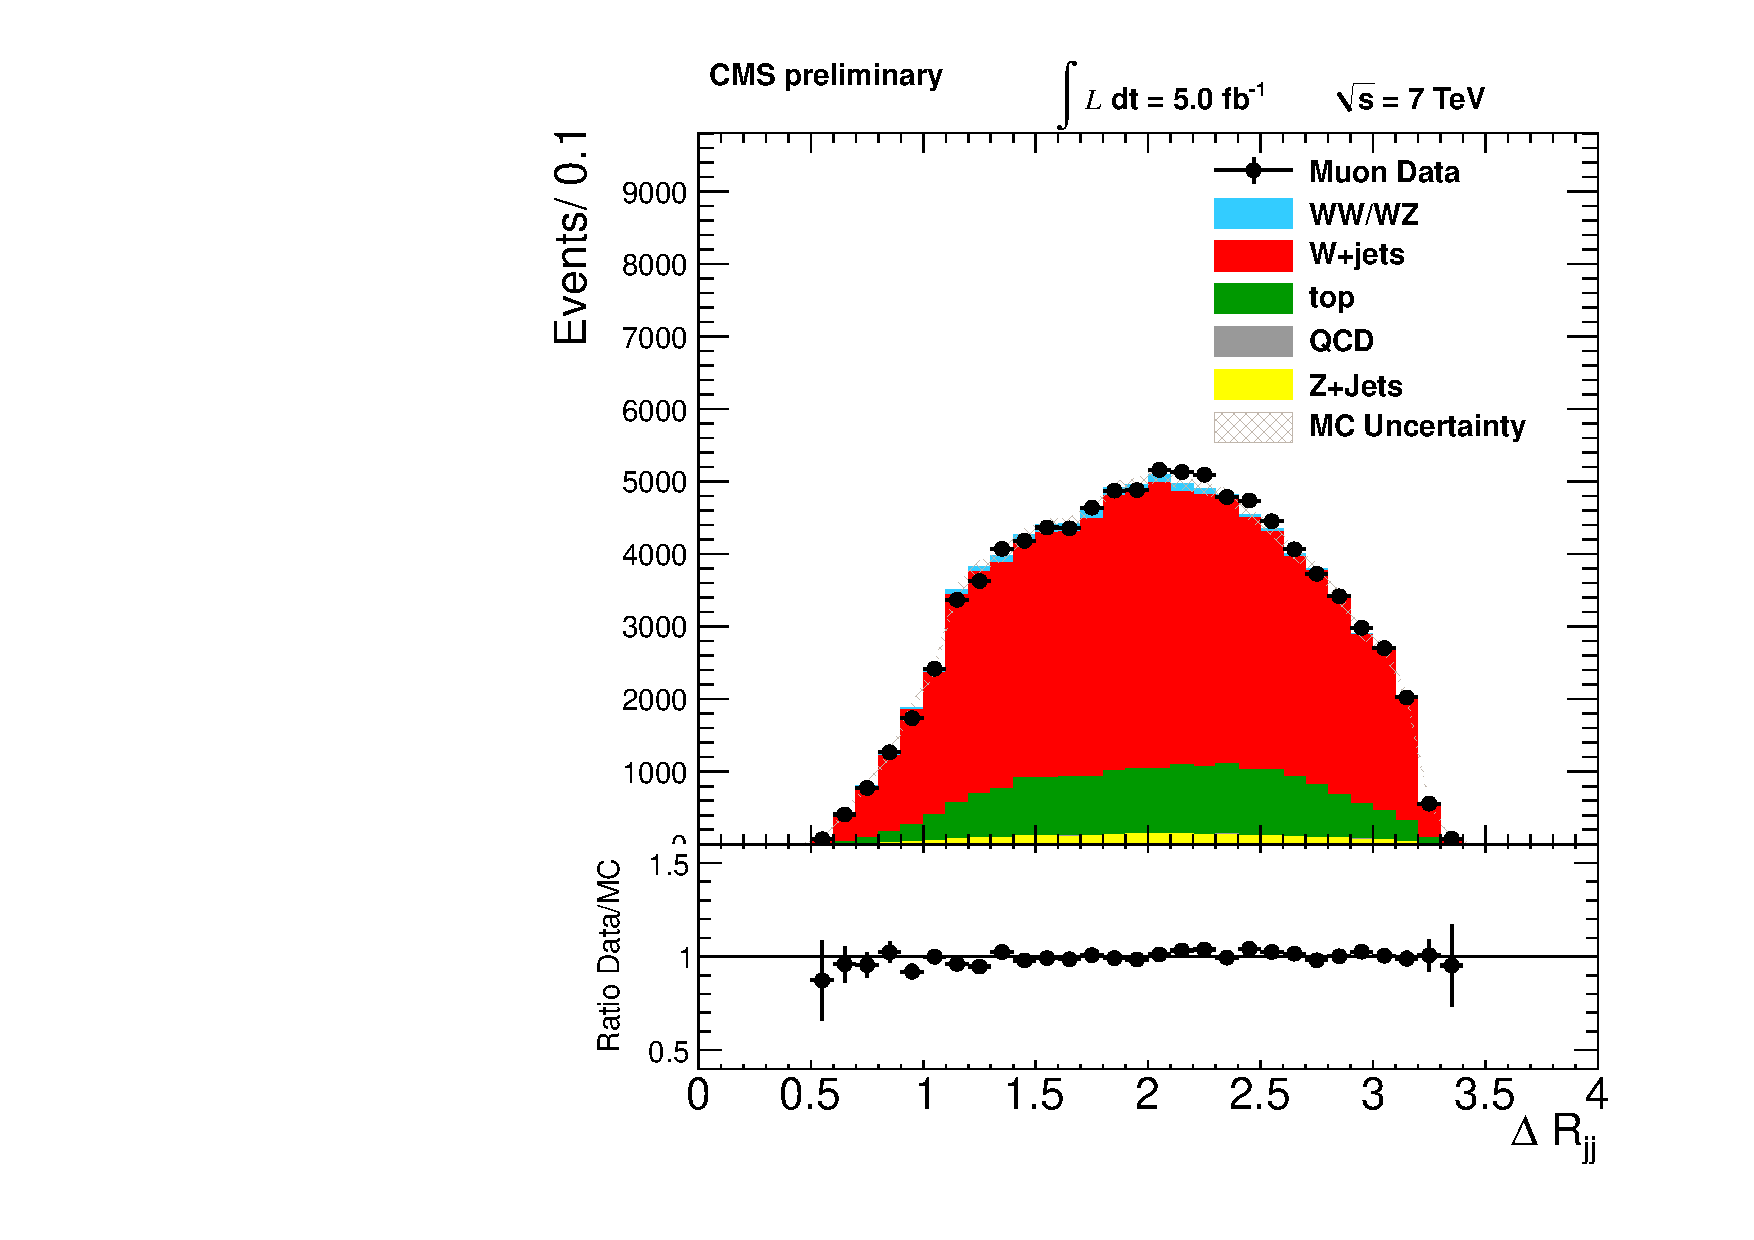
\includegraphics[width=0.49\textwidth]{figs/mu_deltaRjj.pdf}
    \caption{Comparison of the distributions in data and MC for the muon plus jets event sample after event selection 
    (upper left) of the transverse momentum of the leading jet, (upper right) of the transverse momentum of the 
    second leading jet, (lower left) of the dijet transverse momentum, (lower right) of the dijet distance parameter 
    $\Delta R= \sqrt{(\Delta \eta_{jj})^2 + (\Delta \phi_{jj})^2}$. The error bars on the data points are statistical only.
    The relative normalization of the various MC samples are taken from the result of the fit to the \mjj spectrum. 
%%The resulting
%%    MC histogram was normalized to the number of events in the data histogram.
    }}
\end{figure}

\begin{figure}[h!t]
  {\centering
    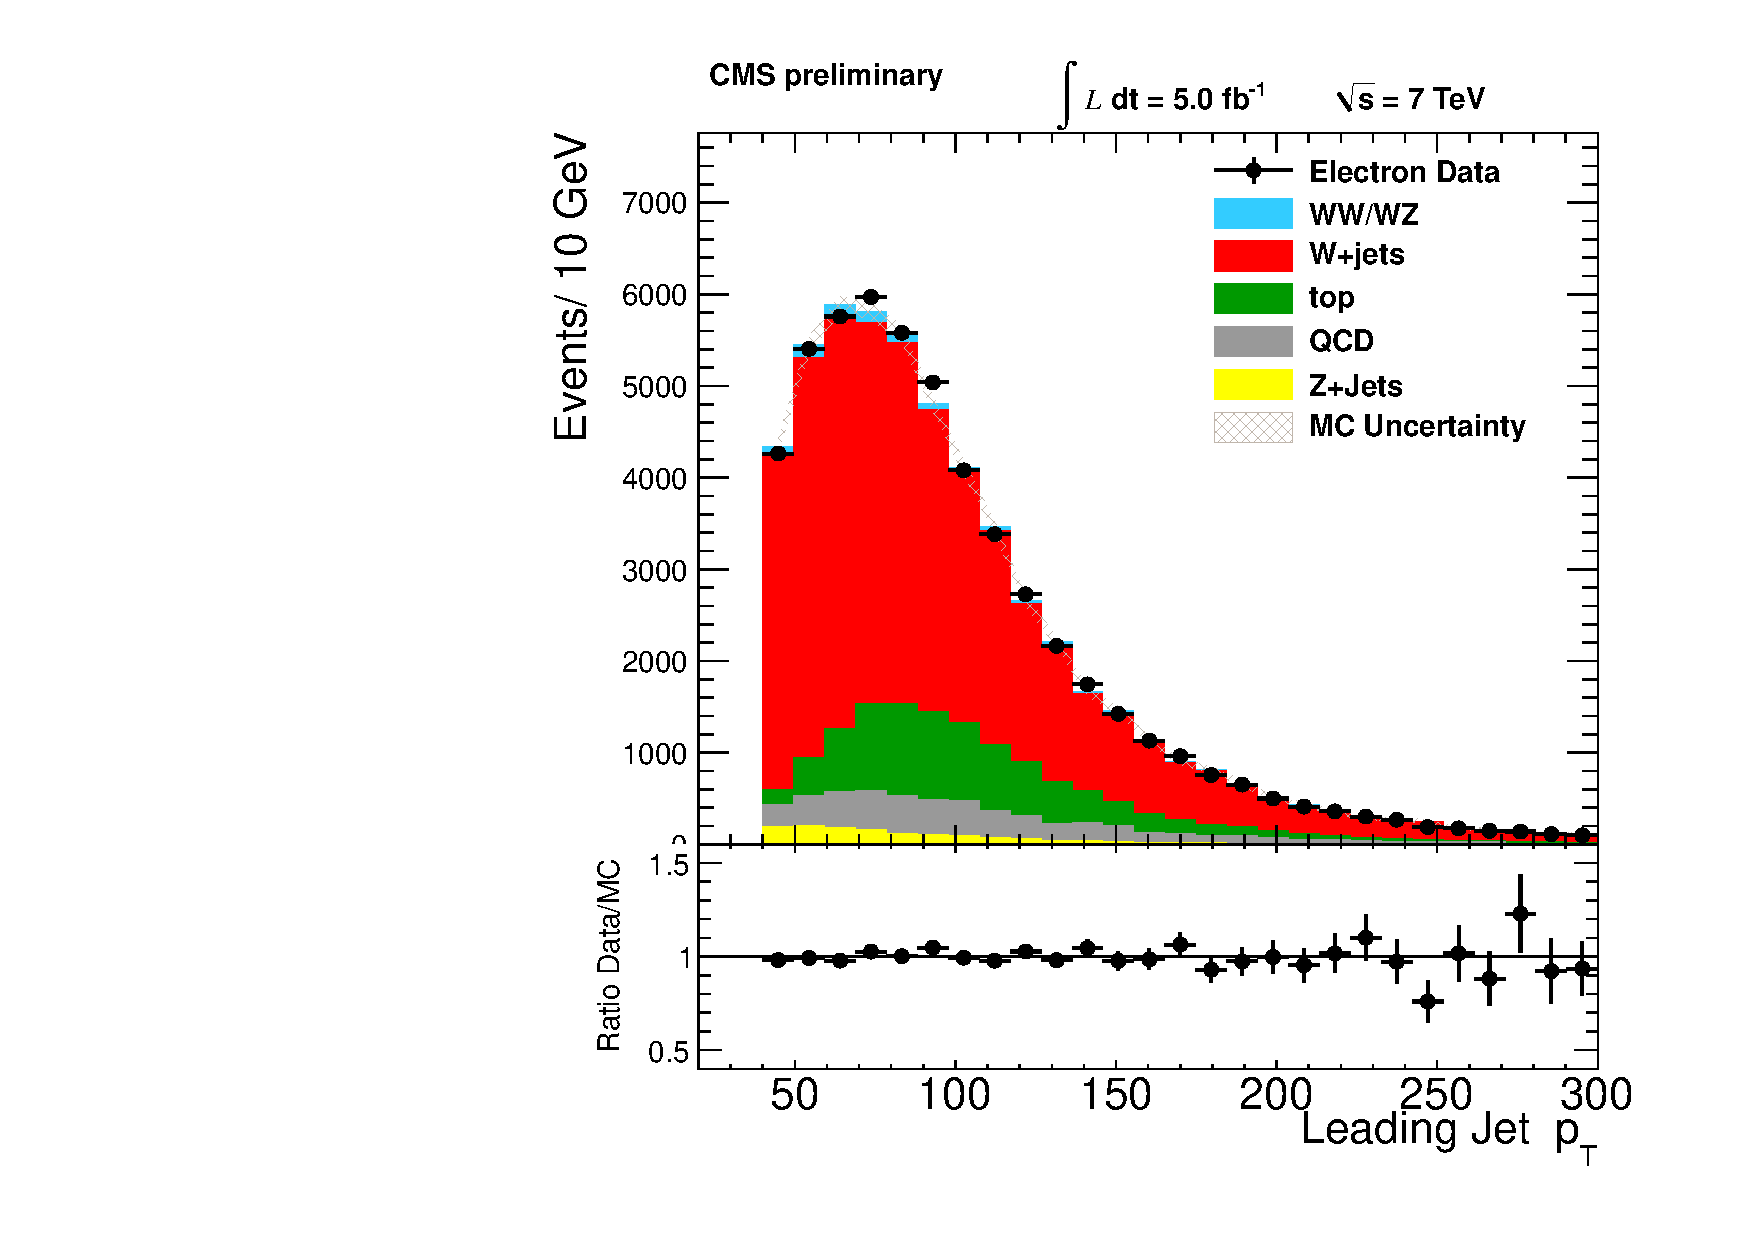
\includegraphics[width=0.49\textwidth]{figs/el_jetld_pt.pdf}
    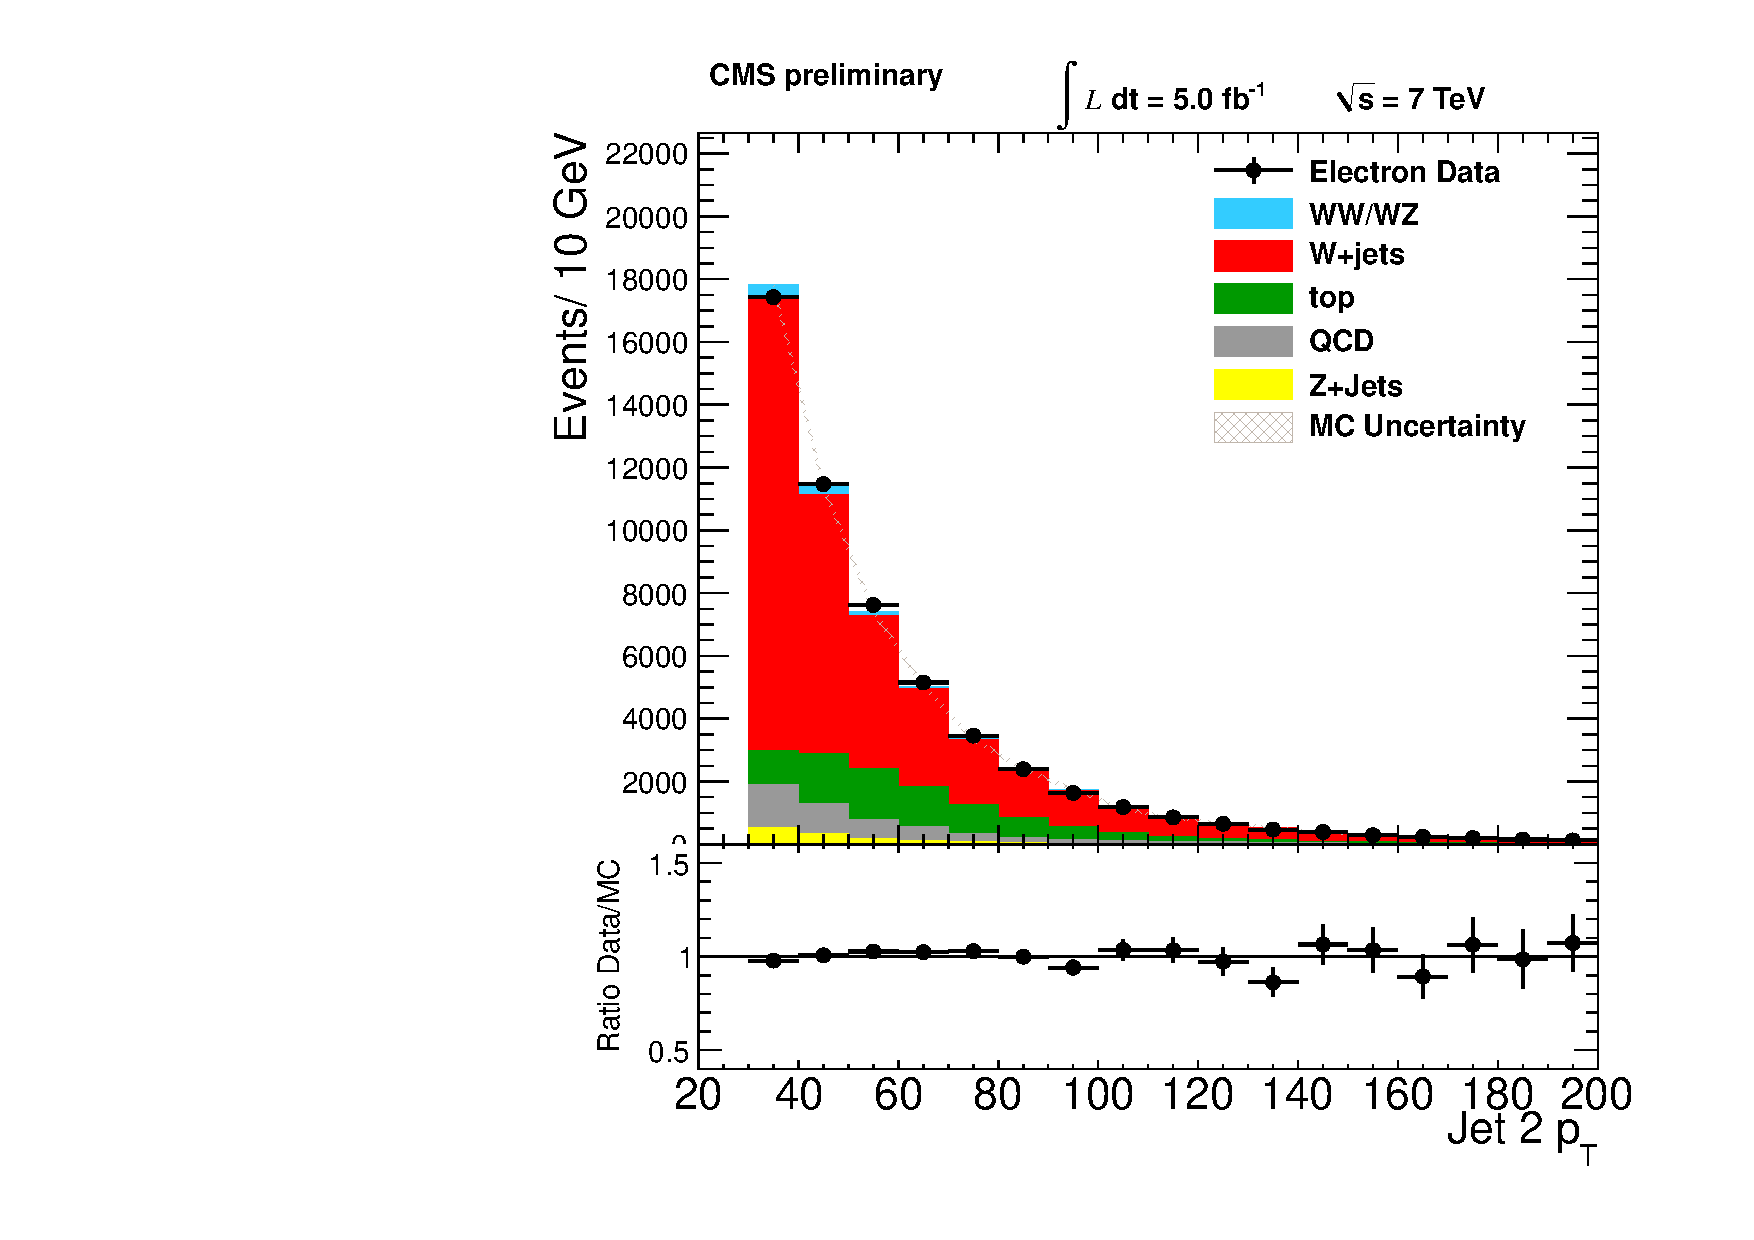
\includegraphics[width=0.49\textwidth]{figs/el_jetnt_pt.pdf}
    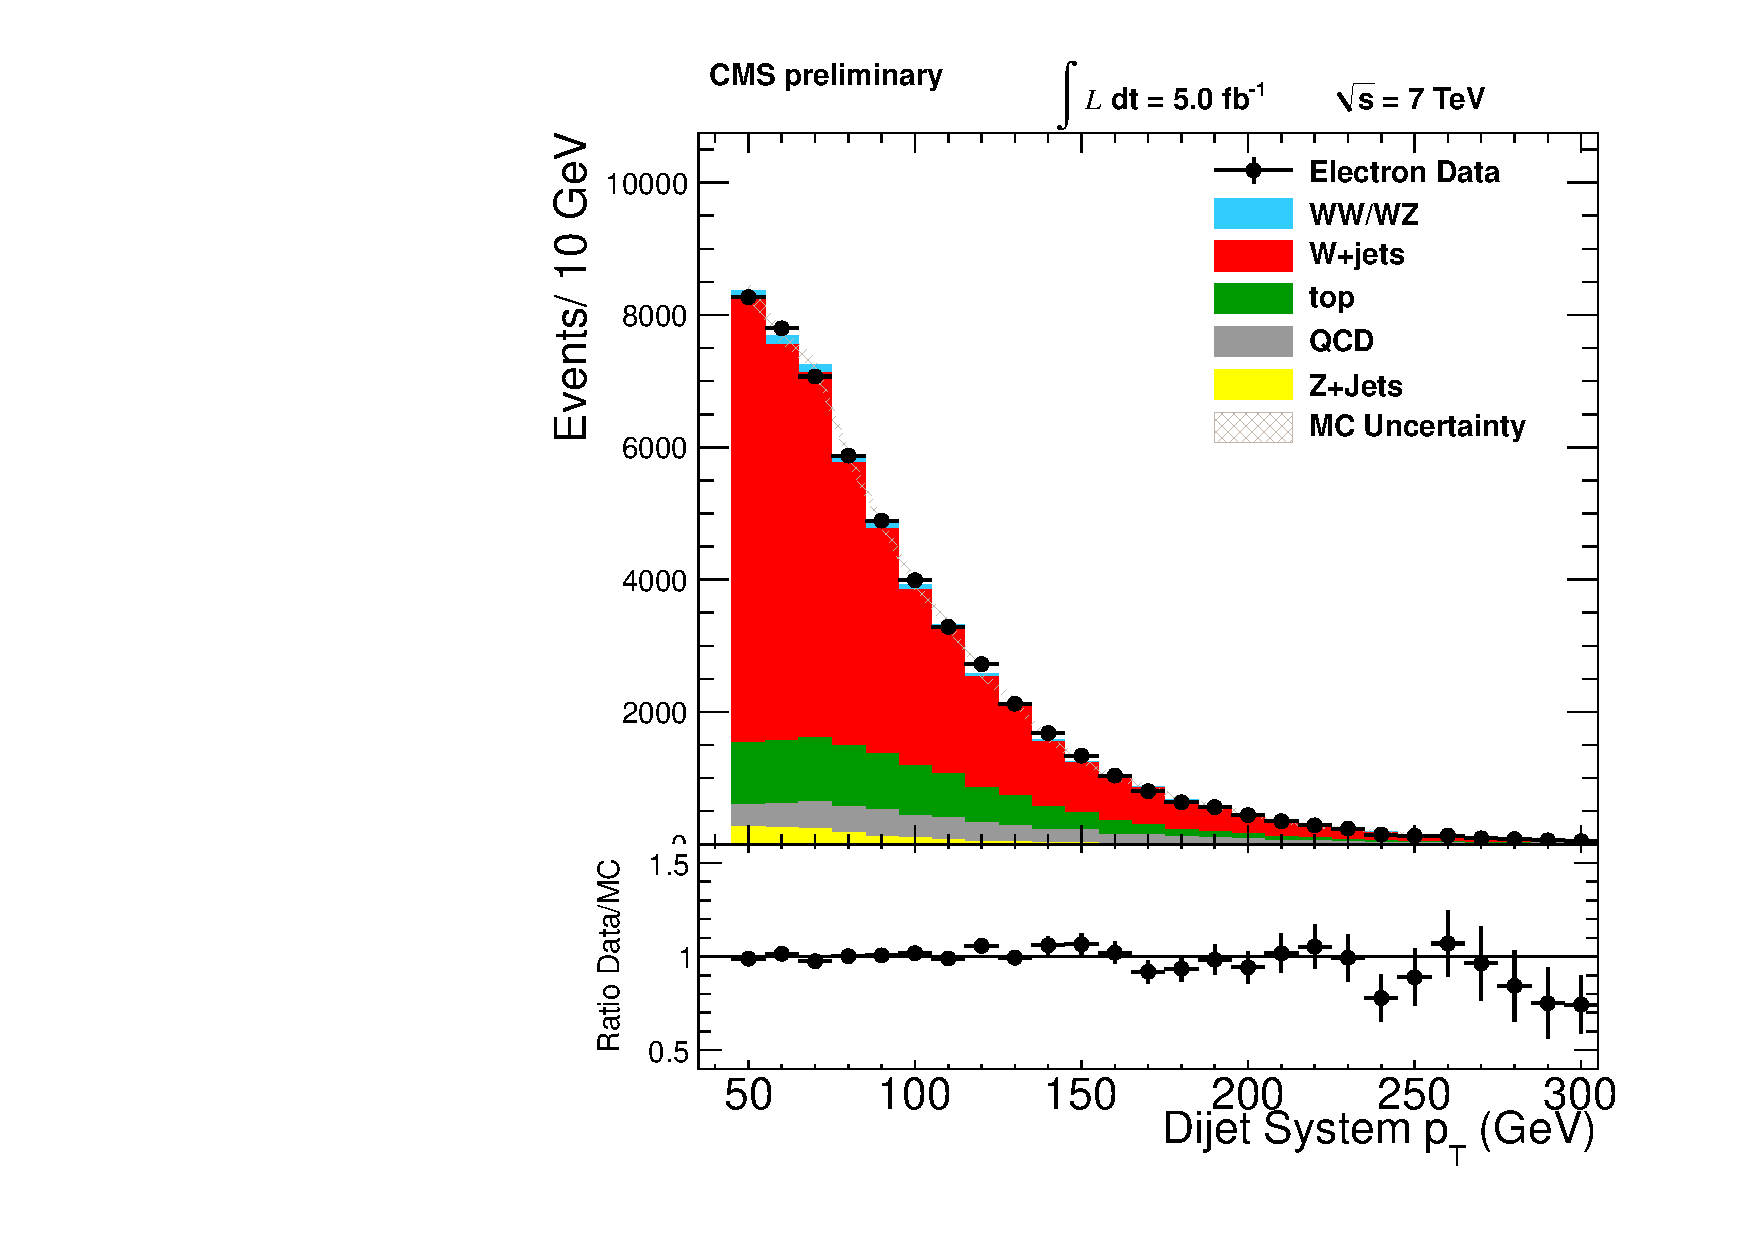
\includegraphics[width=0.49\textwidth]{figs/el_dijet_pt.pdf}
    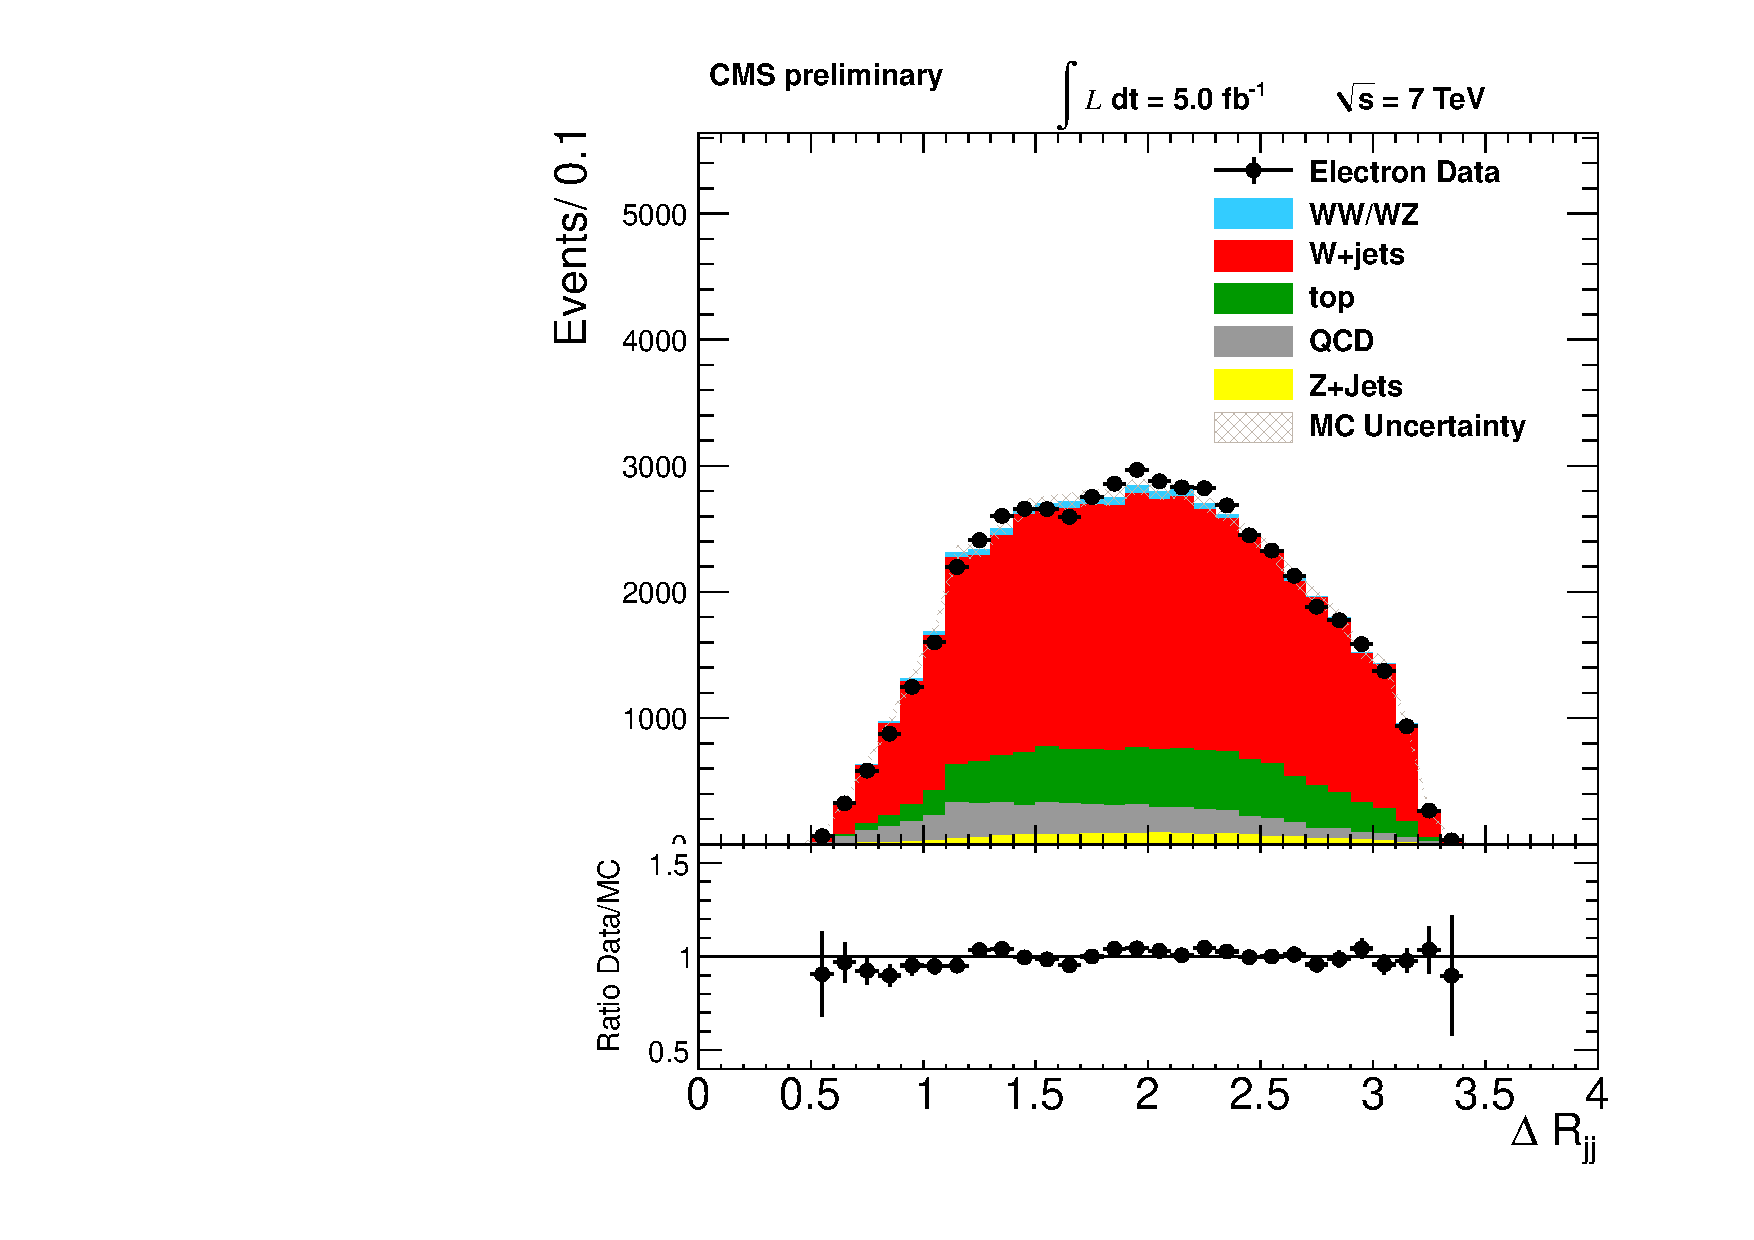
\includegraphics[width=0.49\textwidth]{figs/el_deltaRjj.pdf}
    \caption{Comparison of the distributions in data and MC for the electron plus jets event sample after event selection 
    (upper left) of the transverse momentum of the leading jet, (upper right) of the transverse momentum of the 
    second leading jet, (lower left) of the dijet transverse momentum, (lower right) of the dijet distance parameter 
    $\Delta R= \sqrt{(\Delta \eta_{jj})^2 + (\Delta \phi_{jj})^2}$. The error bars on the data points are statistical only.
    The relative normalization of the various MC samples are taken from the result of the fit to the \mjj spectrum. 
%%The resulting
%%    MC histogram was normalized to the number of events in the data histogram.
    }}
\end{figure}






%%% DO NOT ADD \end{document}!

















